\documentclass[11pt,a4paper]{article}
\usepackage[utf8]{inputenc}
\usepackage{graphicx}
\usepackage[table]{xcolor}
\usepackage[overlay,absolute]{textpos}
\usepackage[multiple]{footmisc}
\usepackage{fancyhdr}
\usepackage{hyperref}
\usepackage[top=35mm, bottom=35mm, left=35mm, right=30mm]{geometry}
\usepackage[style=ieee,autocite=inline,bibencoding=ascii,backend=bibtex]{biblatex}
\usepackage{xstring}
\usepackage{caption}
\usepackage{array}
\usepackage{float}
\usepackage{setspace}
\usepackage{pdflscape}
\usepackage[number]{abstract}
\usepackage{afterpage}
\usepackage{listings}
\usepackage{algpseudocode}
\usepackage{algorithm}
\usepackage{amsmath}
\usepackage{pgfgantt}
\usepackage{subcaption}
\usepackage{pdflscape}
\usepackage{cleveref}
\usepackage{pgf,tikz}
\usepackage{tikz}
\usepackage[utf8]{inputenc}
\usepackage[australian]{babel}
\usepackage[titletoc, header, title]{appendix}
\usepackage{physics}
\usepackage{pgfplots}

\pgfplotsset{compat=1.15}

\usepackage{minted}

\usetikzlibrary{patterns,decorations.pathmorphing,positioning}
\usetikzlibrary{arrows.meta,calc} %%% Add calc
\usetikzlibrary{external}
\tikzexternalize

\crefname{appsec}{Appendix}{Appendices}

%\singlespacing
\onehalfspacing
%\doublespacing

\fancyhf{} % clear all header and footers
\rfoot{\thepage}
\pagestyle{fancy}

% For inserting a blank page.
\newcommand{\blankpage}{
\clearpage
\thispagestyle{empty}
\mbox{}
\clearpage
\addtocounter{page}{-1}
}

\newcolumntype{L}[1]{>{\raggedright\let\newline\\\arraybackslash\hspace{0pt}}m{#1\textwidth}}
\newcolumntype{C}[1]{>{\centering\let\newline\\\arraybackslash\hspace{0pt}}m{#1\textwidth}}
\newcolumntype{R}[1]{>{\raggedleft\let\newline\\\arraybackslash\hspace{0pt}}m{#1\textwidth}}
\newcolumntype{P}[1]{>{\raggedright\right\newline\\\arraybackslash\hspace{0pt}}p{#1\textwidth}}

%% To prevent overfull hbox in bibliography.
\emergencystretch=1em

%%% Include bibtex references.
\addbibresource{references.bib}

\graphicspath{ {./figures/} }

\title{Final Report}
\author{Taylor Young\\Student Number: 3206230}

\begin{document}
%Title
\def\isfinalreport{1}
\begin{titlepage}
    \begin{center}
        % Upper part of the page. The '~' is needed because \\
        % only works if a paragraph has started.
        \begin{center}
            
\includegraphics[width=0.15\textwidth]{./figures/uon_logo.png}
            
            \textsc{\LARGE University of Newcastle}\\[1cm]
        \end{center}
        
        % Title
        % Author and supervisor
        \begin{textblock*}{133mm}(49mm,75mm)  %% change width of box from 10in as you wish
            \begin{minipage}[t][65mm][t]{133mm}
                \centering
                ~\\[0.5cm]
                \textsc{\Large Final Report}\\[0.5cm]
            
                \hrule ~\\[0.5cm]
                { \Large Pneumatic Muscle Joint Research and Design:\\ Software Framework and Muscle Design\\[0.5cm] }
                \hrule ~\\[0.5cm]
            
                \noindent
                \begin{minipage}{0.4\textwidth}
                    \begin{flushleft} \large
                        \emph{Author:}\\
                        Taylor \textsc{Young}\\
                        Student Number: 3206230
                    \end{flushleft}
                \end{minipage}%
                \begin{minipage}{0.4\textwidth}
                    \begin{flushright} \large
                        \emph{Supervisor:} \\
                        Colin \textsc{Coates}\\
                    \end{flushright}
                \end{minipage}\\[0.5cm]
                \hrule ~\\[0.3cm]
                {\large \today}
            \end{minipage}
        \end{textblock*}
    \end{center}
    
    \vfill
    
    \emph{A thesis submitted in partial fulfilment of the requirements for the degree of Bachelor of Engineering in Electrical Engineering at The University of Newcastle, Australia.}
    
    \vfill
\end{titlepage}

% pdflatex -synctex=1 -shell-escape Final_Report.tex
\blankpage
\pagenumbering{gobble}

%%% Use roman numerals for page numbering in document preamble (abstract, TOC, acknowledgements, etc).
\pagenumbering{roman}

%Abstract
\section*{Abstract}
\addcontentsline{toc}{section}{Abstract}
Humanoid robotics is a fast-developing field encompassing a wide range of engineering disciplines to solve the challenges of robotic interaction in environments designed for humans. In order to encourage this development many competitions exist around very common but highly specific human tasks. These all aim to extend the field of humanoid robotics and general intelligence.
In order to be a humanoid robot, a key feature is the ability to walk, robots need some method of actuating joints in a controllable, fast and energy efficient way.\newline
This project is to design and construct a single leg, based on a custom developed humanoid robotic platform. Specifically focusing on the knee and ankle joints. A single degree of freedom test rig has been constructed to test the feasibility of both the pneumatic muscles and the control scheme.
A mathematical model for the actuator has been used to inform the control system structure and allow the estimation of the current system state. Pneumatic muscles are a highly nonlinear actuator, this means that standard linear controllers have limited success in controlling the actuator position. Control can be achieved with only a static force map leading to an accurate, high-performance control scheme, however, pneumatic muscles also have their own dynamics, like hysteresis, some thermodynamic effects. \newline
Therefore, a nonlinear MPC controller has been implemented and theoretically compared to two other standard controllers. \newline
\blankpage

%Acknowledgements
\section*{Acknowledgements}
\addcontentsline{toc}{section}{Acknowledgements}
\raggedright\hfill\break

TODO
\blankpage

%Contributions
\section*{Contributions}
\addcontentsline{toc}{section}{Contributions}

The project described in this thesis is based in the discipline of Electrical Engineering. The key contributions to this project are listed below:

\begin{itemize}
    \item Performed a literature review of:
    \begin{itemize}
        \item Pneumatic Air Muscle design parameters and construction,
        \item Various non-linear control methods,
        \item Static and Dynamic system modelling,
    \end{itemize}
    \item Designed a adult sized pneumatic leg based on pneumatic muscles,
    \item Designed and constructed a single degree of freedom pneumatic muscle test rig,
    \item Researched and constructed various pneumatic muscles to determine material compatibility,
    \item Designed a modular software framework that allows the use of varying controllers and system arrangements,
    \item Implemented a SMC controller,
    \item Designed and and implemented a MPC based controller and optimiser. 
    \item Implemeted a simulated pneumatic muscle plant.
\end{itemize}

\raggedright\hfill\break\vfill

\noindent\begin{tabular}{ll}
    \makebox[2.5in]{\hrulefill} & \makebox[2.5in]{\hrulefill}\\
    Taylor Young & Date\\[8ex]% adds space between the two sets of signatures
    
    \makebox[2.5in]{\hrulefill} & \makebox[2.5in]{\hrulefill}\\
    Colin Coates & Date\\
\end{tabular}


\blankpage

%Contents
\tableofcontents
\clearpage

%%% Use arabic numbers for page numbering in report body.
\pagenumbering{arabic}

\section{Introduction}
\label{sec:introduction}

\subsection{Motivation}
\label{sub:motivation}


Humanoid robotics is a fast-developing field encompassing a wide range of engineering disciplines to solve the challenges of robotics interaction in an environment designed for humans. In order to encourage this development many competitions exist around very common but highly specific human tasks, all of which aim to extend the field of humanoid robotics and general artificial intelligence. Robocup \cite{kitano1995robocup}, is just one example of a competition utilising a simple concept, a soccer game, as the platform for the research and development of humanoid robots. Robocup involves teams of humanoid robots attempting to play a game of soccer on a scaled soccer field. Whilst this may seem trivial, in order to play soccer, you need the ability to perform three major tasks. These three tasks consist of vision, localisation, and locomotion. Vision is used to locate objects in the world, balls, goals, field lines and obstacles. This system provides the majority of the information input into the system which is then used to determine the various behaviours and actions to take. Localisation is responsible for determining whether the information is correct and consistent with the previous input data, filtering this information into what the robot perceives as the current world state. The last major system, locomotion, then allows the robot to move about the world to some desired location determined by the behaviour system. In order to perform this task, the robot needs some method of actuating joints in a controllable, fast and energy efficient way. Currently, actuators used by different humanoid league teams are limited to two main products, dynamixel servos \cite{robotis_mx106} or custom designed servo motors. These are both expensive and are limited in the speed and torque which can be output from the actuator. Both of these methods use electrical energy as the main energy system, storing this within Li-Po batteries and converting to a rotating shaft via a motor and gearbox. However, major leaders in the field of humanoid robotics and robotics in general outside of this competition use hydraulics \cite{atlas}. This allows them to carry larger payloads and run for longer periods of time. However, this also has it's trade offs increasing the weight of the platform and the speed in which it can move. \newline

Thus the ultimate motivation for this project is to design and construct an alternate actuator capable of out performing the currently used dynamixel actuators in the performance of speed, energy efficiency and torque. \newline

This specific stage of the project will focus on the development of a software framework to ease the design of new controllers for pneumatic muscles. A test rig will also be developed that replicates the motion of the single degree of freedom knee joint proposed in the leg design.

\subsection{Overview}
\label{sub:overview}

As a whole this project is to design and construct a single leg based on a custom developed humanoid robotic platform, focusing on the knee and ankle joints specifically. A mathematical model for the actuator will be used to inform the control system structure and allow the estimation of the current system state. The performance criteria for the actuator will be compared against two currently used dynamixel servos, the MX-106 \cite{robotis_mx106} and XM-540 \cite{robotis}.

Specifically the work to be undertaken within this stage of the project comprises of the design and construction of a single degree of freedom joint which can be position controlled. The work will focus of developing a robust non-linear controller capable of driving a pair of pneumatic muscles via commands sent from a microcontroller. Various sensors will be used to determine the current state of the pneumatic muscles, of which will interface to the microcontroller via a custom PCB shield. The work will focus on developing a framework for the future expansion of the controller to move advanced control schemes, laying a suitable software platform for increased degrees of freedom and muscles.

\clearpage
\subsection{Outline}
\label{sub:outline}

This report has been organised into five major sections, related work, system implementation and electronics, modelling and control, software architecture, and simulated system.

\begin{enumerate}
\item \textbf{Related Work} The current research relevant to the specified project is broken into three major areas. The design and construction of functioning pneumatic muscles, control methods used to control linear and non linear systems, and methods of modelling static and dynamic systems.

\item \textbf{System Implementation and Electronics}
The system implementation covers a leg platform design, as well as a 1 DoF test rig design and construction. Muscle design and Pneumatic control are covered following the electronics used within the test rig system.

\item \textbf{Modelling and Control}
This section covers modelling and control of the pneumatic muscles, with experimental results of the static modelling. It contains a detailed overview of the control structure.

\item \textbf{Software Architecture}
An overview of the software architecture with a breakdown of the modularity of the code base is covered in this section. The control structure performance is also analysed.

\item \textbf{Simulated System}
This section covers the implementation of a simulated plant to access controller performance.

\item \textbf{Conclusion} 
Finally, the conclusion will summarise the findings of this work. It contains recommendations for future works.

\end{enumerate}

\clearpage
\section{Related Work}
\label{sec:related_work}

The follow chapter outlines the current research relevant to the specified project. This project can be defined into three major areas, the design and construction of functioning pneumatic muscles, control methods used to control linear and non linear systems, and methods of modelling static and dynamic systems. 

\subsection{Pneumatic Muscles}
\label{sub:pneumatic_muscles}
Pneumatic air muscles have many names fluidic muscle, pneumatic muscle actuator, air muscle, axially contractible actuator, tension actuator, fluid actuator and fluid driven tension actuator \cite{najmuddin_mustaffa_2017} \cite{lau_chai_2012}. These are often shortened to PAM (pneumatic air muscle) or PMA (pneumatic muscle actuator) and are used interchangeably throughout research. PAM were first developed under the name McKibben Artificial Muscle in the 1950s for use in prosthetic limbs, they were then commercialised by the Bridgestone rubber company in the 1980s under the name Rubbertuators. Since then two major companies have developed PAMs for commercial purposes, Festo and the Shadow Robot Company. \Cref{fig:pneumatic_design} shows the construction of pneumatic muscles consisting of an outer braided mesh and inner rubber or latex bladder. At one end the bladder has an air tight seal with the braided mesh fixed in place. At the other end it contains an inlet for the compressed air. PAM typically require external sensing mechanisms due to their nonlinear behaviours; these often measure pressure, axial contraction and exerted force of the actuator \cite{erin_pol_valle_park_2016}. \newline

Pneumatic muscles are analogous to the "biological motor" for locomotion or manipulation with advantages like the passive damping, good power to weight ratio, low maintenance, low price and usage in rough environments \cite{ranjan_upadhyay_kumar_dhyani_2012}. They are ideal for use in human environments in applications of human interaction such as rehabilitation therapy, nursing elderly people, and day to day work support for elderly people \cite{saga_nagase_saikawa_2006}. Compared to traditional actuators in the form of electric servos, pneumatic muscles are highly nonlinear requiring complex controllers to perform precise movements. \newline

% TODO Make this picture a picture of mine with better labels
\begin{figure}[ht!]
    \centering
    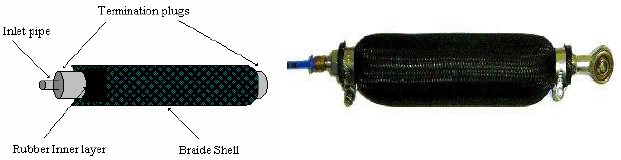
\includegraphics[scale=0.6]{Pneumatic-Muscle-Actuator-Design.png}
    \caption{Pneumatic Muscle Actuator Design \cite{pneumatic_image}}
    \label{fig:pneumatic_design}
\end{figure}

Previous studies have looked at alternate sensing methods utilising self-contained displacement and force sensors removing the requirement for external sensing elements that allow the detection of axial contraction force and displacement at the same time. Traditionally, linear encoders and load cells have been used to fulfil this task increasing the devices pysical size and form factor whilst also reducing the compliance, both of which are ascpects seen in human muscles. Existing solutions include dielectric elastomers, embedded microfluidic elastomers, conductive fibre mesh and inductive coils all of which use changing resistance or inductance to measure the displacement. These mechanisms often require special manufacturing processes that limit the selection of the elastomer \cite{erin_pol_valle_park_2016}. 
Additionally, research has focused on the compatibility between the braided mesh and the inner bladder. The suitability of the mesh is significant, using the optimum size braided mesh can lead to maximum contraction. 

Typically, PAM technology provides a maximum contraction of 25-30\% stroke compared to the 50-70\% stroke of the biological muscle \cite{andrikopoulos_nikolakopoulos_2017}. However, when the component dimensions are optimised contraction up to 51.85\% can be achieved \cite{najmuddin_mustaffa_2017}. Incompatibility of the braided mesh with the bladder forms stress regions where the bladder non-uniformly expands. When this happens, the energy is lost, and the contraction percentage is reduced. \newline

The force generated by the pneumatic muscle is dependent on the air pressure, nominal length, contraction ratio and material properties. When the air pressure rises, the muscle circumference increases while its length decreases, causing an increase in the muscle contraction. The resulting pulling force, acting in the axial direction, corresponds to the stresses in the flexible mesh. By controlling pressure, it is possible to control the pulling force and the contraction ratio of the pneumatic muscle. \newline

In order to control the flow of air in and out of the actuator an electrically controlled pneumatic proportional/servo valve can be used to adjust the flow of air. Whilst a proportional valve provides the best continuous flow behaviour, these are expensive, and to control a single muscle would require one on the input and one on the output. As an alternatve the use of on/off solenoid 3-way 3 port valves can be used, these often are controlled via a pulse width modulation (PWM) signal to approximate proportional valves. However, this frequent valve switching can lead to shorter valve life, reducing the viability of these valves \cite{zhang_bone_2018}. In order to reduce excessive valve switching a sliding-mode control (SMC) algorithm with three operating modes can be implemented ensuring the valves switch only when it is necessary for the desired closed-loop performance. This will be discussed in further detail in the control section of this paper \Cref{sub:sliding_mode_control}. \newline

Numerous studies have been presented into the feasibility of various robotic platforms based around the use of pneumatic muscles. Humanoid Robotic Leg (HURL) was a conceptual 10 degree of freedom (DOF) lower-limb humanoid platform that was a bio-metrically informed mechanical design that attempted to improve biped robots \cite{andrikopoulos_nikolakopoulos_2017}. This research only implemented the ankle joint concluding that a more complex control structure for torque and compliance control was required, utilising a dynamic model for increased performance. Similarly, a quadruped robot driven by Festo air muscles was designed to be a test bed for the implementation and control of pneumatic muscles in legged locomotion. This work suggests the inclusion of a model for the Festo air muscle that incorporates the kinematics of the platform should be implemented in future works \cite{aschenbeck_kern_bachmann_quinn}. Anthropomorphic robotic hand designs have also been designed with the goal of achieving basic human hand grasps. These use nylon tendon-like cables to transmit the power from a forearm section containing the muscles to the end effectors making them suitable for delicate object manipulation \cite{lau_chai_2012}.

\subsection{Control Methods}
\label{sub:control_methods}
As mentioned in \Cref{sub:pneumatic_muscles}, pneumatic muscles are a highly nonlinear actuator. This means that standard linear controllers have limited success in controlling the actuator position. Often it is possible to linearise a nonlinear plant around some known operating region in order to implement linear control structures. This could be utilised to control pneumatic muscles if the response curve of the actuator had a useful near linear region to linearise about. However, as seen later in \Cref{sub:system_modelling} this is not the case and thus a controller designed to handle nonlinear properties should be used. 

\subsubsection{ANPID - Advanced Non-linear Proportional Integral Differential}
\label{sub:pid}
Advanced nonlinear proportional integral differential (ANPID) controllers are an extension of a linear control structure (PID) that attempts to provide an advanced, flexible and adjustable control performance for custom applications, without requiring knowledge of the setups model. These can be difficult to fine tune the control parameters to achieve efficient control performance and can require an additional layer to schedule gains of the system according to the operating regions and movement type \cite{andrikopoulos_nikolakopoulos_2017}. This scheme lends itself to applications where the system dynamics are unknown and difficult to measure. Generally, this isn't a restriction faced when developing a platform from the ground up and thus implementing a control structure that has an increased knowledge of the system dynamics should be used.

\subsubsection{Model Predictive Control}
\label{sub:model_predictive_control}
Model predictive control is a method for dealing with multi-variable control problems. It aims to choose a control state by solving the system state model repeatedly, with the goal of minimising the error function into the future horizon. The behaviour is based on a plant model and is highly dependant on the accuracy of this model. Model predictive control is a broader term used to cover a variety of linear and nonlinear control structures including Kalman and Unscented Kalman Filters.\newline
A structure of MPC typically used in the control of highly non-linear systems utilise an optimiser. The job of the optimiser is to calculate the cost of performing a series of input variations in terms of the system error. The optimiser is run p times over the prediction horizon, forming a prediction of the output based on some predicted control input. This is performed for many differing first control inputs. The error between the reference trajectory and predicted output is than ranked to find the lowest cost. The first predicted control input of the lowest cost itteration is then used and the time updated. Typically a sample time that allows 10 to 20 samples over the rise time of the system is used. The prediction horizon should cover 20 to 30 samples over the transient response of the system. The prediction horizon show then be 10 to 20\% of the prediction horizon.\newline

\begin{figure}[!hbt]
    \centering
    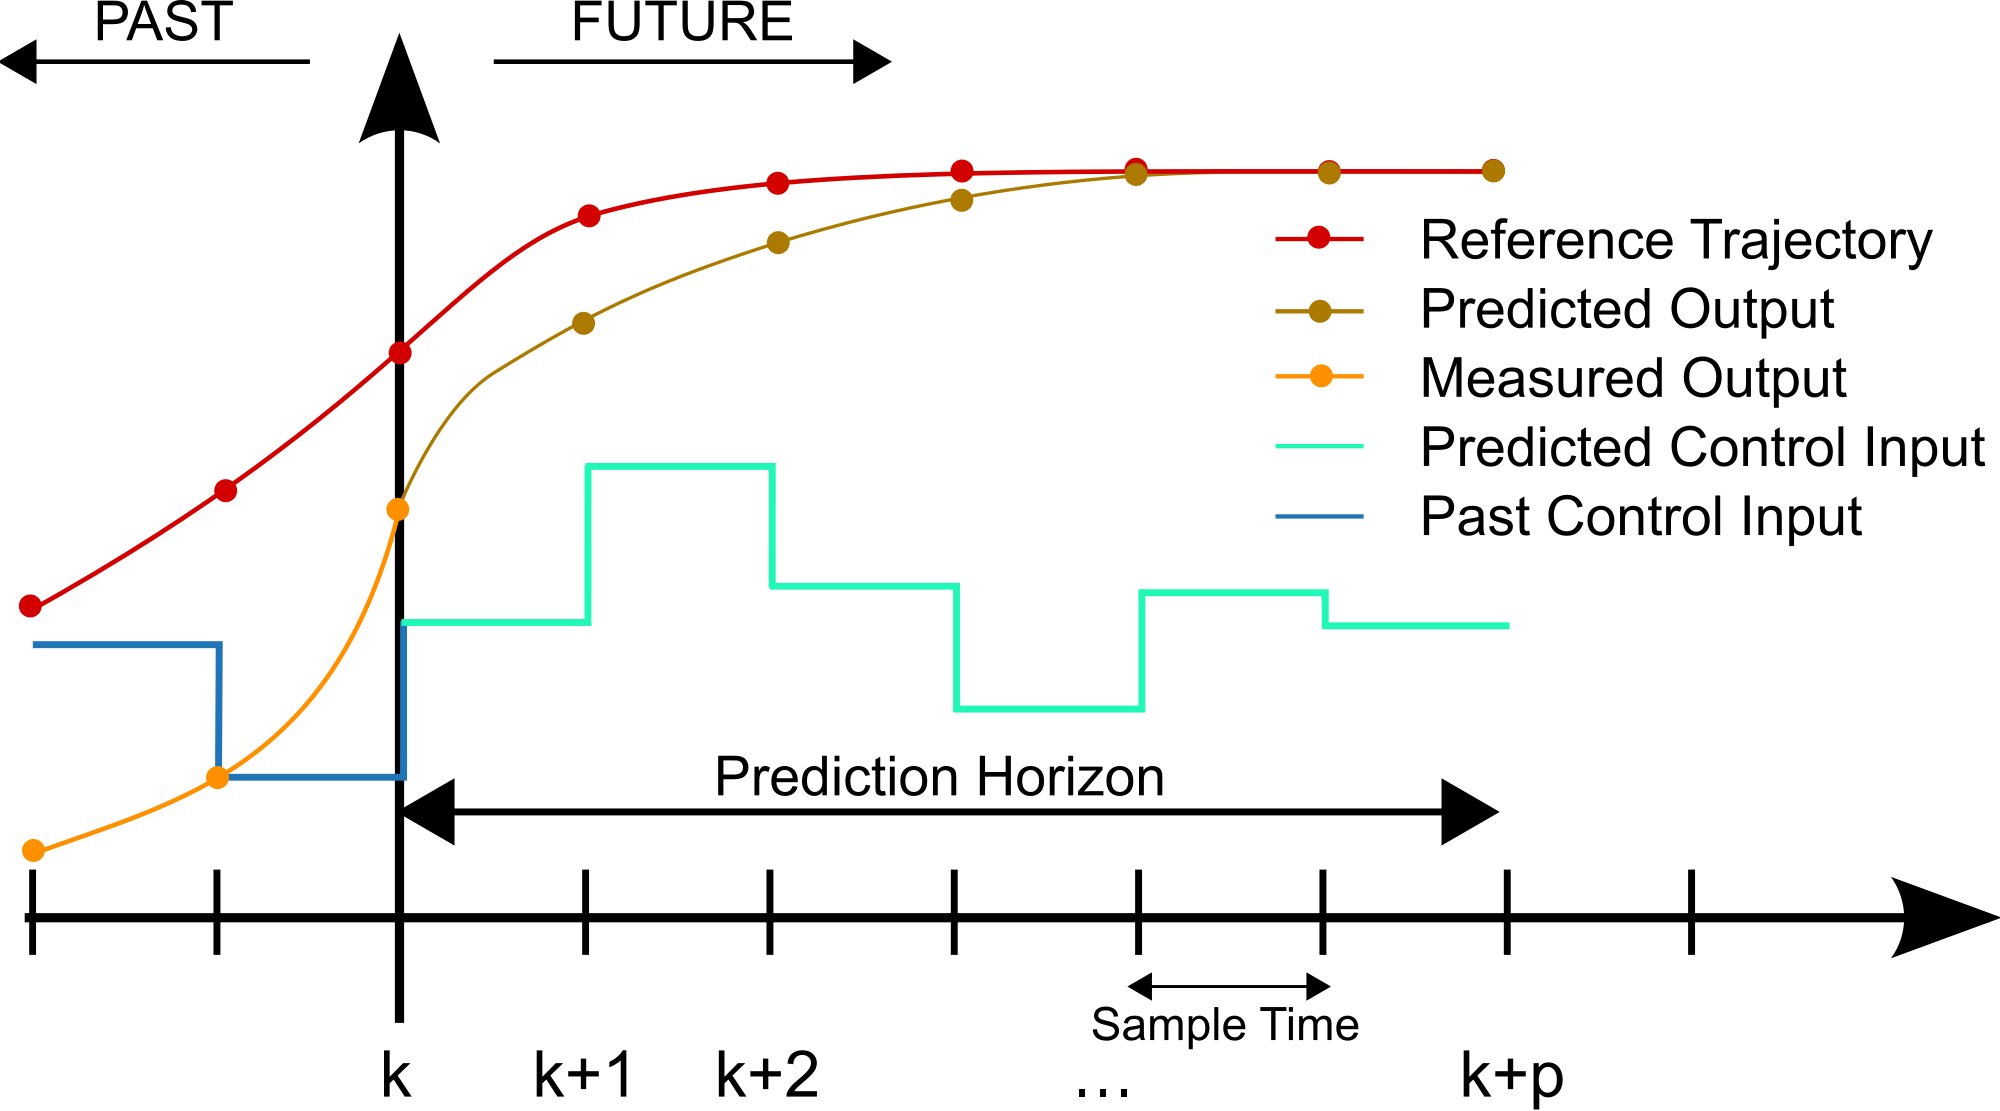
\includegraphics[scale=0.15]{MPC.png}
    \caption{MPC}
    \label{fig:mpc_chart}
\end{figure}

\subsubsection{Sliding Mode Control}
\label{sub:sliding_mode_control}
As mentioned previously sliding-mode control (SMC) is an algorithm for controlling the position of a pneumatic cylinder by directly switching four on/off solenoid valves. SMC is used to provide superior performance in terms of valve switches per second (SPS), steady state error (SSE), settling time and overshoot. These valves are much less expensive than the proportional/servo style valves, however, have a discontinuous flow behaviour making smooth and precise position control more difficult to achieve. While PWM may be used with on/off valves to approximate proportional valves, this frequent switching reduced the lifetime of the valve \cite{zhang_bone_2018}. \newline
This algorithm known as SMC or three-mode sliding mode control (SMC3) can be extended to operate with seven regions of control (SMC7), with the goal of reducing the number of valve SPS. The mode producing the larger acceleration should be chosen since it will reduce the tracking error faster. By adding integral action to these existing algorithms, a reduced settling time and SSE can be achieved if properly applied. Furthermore, by bounding this integral action anti-windup is achieved reducing overshoot and settling time. These extended controllers are referred to as ISMC3 and ISMC7 and can reduce the SPS by up to 37\% when compared to the original SMC implementation whilst maintaining the position tracking error \cite{zhang_bone_2018}.

\subsection{System Modelling}
\label{sub:system_modelling}
The modelling of a multi-variable system allows present input values to predict future values of the output. This can be combined with real world system measurements to accurately create an error signal proportional to the system error. A muscle model can be divided into two main parts, mechanical and pneumatic, a model can be described in terms of its static relationships between forces using methods such as finite element analysis or virtual work relationships. These models can be extended by considering more complex dynamic characteristics of the system.

\subsubsection{Static Modelling}
\label{sub:static_modelling}
Most robotic systems driven by PAMs require an underlying torque controller. This can be achieved with only a static force map leading to an accurate, high-performance control scheme. Nevertheless, a model describing the static PAM force precisely is crucial for the accuracy of the torque controller \cite{martens_boblan_2017}. Several fundamental models for PAM have been proposed to this date aimed at describing the static characteristics of PAM, approaches include functions based on energy conservation assuming the ideal cylinder nature of the muscle. These form simplified static models considering some simple structural parameters. These lumped parameter models account for the pneumatic circuit pressure and mass flow \cite{chou_hannaford_1996}. Other methods used to determine static characteristics use the isobaric, isotonic and isometric nature of a pressure dependant system. Isotonic characteristics determine the muscle length when the load is constant and there are changes in internal pressure. The isometric condition occurs when controlling the internal pressure to achieve constant contraction with a varying load. Lastly the isobaric characteristics corresponding to an axial contraction with constant pressure and a varying load \cite{takosoglu_laski_blasiak_bracha_pietrala_2016}. These principles can be used to determine formulae defining the minimum, maximum and relative static contraction. \newline

\begin{figure}[!hbt]
    \centering
    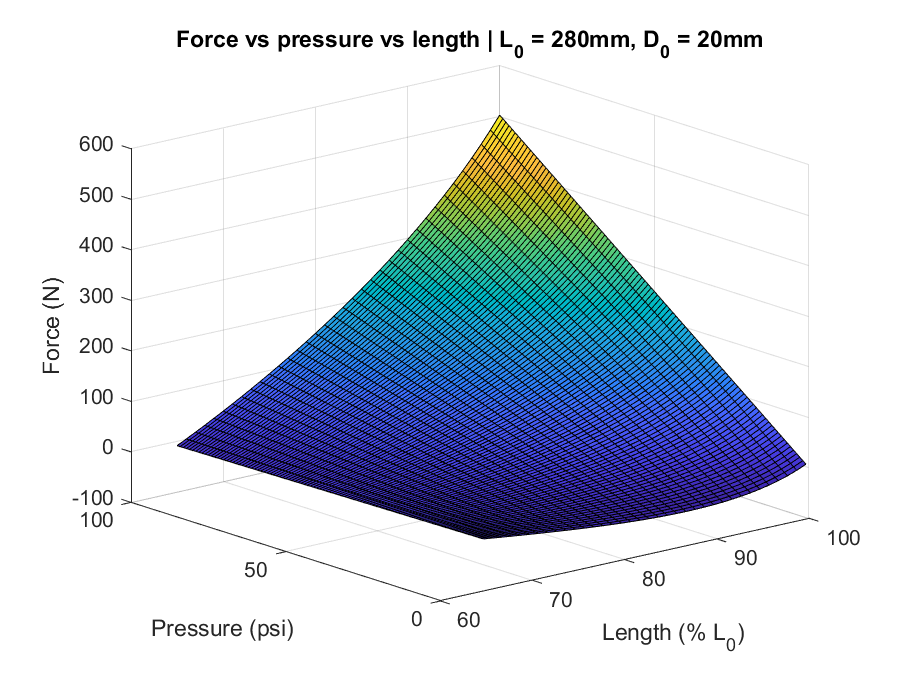
\includegraphics[scale=0.8]{staticmap.eps}
    \caption{Force vs. pressure vs. length with initial length 280mm and diameter 20mm}
    \label{fig:staticmap}
\end{figure}

By considering the behaviour as both a pressure dependant system and as a mechanical spring with some varying stiffness, one can determine a physically motivated model that is closer to the measure force characteristic of a PAM than any existing model. The idea is the approximation of a PAM as a piston with a virtual, pressure dependent piston area and a spring that counteracts the expansion. This approach has been compared to existing models resulting in the maximum error between the previous and new models of 4.4\% \cite{martens_boblan_2017}. This model can be represented by a 3D static force map \Cref{fig:staticmap} as a function of the pressure internal to the system and the length or contraction percentage. As seen in \Cref{math:staticforce} the force generated is only dependent on the work done by the volume of air and the elasticity of the membrane, see \Cref{sub:staticforcederive} for the derivation.

% \begin{figure}[!hbt]
%     \centering
%     \begin{tikzpicture}[scale = 0.5]
%         mass/.style={draw,thick},
%         spring/.style={thick,decorate,decoration={zigzag,pre length=0.3cm,post
%         length=0.3cm,segment length=6}},
%         ground/.style={fill,pattern=north east lines,draw=none,minimum
%         width=0.75cm,minimum height=0.3cm},
%         dampic/.pic={\fill[white] (-0.1,-0.3) rectangle (0.3,0.3);
%         \draw (-0.3,0.3) -| (0.3,-0.3) -- (-0.3,-0.3);
%         \draw[line width=1mm] (-0.1,-0.3) -- (-0.1,0.3);}]
        
%         \begin{scope}[shift={(20,-12.5)},rotate=90]
%             \draw (1,5) -- (1,19) -- (5,19) -- (5,5) -- (1,5);
%             \draw (0,17) -- (1,17) coordinate[pos=0](UpperConnection);
%             \draw (0,6) -- (1,6) coordinate[pos=0](LowerConnection);
%             \filldraw (1,15) rectangle (5,16);
%             \filldraw[fill=white] (2.9,15) rectangle (3.1,1);
%         \end{scope}
        
%          % Left Wall
%         \node[ground,minimum width=3mm,minimum height=2.5cm] (g1){};
%         \draw (g1.north east) -- (g1.south east);
%         % \draw[spring] ([yshift=3mm]g1.east) coordinate(aux) -- (m1.west|-aux) node[midway,above=1mm]{$F_{S1}$};
        
%     \end{tikzpicture}
%     \caption{Caption}
%     \label{fig:my_label}
% \end{figure}

\begin{equation}
F_{PMA}(\rho, l) = -\rho.\frac{dV}{dL}+F_{PE}.\frac{dD}{dL}-F_L
\label{math:staticforce}
\end{equation}

\subsubsection{Dynamic Modelling}
\label{sub:dynamic_modelling}
Pneumatic air muscles have their own dynamics, like hysteresis, some thermodynamic effects and can even be interpreted as a mass spring damper combination \cite{martens_boblan_2017}. Models dependent on the construction parameter and air pressure have been developed providing a tensile force formula of the contractor actuator and can be modified to describe the extension force. One model based on a combination of sigmoid functions representing the force output as a function of both the air pressure and initial length, is an estimation derived from three experimental results over varying lengths. This model assumes an average extension ratio of 50\%, the perfect cylindrical shape with zero wall thickness of the inner bladder, constant friction-less contact between the braid and inner tube, constant braid strand length and elasticity of the rubber tube. This model lacks an accurate description of the complex non-cylindrical shape at low pressures and the imperfect contact between the inner tube and braided sleeve \cite{al-ibadi_nefti-meziani_davis_2018}. \newline

Extending this, the problem can be approached as a mechanically derived nonlinear spring, the stiffness of which can be controlled by the muscle pressure. This relationship can be depicted by a fifth order polynomial of two variables of twenty-one coefficients. The pneumatic part of the model is divided into two main components, the model of volume flow rate through the valves and a differential equation for the muscle pressure. The use of on/off style solenoid valves simplifies the flow rate to either a constant compressor pressure or atmospheric pressure, solely dependent on the muscle pressure. The second pneumatic component is the derivative time dependent equation derived from ideal gas laws. This research found that the hysteresis effects of the muscle actuator cause some steady state error due to simplified descriptions of the mechanical force components. Refinement of the model could decrease the errors to reduce the reliance on the robustness of the control technique \cite{hosovsky_2012}. Below is the equation found representing these forces \Cref{math:dynamicforce}, where m - moving mass (kg), y - muscle displacement (m), F\textsubscript{S}(k,P\textsubscript{m}) - nonlinear term representing a variable spring force (N), F\textsubscript{D}(\.{k},P\textsubscript{m}) - nonlinear term representing a variable damper force (N), F\textsubscript{E} - external force (N), k - muscle contraction (defined as k = k\textsubscript{0} + y/l\textsubscript{0} where k\textsubscript{0} is the initial contraction and l\textsubscript{0} is the initial muscle length (-) and P\textsubscript{m} - the absolute muscle pressure (Pa).

\begin{equation}
    \ddot{y} = \frac{1}{m}[F_E-F_S(k,P_m)-F_D(\dot{k},P_m)]
    \label{math:dynamicforce}
\end{equation}

\clearpage
\section{System Implementation and Electronics}
\label{sec:system_implementation}

The following section outlines the ultimate goal of the project describing a platform design that should more closely mimic a human. A test rig has been developed to assess the success of pneumatic muscles as an actuator.

\subsection{Platform Design}
\label{sub:platform_design}

The ultimate goal of this design, dubbed PNEUbot, will be to develop a humanoid robotic platform designed to replicate the motions of a human closer than the current electric servo driven humanoid robots. To achieve this goal an alternate actuator must be developed, and a platform feasibility study performed to determine the viability of the actuator developed. \Cref{fig:platform} shows how this platform has been conceptually designed to mimic the range of joint movements capable of a human. This biologically inspired platform is formed around the skeleton dimensions of an adult human, implementing muscle groups to control the joints for each degree of freedom. As an alternate actuator, pneumatic muscles have a limited contraction of 25-30\% when compared to the 50-70\% stroke of a human muscle, design constraints needed to be placed on some DoF joints for the range of motion available for that joint due to this reduced contraction. Consequently, due to the force curve produced by pneumatic muscles, the force capable of being produced at the end of a muscle stroke is limited by its physical parameters. The ultimate project specifically aims to design and construct a knee and ankle joint for a single leg, this will form the basis for the platform.\newline

The current world class strictly humanoid robotic platform was designed by a German team from the University of Bonn. This platform stands 135cm tall, weighs 18kg and has 18 DoF: 5 per leg (parallel kinematics), 3 per arm and 2 in the neck \cite{ficht_farazi_brandenburger_rodriguez_pavlichenko_allgeuer_hosseini_behnke_2018}. These servos can produce 12.9 N.m of stall torque with a maximum of 37 rpm at no load at a 12-bit resolution \cite{robotis}. For this overall project, this platform will be the benchmark for the use of pneumatic air muscles as an alternate actuator. \newline

\begin{figure}[!hbt]
    \centering
    \begin{subfigure}[t]{0.4 \textwidth}
        \centering
        \caption{Side Profile}
        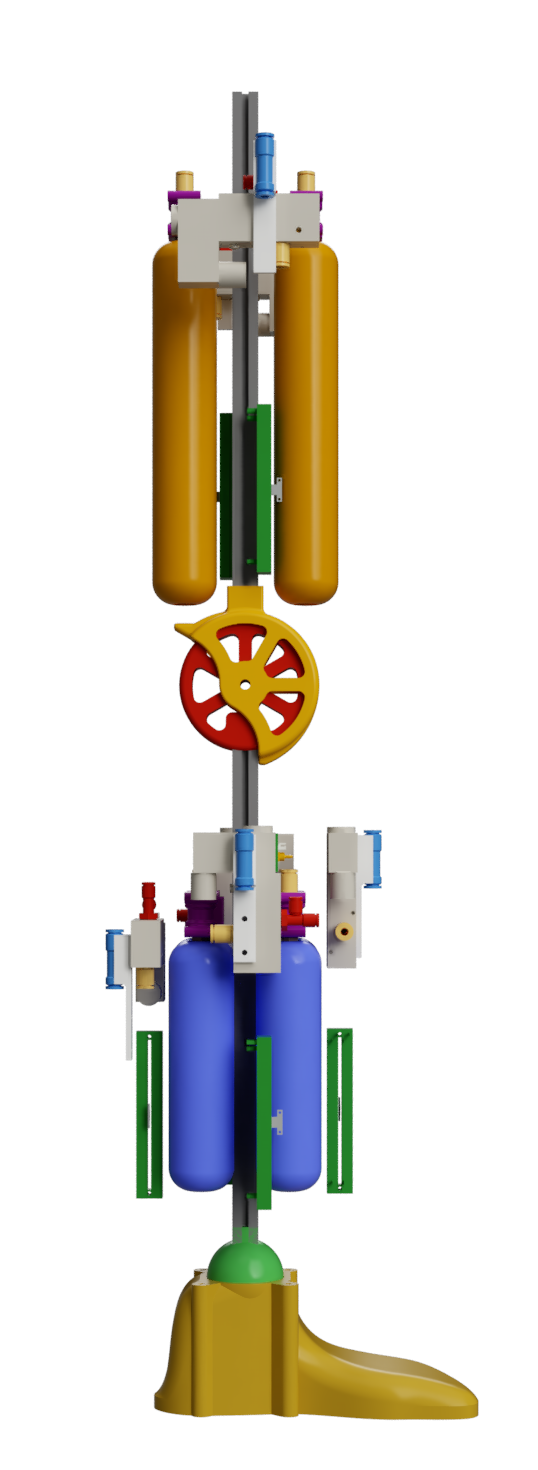
\includegraphics[scale=0.2]{Leg_Render_Side_2.PNG}
        \label{fig:platform_side}
    \end{subfigure}
    \begin{subfigure}[t]{0.4 \textwidth}
        \centering
        \caption{Design Concept}
        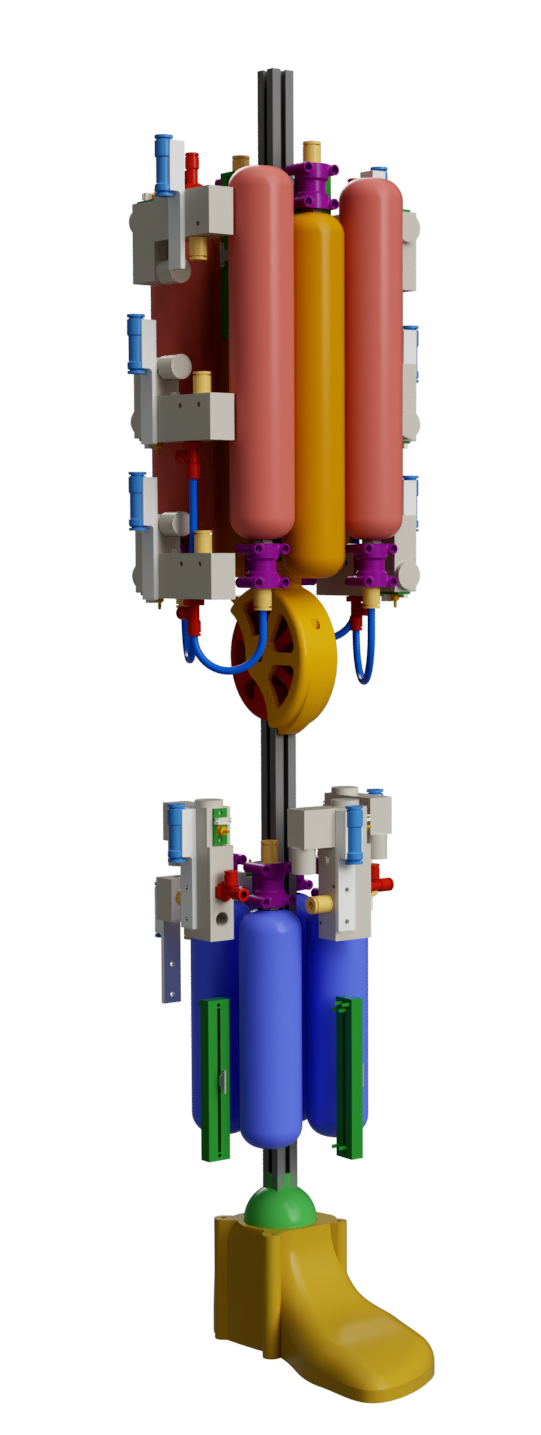
\includegraphics[scale=0.2]{Leg_Render.PNG}
        \label{fig:platform_angle}
    \end{subfigure}
    
    \definecolor{blue_m}{RGB}{83, 106, 212}
    \definecolor{mustard_m}{RGB}{200, 119, 109}
    \definecolor{sausage_m}{RGB}{197, 140, 18}
    \begin{tikzpicture}[show background rectangle,inner frame sep=2mm, scale=0.5]
        \node [fill=blue_m, rounded corners, inner sep=0.3cm, draw, thick] (A) {};
        \node [right = 0.2cm of A] (A_text) {Ankle};
        \node [right = 1cm of A_text, fill=mustard_m, rounded corners, inner sep=0.3cm, draw, thick] (B) {};
        \node [right = 0.2cm of B] (B_text) {Hip};
        \node [right = 1cm of B_text, fill=sausage_m, rounded corners, inner sep=0.3cm, draw, thick] (C) {};
        \node [right = 0.2cm of C] (C_text) {Knee};
    \end{tikzpicture}
    \caption{PNEUbot Robotic Platform Concept Design}
    \label{fig:platform}
\end{figure}

\subsubsection{Leg Design}
\label{subsubsection:leg_design}

To achieve a lightweight skeleton the robot will be constructed from aluminium extrusion 'bones', 3D printed mounts and protective covers. Bearings will be inserted into the knee joint, with a spherical ball joint forming the ankle pivot. High tensile nylon line will act as tendons providing the transmission of the pneumatic muscle force to the actuated joint. \newline

The knee joint will consist of a pair of muscles acting as the flexion and extension muscles. These will be placed on the upper leg area of the robot producing approximately 120$^{\circ}$ of motion. To achieve the 2 DoF dorsiflexion/plantar flexion and eversion/inversion of the ankle, 2 pairs of coupled muscle actuators will be placed around the lower leg. These muscles will be coupled as opposed to decoupled to provide a parallel actuation force for the plantar flexion of the ankle joint. This should theoretically reduce the force required from each muscle whilst also reducing the physical size of the lower leg. 

\subsubsection{Test Rig}
\label{subsubsection:Test Rig}
The focus of this stage of the project is to develop a software framework that can be utilised in the control of the pneumatic muscles. A test rig, \Cref{fig:test_rig}, has been designed that replicates the motion of the single degree of freedom knee joint proposed in the leg design. It consists of two identical counteracting muscles which are connected to a pivot via a nylon line. To simulate the range of rotational movement of a knee, approximately 120$^{\circ}$, the contraction length of the muscles must match the arc length of the segment formed by the 120$^{\circ}$ pivot. And thus the radius and contraction length are proportional by \Cref{math:arc_length}. 

\begin{equation}
    Length = \Theta r
    \label{math:arc_length}
\end{equation}

The muscle length was chosen to fit within the constraints of the upper leg portion of the leg design. A resting muscle length of 280 mm results in a contraction length of approximately 100 mm. This can be used to find the radius of 47.7 mm for a 120$^{\circ}$ segment. 
The rig allows the addition of variable mass to the rotating arm to test the control structures response in varying conditions. The pivot disc allows the muscles to rotate around a 94mm diameter increasing the torque capable of being produced whilst maintaining adequate range of motion.
If more torque was required for the joint, many parameters of the system could be changed to alter the performance. As \Cref{math:staticforce} shows, the force produced by the muscle is dependent on the diameter, length and pressure of the muscle.

\begin{figure}[!hbt]
    \centering
    \begin{subfigure}[t]{0.95 \textwidth}
        \centering
        \caption{Test Rig}
        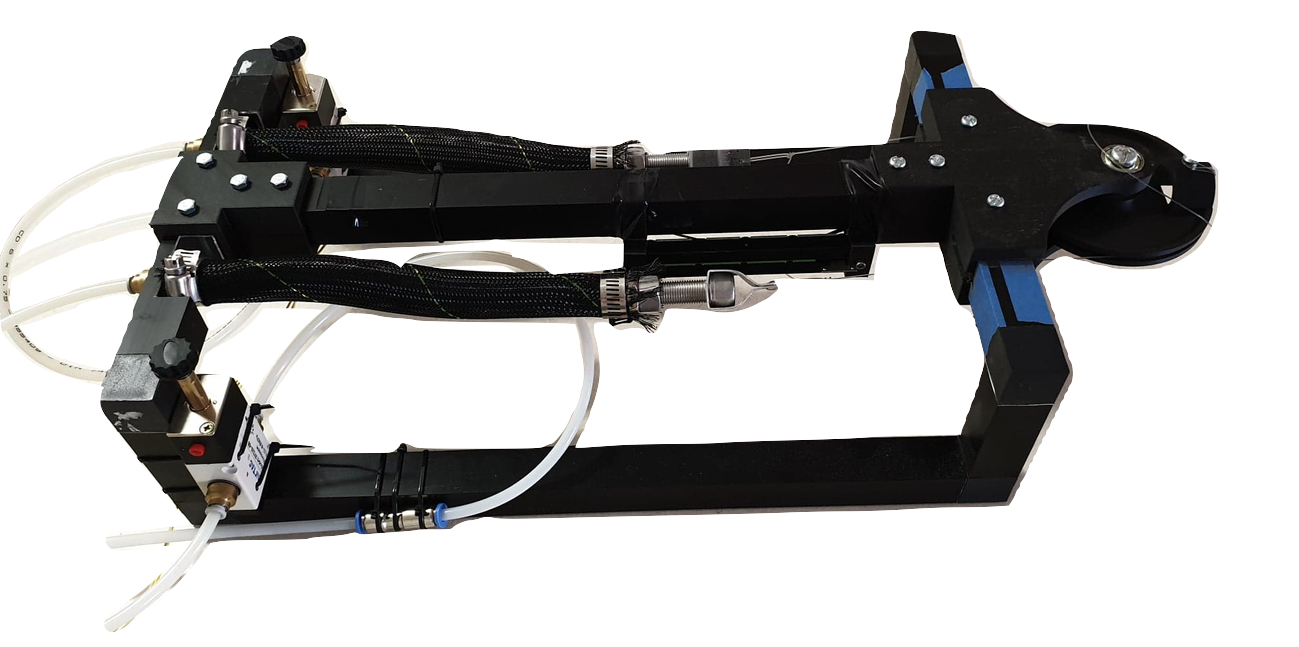
\includegraphics[scale=0.2]{Test_Rig_Photo.png}
        \label{fig:test_rig_photo}
    \end{subfigure}\\
    \begin{subfigure}[t]{0.45 \textwidth}
        \centering
        \caption{Design Concept Top View}
        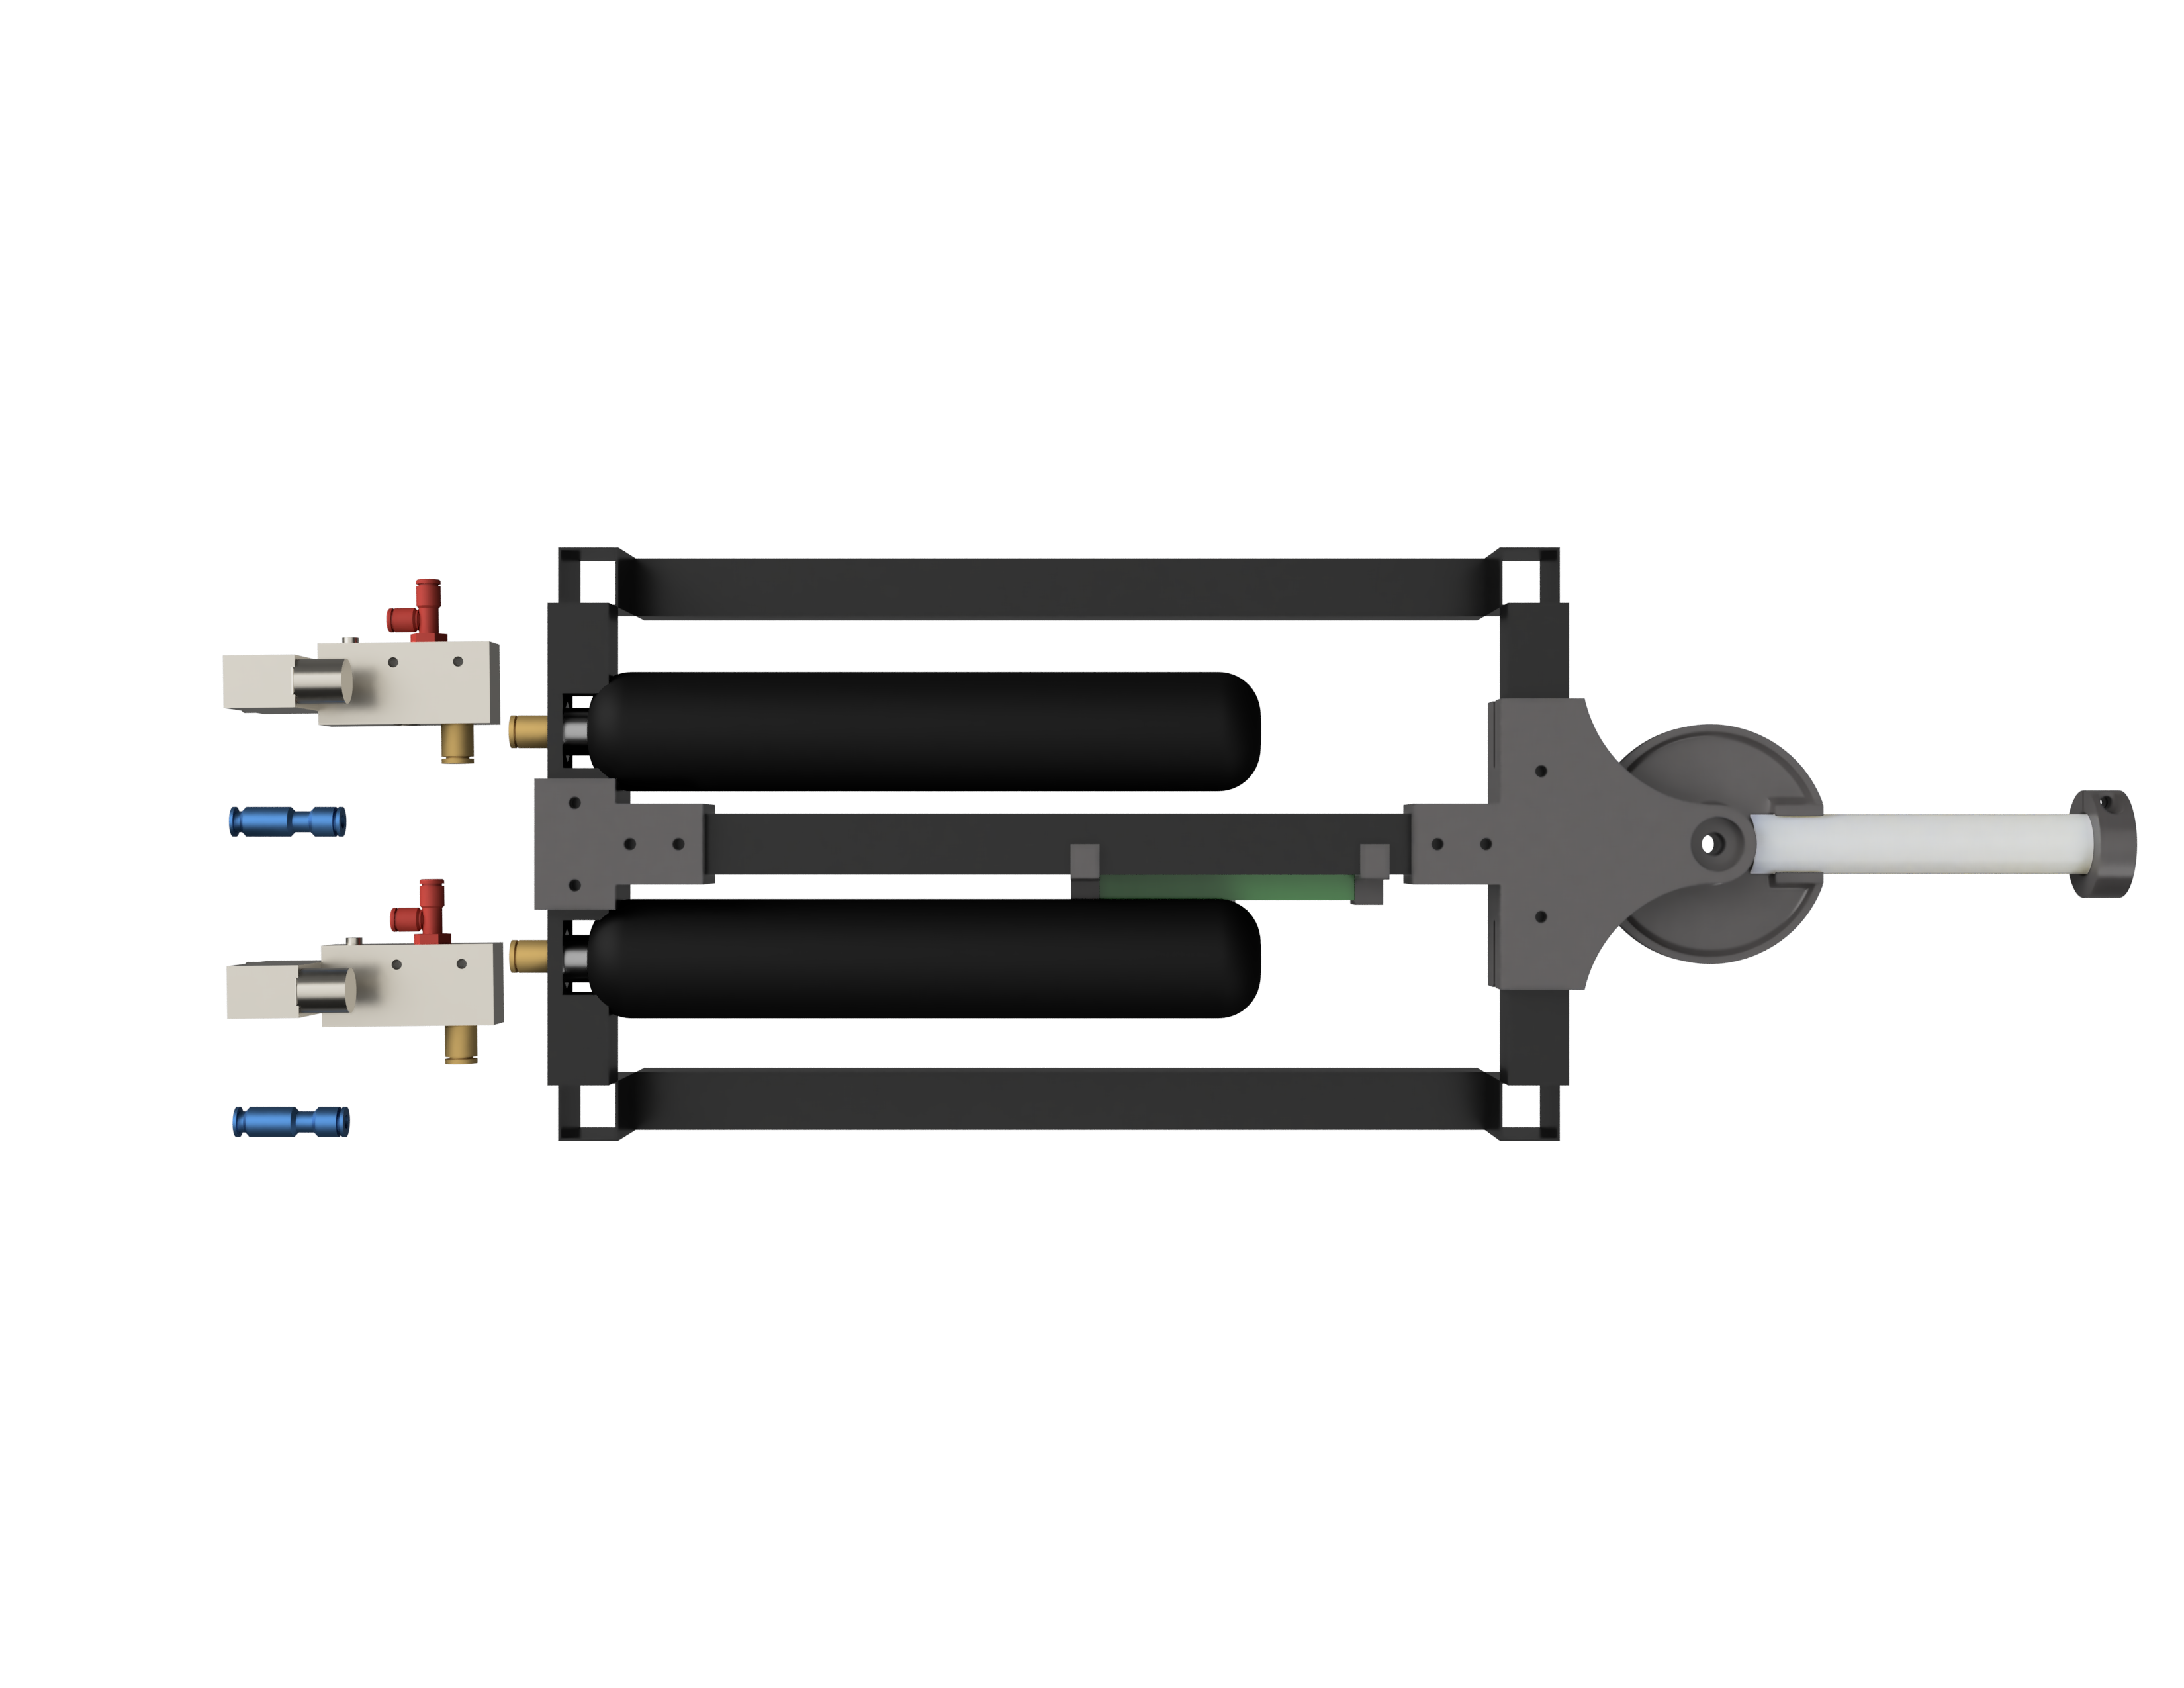
\includegraphics[height=6cm, trim={1cm 2cm 1cm 1cm},clip]{Testrig_top.PNG}
        \label{fig:test_rig_design_top}
    \end{subfigure}
    \begin{subfigure}[t]{0.45 \textwidth}
        \centering
        \caption{Design Concept}
        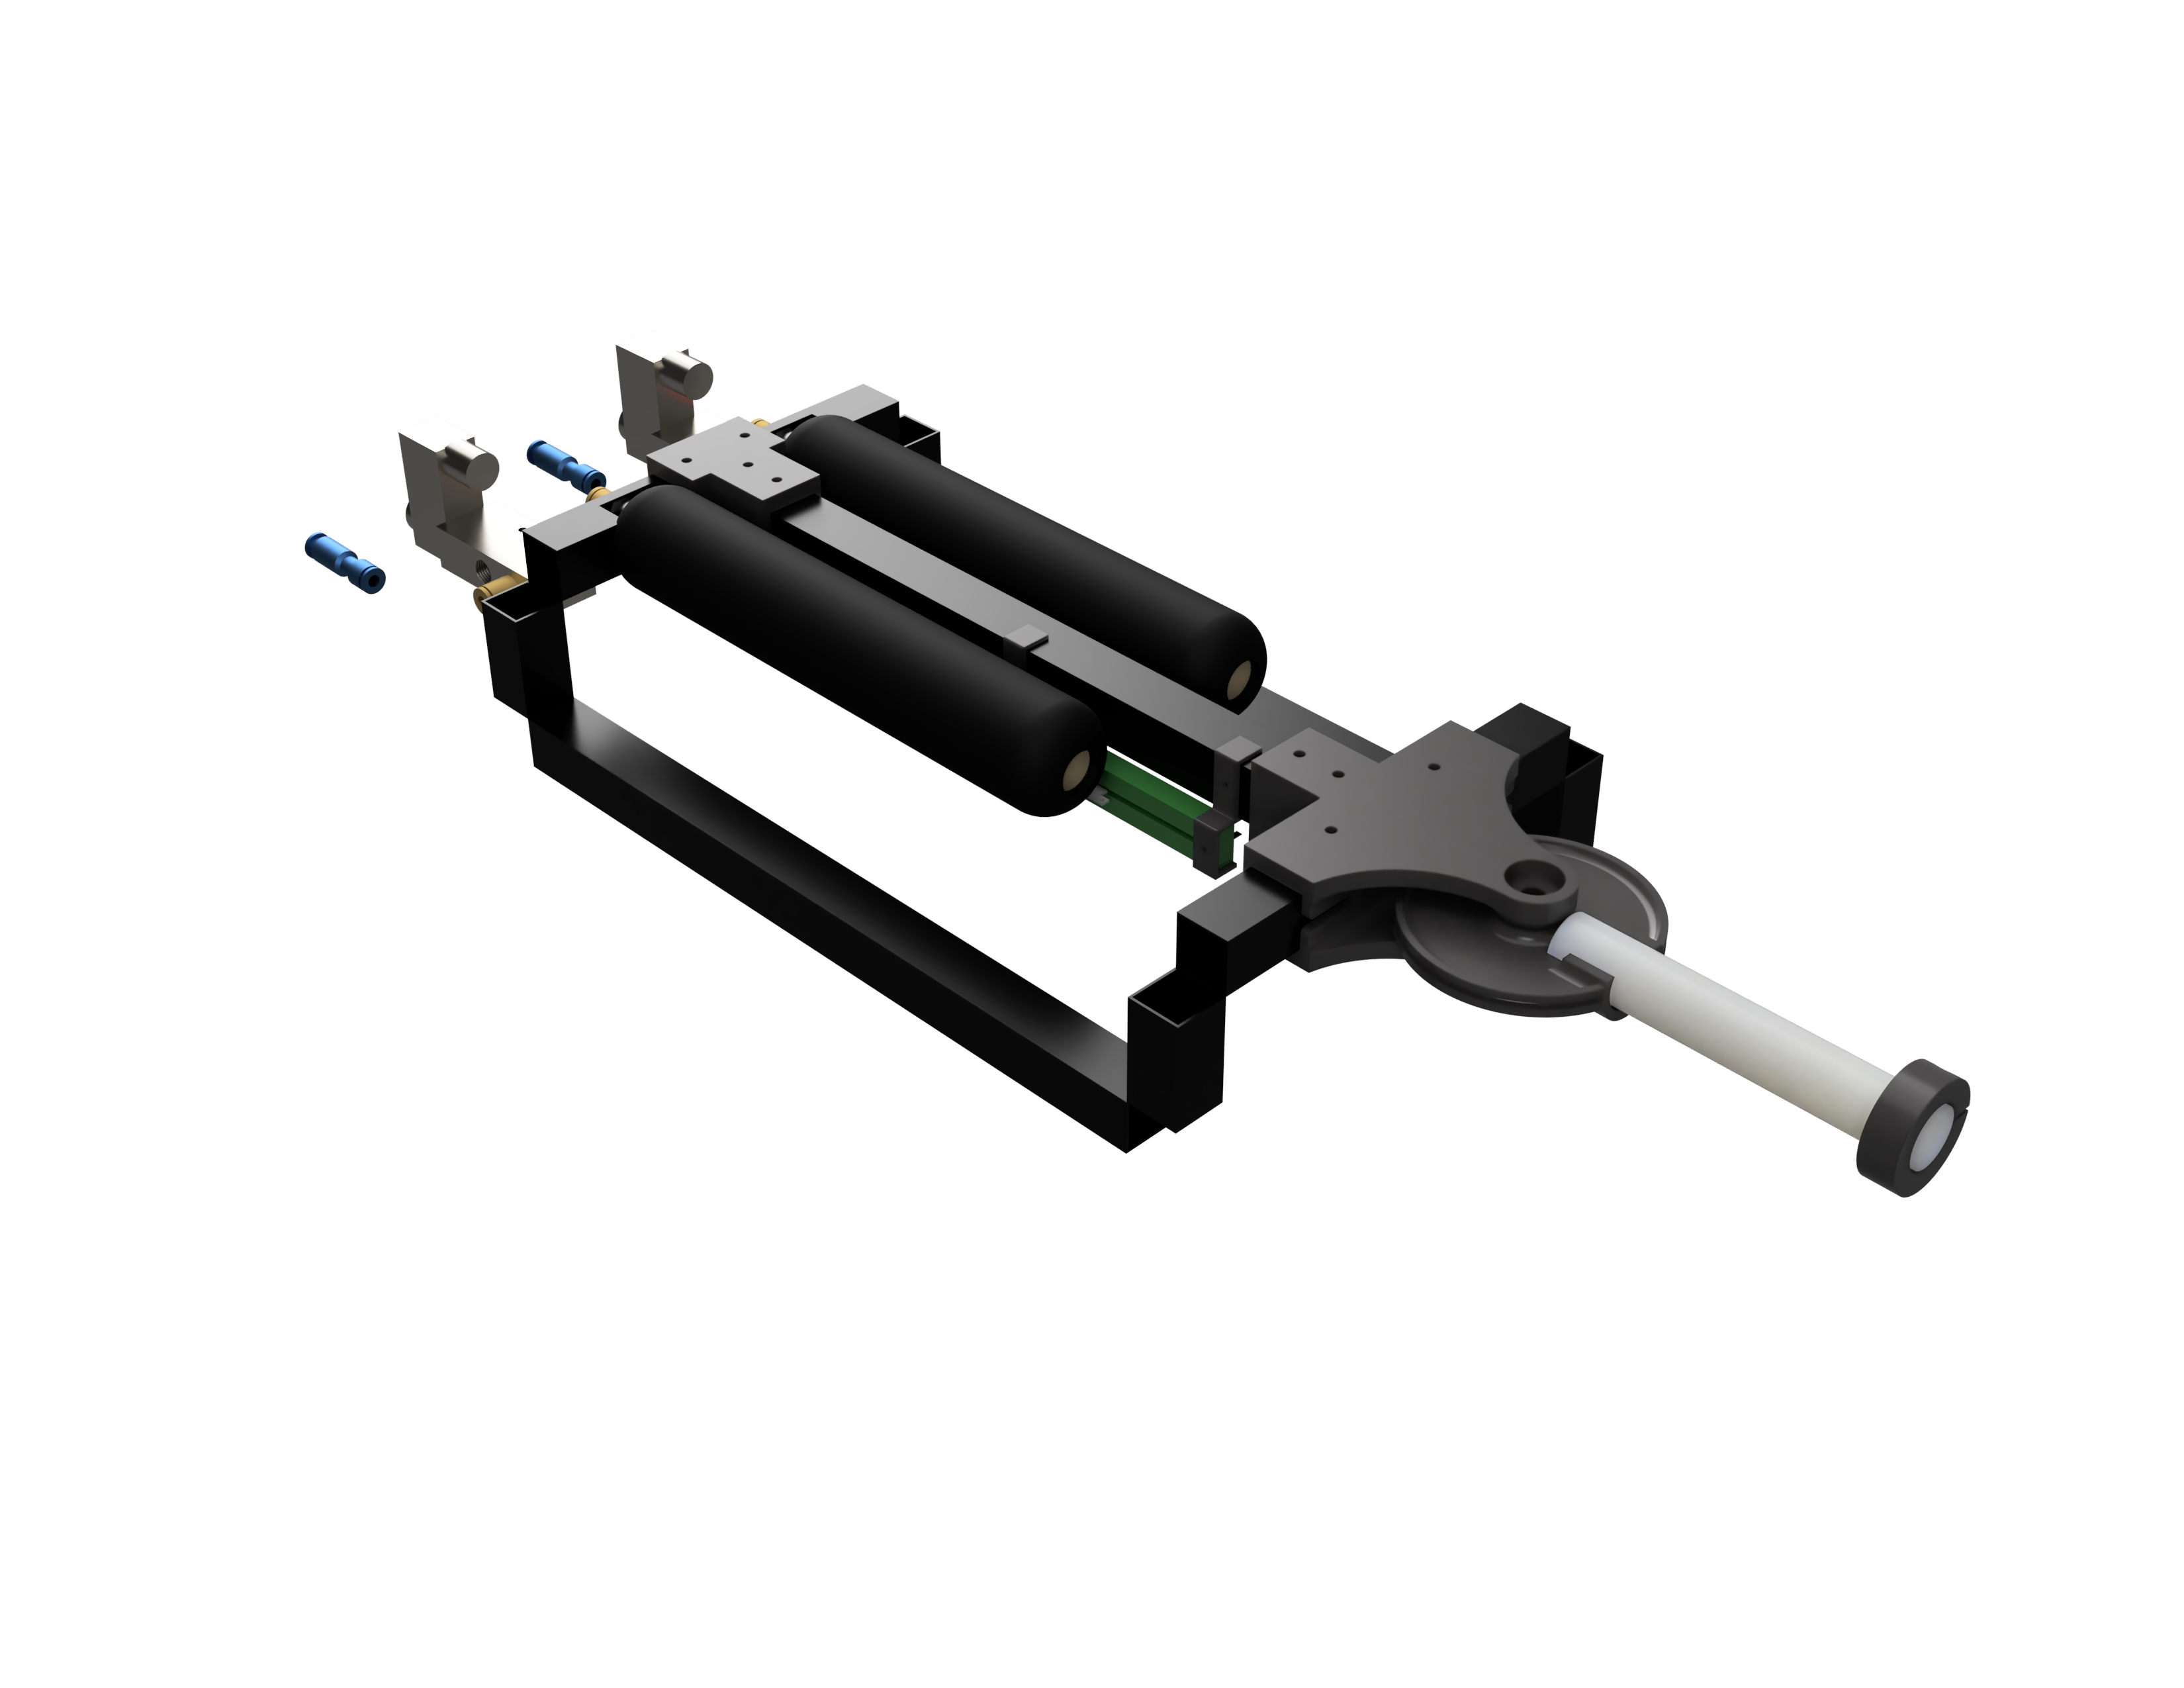
\includegraphics[height=6cm, trim={1cm 2cm 1cm 1cm},clip]{Testrig_home.PNG}
        \label{fig:test_rig_design}
    \end{subfigure}
    \caption{1 DoF Test Rig}
    \label{fig:test_rig}
\end{figure}


\subsection{Muscle Construction and Control}
\label{sub:muscle_construction}

The following section describes the pneumatic muscle design and construction with the goal of finding a compatible set of materials for the two major items. Furthermore, the pneumatic system design and construction is also detailed.

\subsubsection{Muscle Design}
\label{subsubsection:muscle_design}
The pneumatic muscles are constructed from two major components, the inner airtight bladder and the outer braided mesh. As these two components must be chosen to be 'compatible' with each other, a series of experimental trials were performed to determine suitable components. A combination of two bladder materials, each with two diameters was trailed against two braid diameters. The bladder materials selected were a natural latex and a silicone tube. The two bladder diameters selected were 6 mm ID, 9 mm OD and 10 mm ID, 14 mm OD. As for the braid, diameters of 20 and 40 mm were tested. This selection of components was selected due to the availability of products and cost. A variety of muscles were constructed and tested for load lifting capability and reliability. After repeated tests it was found that the selection of bladder and braids were incompatible. This incompatibility was evident in the non-uniform expansion of the bladder, resulting in decompression of the muscle bladder. \newline

A final bladder material and diameter was experimentally trailed with the original two braids. An 18 mm ID, 22 mm OD road bike tube was used to construct a 280 mm length muscle. The muscle utilising the larger diameter braid failed longitudinally along the bladder, whilst the smaller braid successfully performed in repeated trials. This muscle was capable of lifting up to 16 kg whilst maintaining full contraction.\newline
The conclusion of this experiment is that compatibility of muscles means the diameters of the two components should be as close as possible. As the difference between the diameter of the bladder and the braid increases, the inflation of the muscle can become irregular. This can cause uneven stresses and pressures on the inside of the bladder leading to premature failure. Failure can occur in one of two ways. The bladder can form 'rings' \Cref{fig:incompatible_rings} around the circumference of the material, this non-uniform expansion results in increased pressure on parts of the bladder causing failure. The second failure occurs when the non-uniform expansion occurs laterally down the bladder. \Cref{fig:incompatible_banana} shows the 'banana' shape when one side of the braid contracts prematurely which can also result in failure. Both of these failures were seen in testing when the resting diameters of the two components differed by more than $30\%$ as seen in \Cref{fig:incompatible_muscles}.

\begin{figure}[!hbt]
    \centering
    \centering
    \begin{subfigure}[t]{0.45 \textwidth}
        \centering
        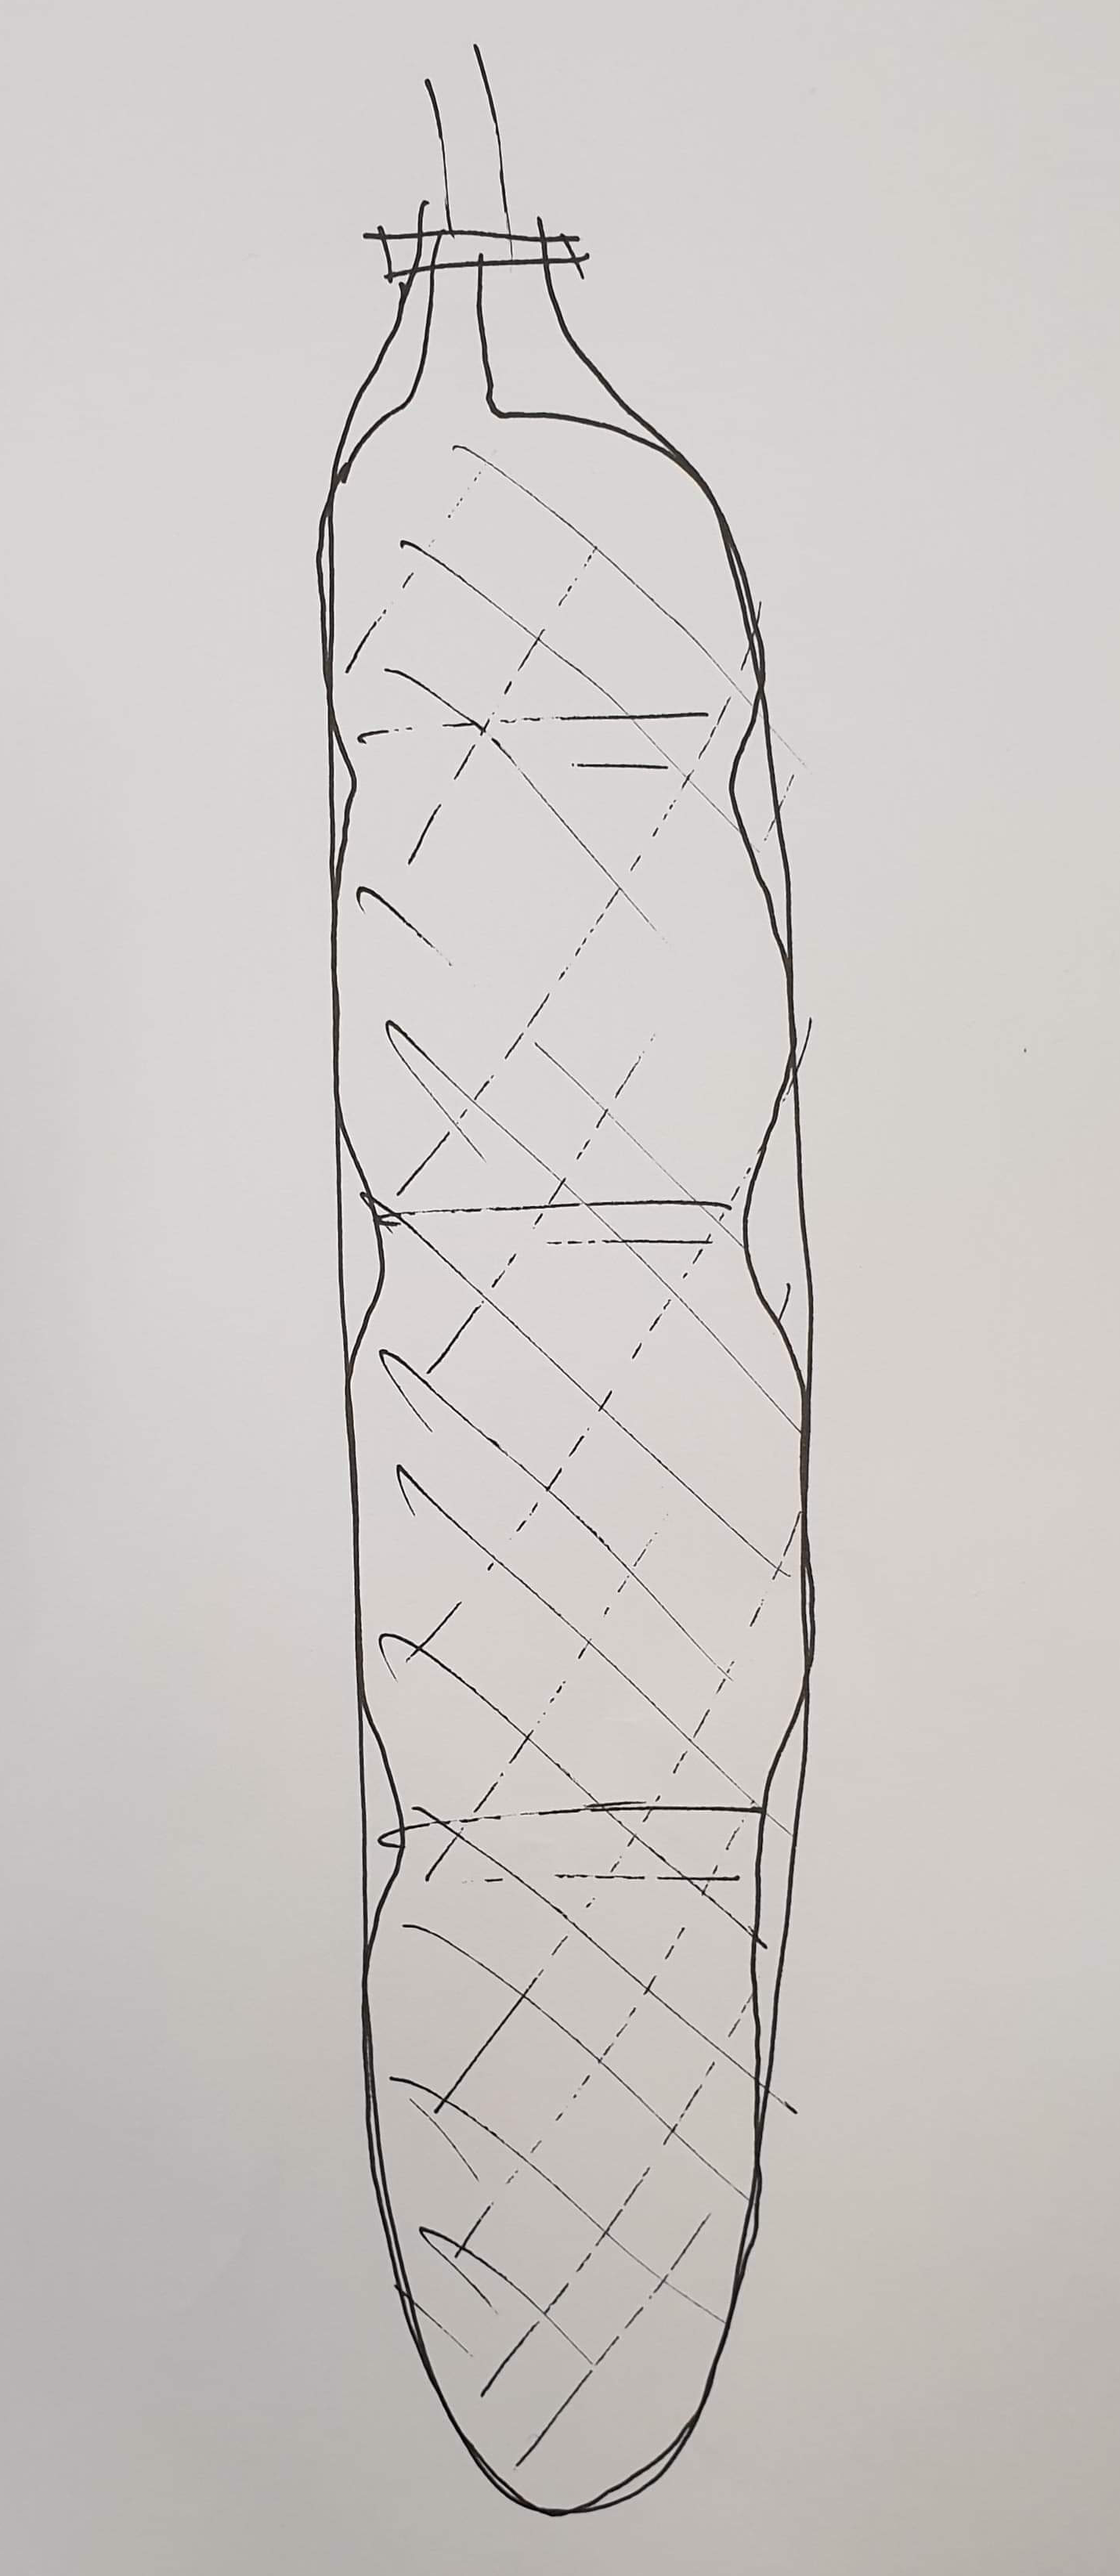
\includegraphics[height=10cm, trim={0cm 60cm 0cm 0cm},clip]{MuscleRinging.png}
        \caption{Muscle Ringing}
        \label{fig:incompatible_rings}
    \end{subfigure}
    \begin{subfigure}[t]{0.45 \textwidth}
        \centering
        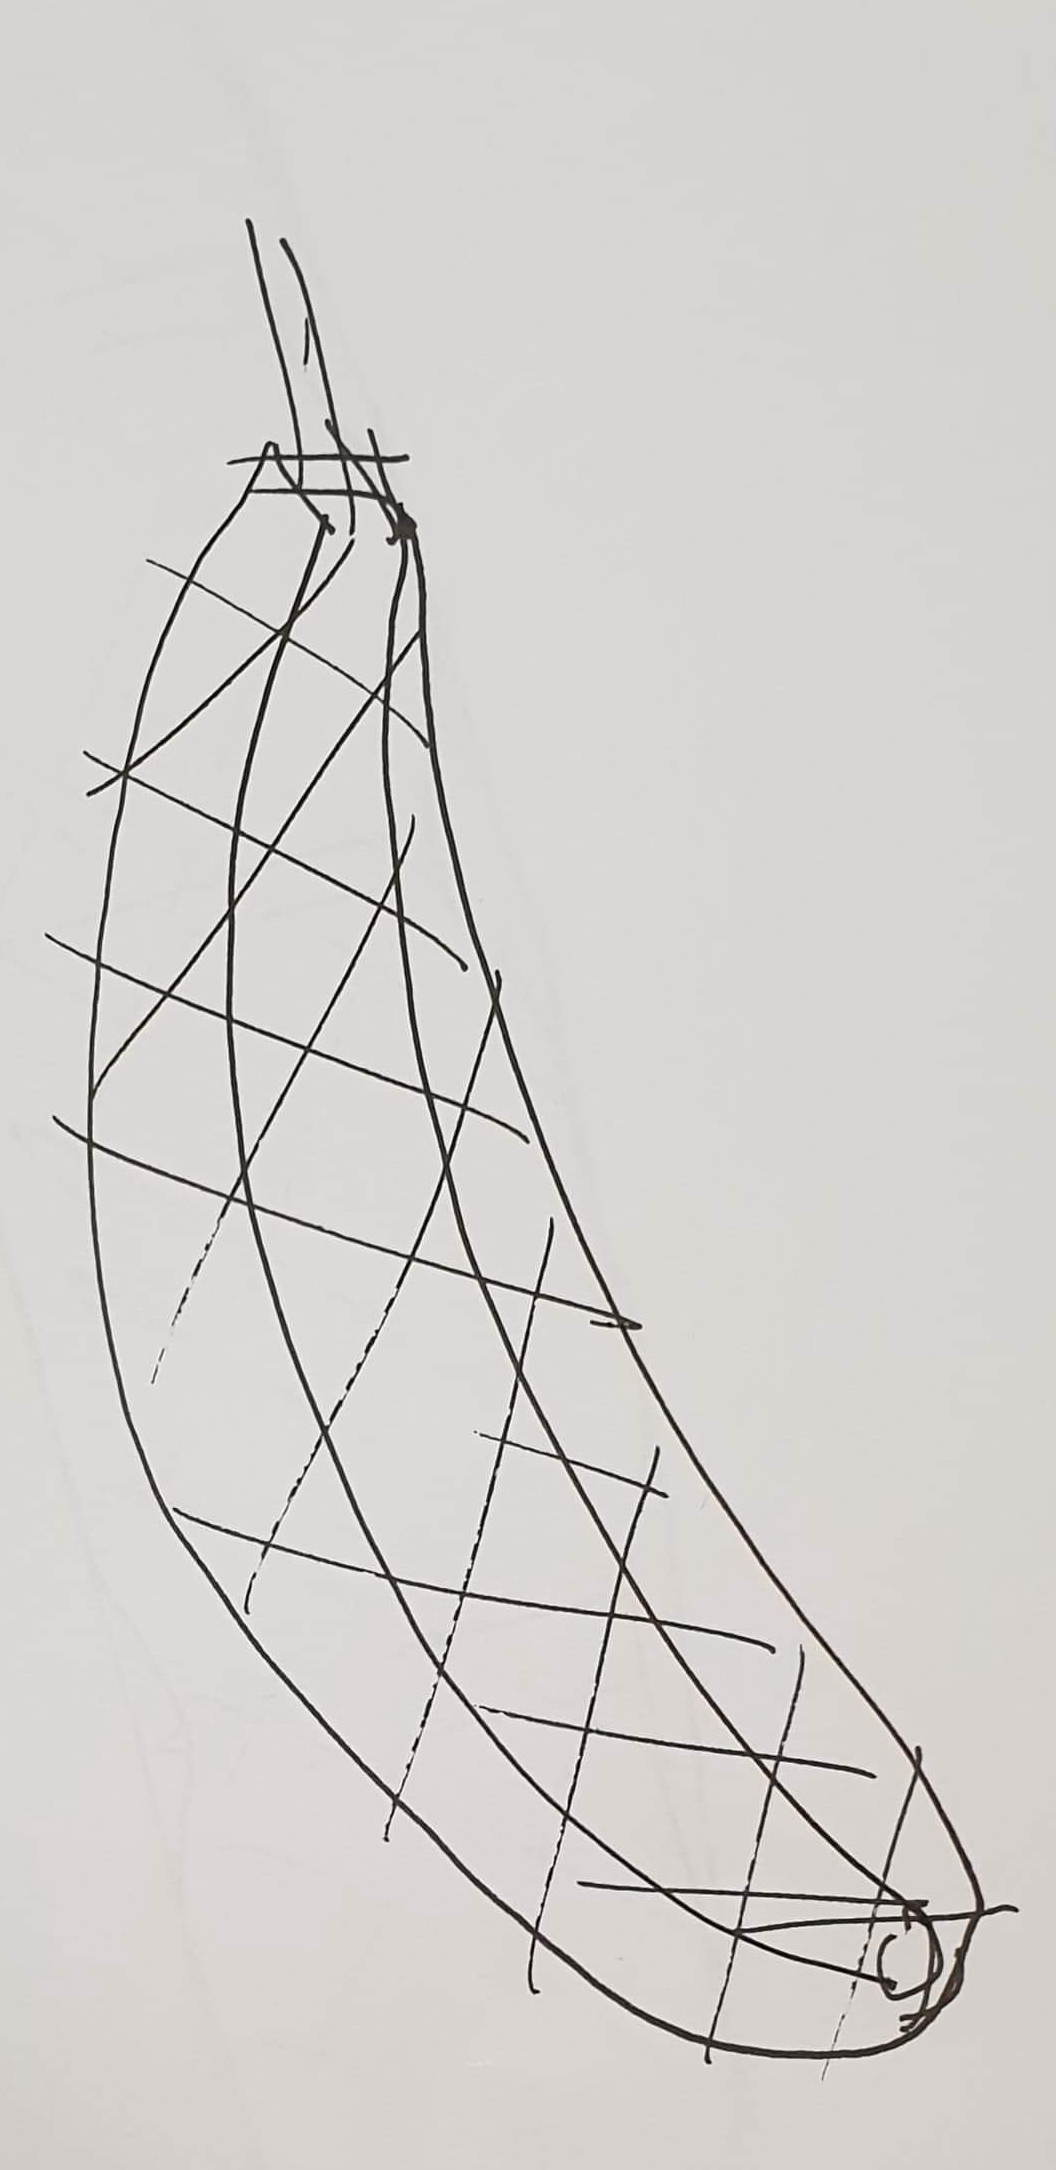
\includegraphics[height=10cm, clip]{MuscleBananaing.png}
        \caption{Muscle Bananaing}
        \label{fig:incompatible_banana}
    \end{subfigure}
    \caption{Muscle Failures}
    \label{fig:incompatible_muscles}
\end{figure}

The final design inner bladder was chosen with an internal diameter of 16mm and wall thickness of 2mm, the specific material used was a road bike tube. The braided mesh of 20mm diameter was selected to be compatible with the bladder diameter as according to the experiments run previously and other literature \cite{andrikopoulos_nikolakopoulos_2017}.

\subsubsection{Pneumatic Control}
\label{subsubsection:pneumatic_control}

In order to control the flow of air into and out of the muscle bladder a 3 port 2-way pneumatic solenoid valve was used in conjunction with a non-return valve \cite{airsky_pneumatic}. These components were assembled as shown in \Cref{fig:pneumatic_valve}. This arrangement allows each muscle to be in 1 of 2 states. One muscle alone isn't overly useful as it only has the ability to actively move in a single direction, a pair of muscles on the other hand can be arranged to generate opposing forces resulting in a more useful motion capability. \newline

\begin{figure}[!hbt]
    \centering
    \scalebox{0.5}{
        \begin{tikzpicture}
            % Left half
            \draw[very thick] (0, 0) rectangle (5, 5);
            \draw[very thick,black,->] (1.25, 0) -- (1.25, 5);
            \draw[very thick,black] (3.75, 0) -- (3.75, 1);
            \draw[very thick,black] (3.25, 1) -- (4.25, 1);
    
            % Right half
            \draw[very thick] (5, 0) rectangle (10, 5);
            \draw[very thick,black,->] (6.75, 5) coordinate (A) -- (8.75, 0) coordinate (R);
            \draw[very thick,black] (6.25, 0) -- (6.25, 1) coordinate (P);
            \draw[very thick,black] (5.75, 1) -- (6.75, 1);
            \draw[very thick,black] (8.75, 0) -- (8.75, -1);
            \draw let \p1=(P), \p2=(A) in (\x1, \y2) node[below] {\Large{A}};
            \draw (P) node[above] {\Large{P}};
            \draw let \p1=(P), \p2=(R) in (\x2, \y1) node[above] {\Large{R}};
    
            % Right coil
            \draw (10, 1.5) -- (10.5, 3.5) -- (11.0, 1.5) -- (11.5, 3.5) -- (12.0, 1.5) -- (12.5, 3.5);
            \draw (0, 6) node[right] {\LARGE{Solenoid Valve}};
    
            % Non-return valve
            \draw let \p1=($(P) - (0, 4)$) in (\p1) circle (1);
            \draw let \p1=($(P) - (1.5, 4)$), \p2=($(P) + (1.5, -4)$), \p3=($(P) - (0, 5.5)$) in (\p1) -- (\p3) -- (\p2);
            \draw let \p1=($(P) - (0, 3)$), \p2=($(P) - (0, 2)$) in (\p1) -- (\p2);
            \draw let \p1=($(P) - (0, 5.5)$), \p2=($(P) - (0, 6.5)$) in (\p1) -- (\p2);
            \draw let \p1=($(P) + (1.5, -4)$) in (\p1) node[right] {\LARGE{Non-return Valve}};
    
            % Muscle
            \coordinate (pole) at (20, -5);
            \foreach \i in {1,...,20}
            {
                \draw[very thick] let \p1=(pole) in (\x1, \y1 + \i * 20) -- (\x1 + 80, \y1 + \i * 20 - 25);
            }
            \draw[very thick] let \p1=(pole) in (\x1, \y1 - 5) rectangle (\x1 + 80, \y1 + 20 * 20);
            \draw let \p1=(pole) in (\x1 + 90, \y1 + 200) node[right] {\LARGE{Pneumatic Air Muscle}};
    
            % Bottom cap
            \draw[very thick] let \p1=(pole) in (\x1 - 10, \y1 - 5) rectangle (\x1 + 90, \y1 - 25);
            \draw[very thick] let \p1=(pole) in (\x1, \y1 - 25) arc (180:360:1.4);
    
            % Top cap
            \draw[very thick] let \p1=(pole) in (\x1 - 10, \y1 + 20 * 20) rectangle (\x1 + 90, \y1 + 20 * 20 + 20);
            \draw[very thick] let \p1=(pole) in (\x1, \y1 + 20 * 20 + 20) arc (180:0:1.4);
            
            % Line from solenoid valve to top of muscle
            \draw[very thick] let \p1=(A), \p2=(pole) in (\x1, \y1)[rounded corners=10pt]{} --
              (\x1, \y2 + 20 * 20 + 100){} --
              (\x2 + 40, \y2 + 20 * 20 + 100){} --
              (\x2 + 40, \y2 + 20 * 20 + 60){};
    
            % Line from non-return valve to solenoid valve
            \draw[very thick] let \p1=($(P) - (0, 2)$) in (\x1, \y1) -- (P);
    
            % Input line
            \draw[very thick] let \p1=($(P) - (0, 6.5)$), \p2=($(P) - (0, 10)$) in (\x1, \y1) -- (\x2, \y2) node[midway,label=right:{\LARGE{Regulated Air In}}]{};
        \end{tikzpicture}
    }
    \caption{Single Muscle Actuator Assembly}
    \label{fig:pneumatic_valve}
\end{figure}

Consider one muscle under no load. When its internal pressure is equal to the regulated system pressure, the muscle will be under full contraction. Releasing the air from the muscle will allow the muscle to extend back to its nominal length. Switching between the two valve states will allow the muscle to contract and release. 
Now consider the case where two muscles of equal parameters are appended end to end with opposing force vectors. Starting with both muscles at equilibrium pressure, regulated system pressure, the contraction percentage of both muscles will be equal. Switching the first muscle into the open position will allow the air to release from that muscle, this also allows the second muscle to contract filling with air. When the required position is reached the first muscle can be switched closed, causing the muscle to re-pressurise stopping the contraction of the second muscle. 
If the non-return valve was not installed, the system would be able to equalise the pressure between the two muscles when the force generated by each muscle was different due to the different contraction percentages. These states \Cref{tab:valve_states} are like the SMC3 modes, however, the use of two valves per pair of muscles instead of four reduces the cost of the valves for the system. This also means that a SMC7 implementation is not possible, due to the limited number of states that the valve positions can form.
Each valve is controlled by the circuit described in \Cref{sub:shield} by the microcontroller \Cref{sub:microcontroller}. \newline

\Cref{tab:valve_states} summarises the pressures used for $P_1$ and $P_2$ in the valve volume flow \Cref{math:v_a} for each muscle. The table also relates the direction of the joint movement to the pressure flow of the individual muscles.

\begin{table}[!hbt]
    \centering
    \caption{Valve States}
    \begin{tabular}{l l l}
        \multicolumn{3}{c}{\textbf{Mode}} \\
        \hline
            \multicolumn{3}{c}{positive}\\
        \hline
            Discharging & $P_{11} = P_{m1}$ & $P_{a} = P_{m1}$ \\
            Filling & $P_{21} = P_{T}$ & $P_{22} = P_{m2}$ \\
        \hline
            \multicolumn{3}{c}{negative}\\
        \hline   
            Filling & $P_{11} = P_{T}$ & $P_{12} = P_{m1}$\\
            Discharging & $P_{21} = P_{m2}$ & $P_{22} = P_{a}$\\
        \hline
            \multicolumn{3}{c}{no move}\\
        \hline    
            Filling & $P_{11} = P_{T}$ & $P_{12} = P_{m1}$\\
            Filling & $P_{21} = P_{T}$ & $P_{22} = P_{m2}$\\
        \hline
    \end{tabular}
    \label{tab:valve_states}
\end{table}

\subsection{Electronics}
\label{subsection:electronics}

\subsubsection{Sensors}
\label{sub:sensors}

To measure the states of the system, pressure, linear position and velocity, a pressure sensor and linear potentiometer have been chosen. The pressure sensor is placed after the valve on the muscle side of the actuator. This pressure sensor \cite{NBPLANN100PGUNV} allows readings from 0 to 100 psi and was attached to a custom PCB \Cref{fig:pres_sense}. The sensor uses a 4 wire interface, a pair for power and a pair for an analogue differential signal output reading of the sensor. This is then passed through a differential amplifier and fed into the microcontroller. As for the position, a rotary potentiometer or encoder could have been used for the axial position measurement and placed on the rotational axis of each joint, however, the design and construction for the 2 DoF ankle joint would be more complex. This then lends itself to the use of linear potentiometers attached to the end of each muscle, eliminating the need to have a sensor attached directly to the rotational axis. This solution directly reads the contraction distance of the muscle rather than the angle of the joint, requiring some knowledge of the robot kinematics to calculate the angular position.

\begin{figure}[!hbt]
    \centering
    \begin{subfigure}[t]{0.45 \textwidth}
        \centering
        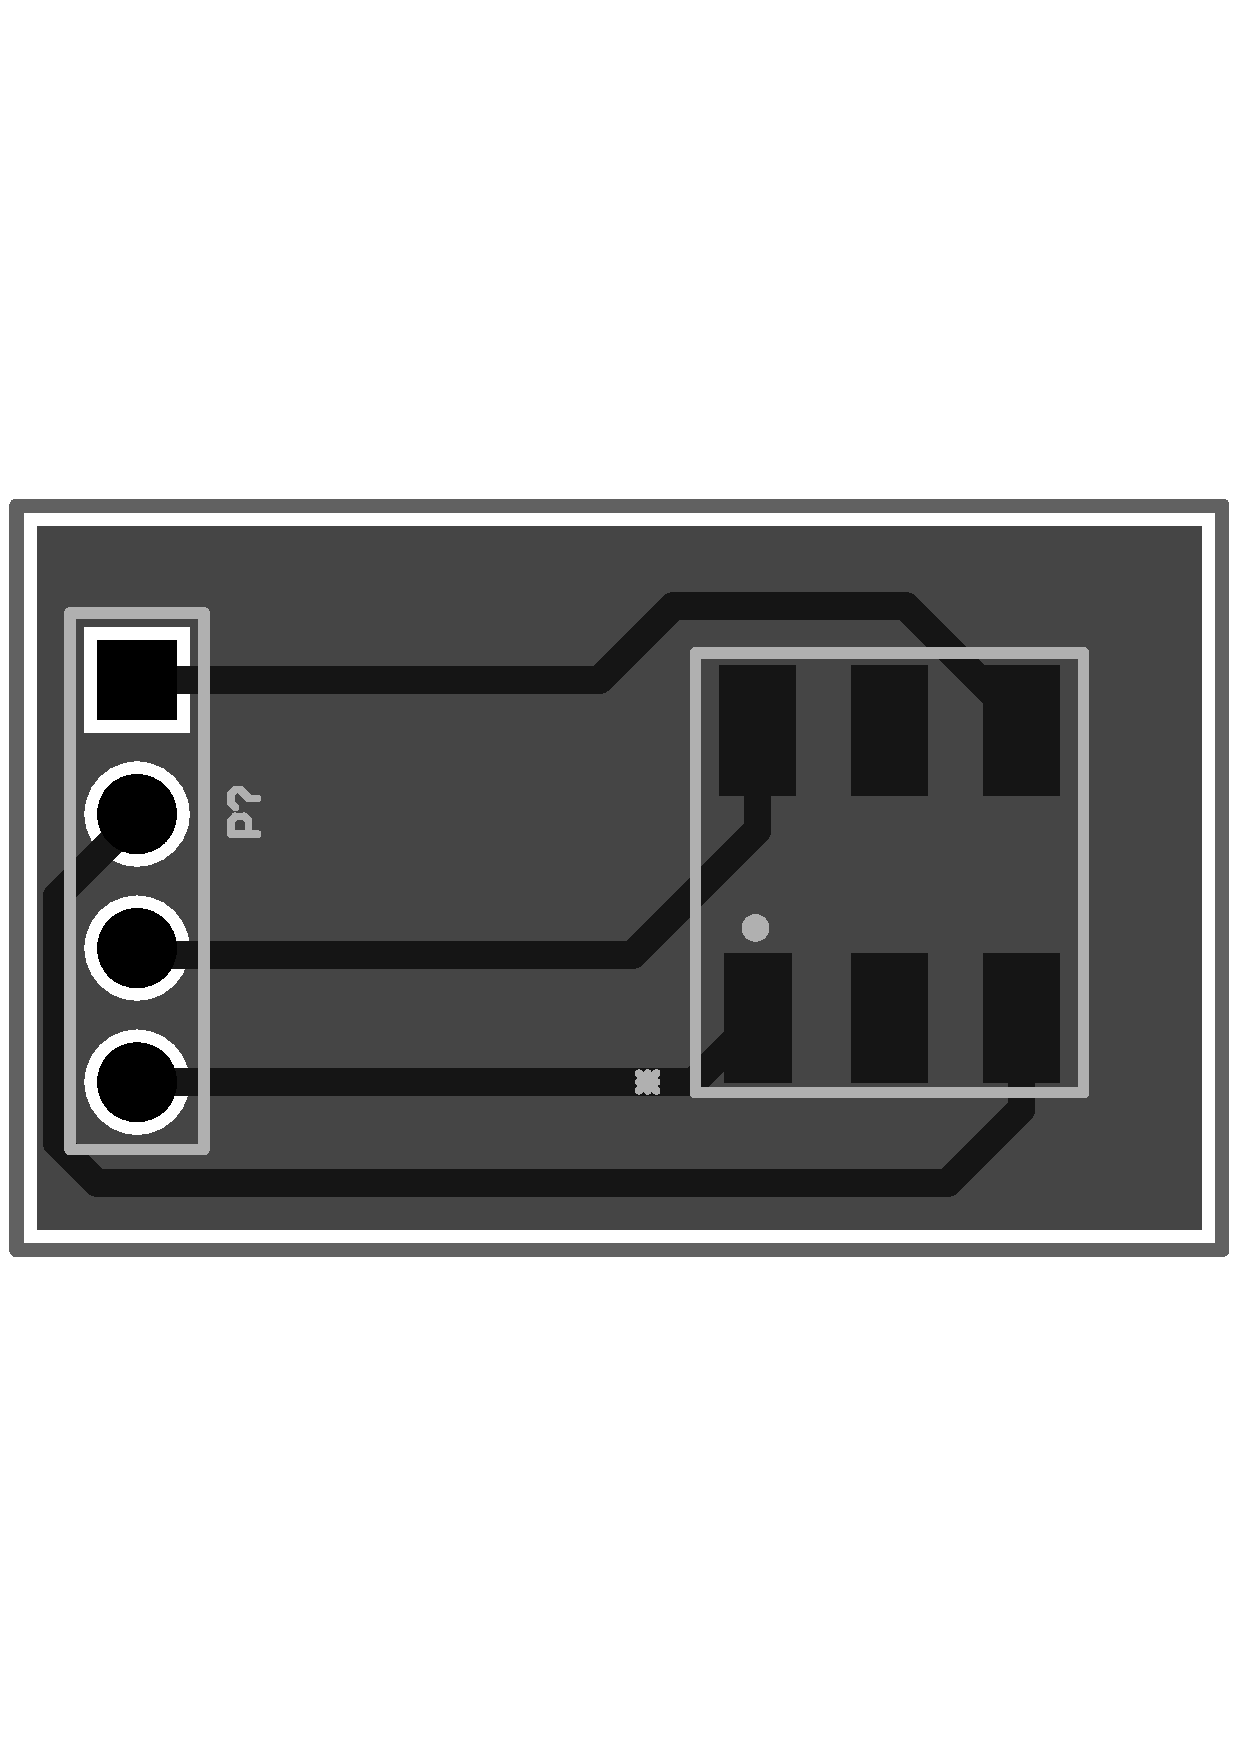
\includegraphics[angle=270, origin=c, clip, trim=0cm 0cm 0cm 0cm, width=1.00\textwidth]{PressureSensorPCB.pdf}
        \caption{Pressure Sensor PCB}
        \label{fig:pres_sense_pcb}
    \end{subfigure}
    \begin{subfigure}[t]{0.45 \textwidth}
        \centering
        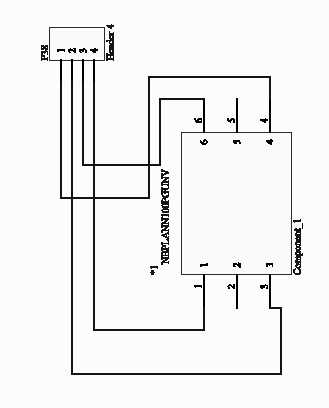
\includegraphics[angle=270, origin=c, clip, trim=0cm 0cm 0cm 0cm, width=1.00\textwidth]{PressureSensorSCH_crop.pdf}
        \caption{Pressure Sensor Schematic}
        \label{fig:pres_sense_sch}
    \end{subfigure}
    \caption{Pressure Sensor PCB}
    \label{fig:pres_sense}
\end{figure}

\subsubsection{Microcontroller}
\label{sub:microcontroller}

For an entire PNEUbot leg with 6 DoF, a minimum total of 12 muscles would be needed to achieve the required movement. This in turn would require 24 sensor inputs to read the pressure and position of each muscle. This requires a microcontroller that contains 24 ADC channels, one for each sensor, that can run fast enough to compute the control methods implemented and perform the sensor readings. The NUCLEO-STM32F722ZE \cite{nucleo_stm32f722ze} has 24 individual ADC channels available and runs with a maximum clock frequency of 216MHz, this microcontroller should allow enough processing overhead to achieve the required task.

\subsubsection{Electronics Shield}
\label{sub:shield}

In order to control the valves and read the pressure and potentiometer sensors a shield PCB, \Cref{fig:shield}, was designed to hold the logic level MOSFET control circuits for each valve. This board also contains a differential amplifier circuit, \Cref{sub:shieldshecmatic}, that is driven by the pressure sensor, with breakout headers for all the external sensors. The shield plugs into the microcontroller via the ST-Morpho connectors on the NUCLEO board.

\begin{figure}[!hbt]
    \begin{subfigure}[t]{0.45\textwidth}
        \centering
        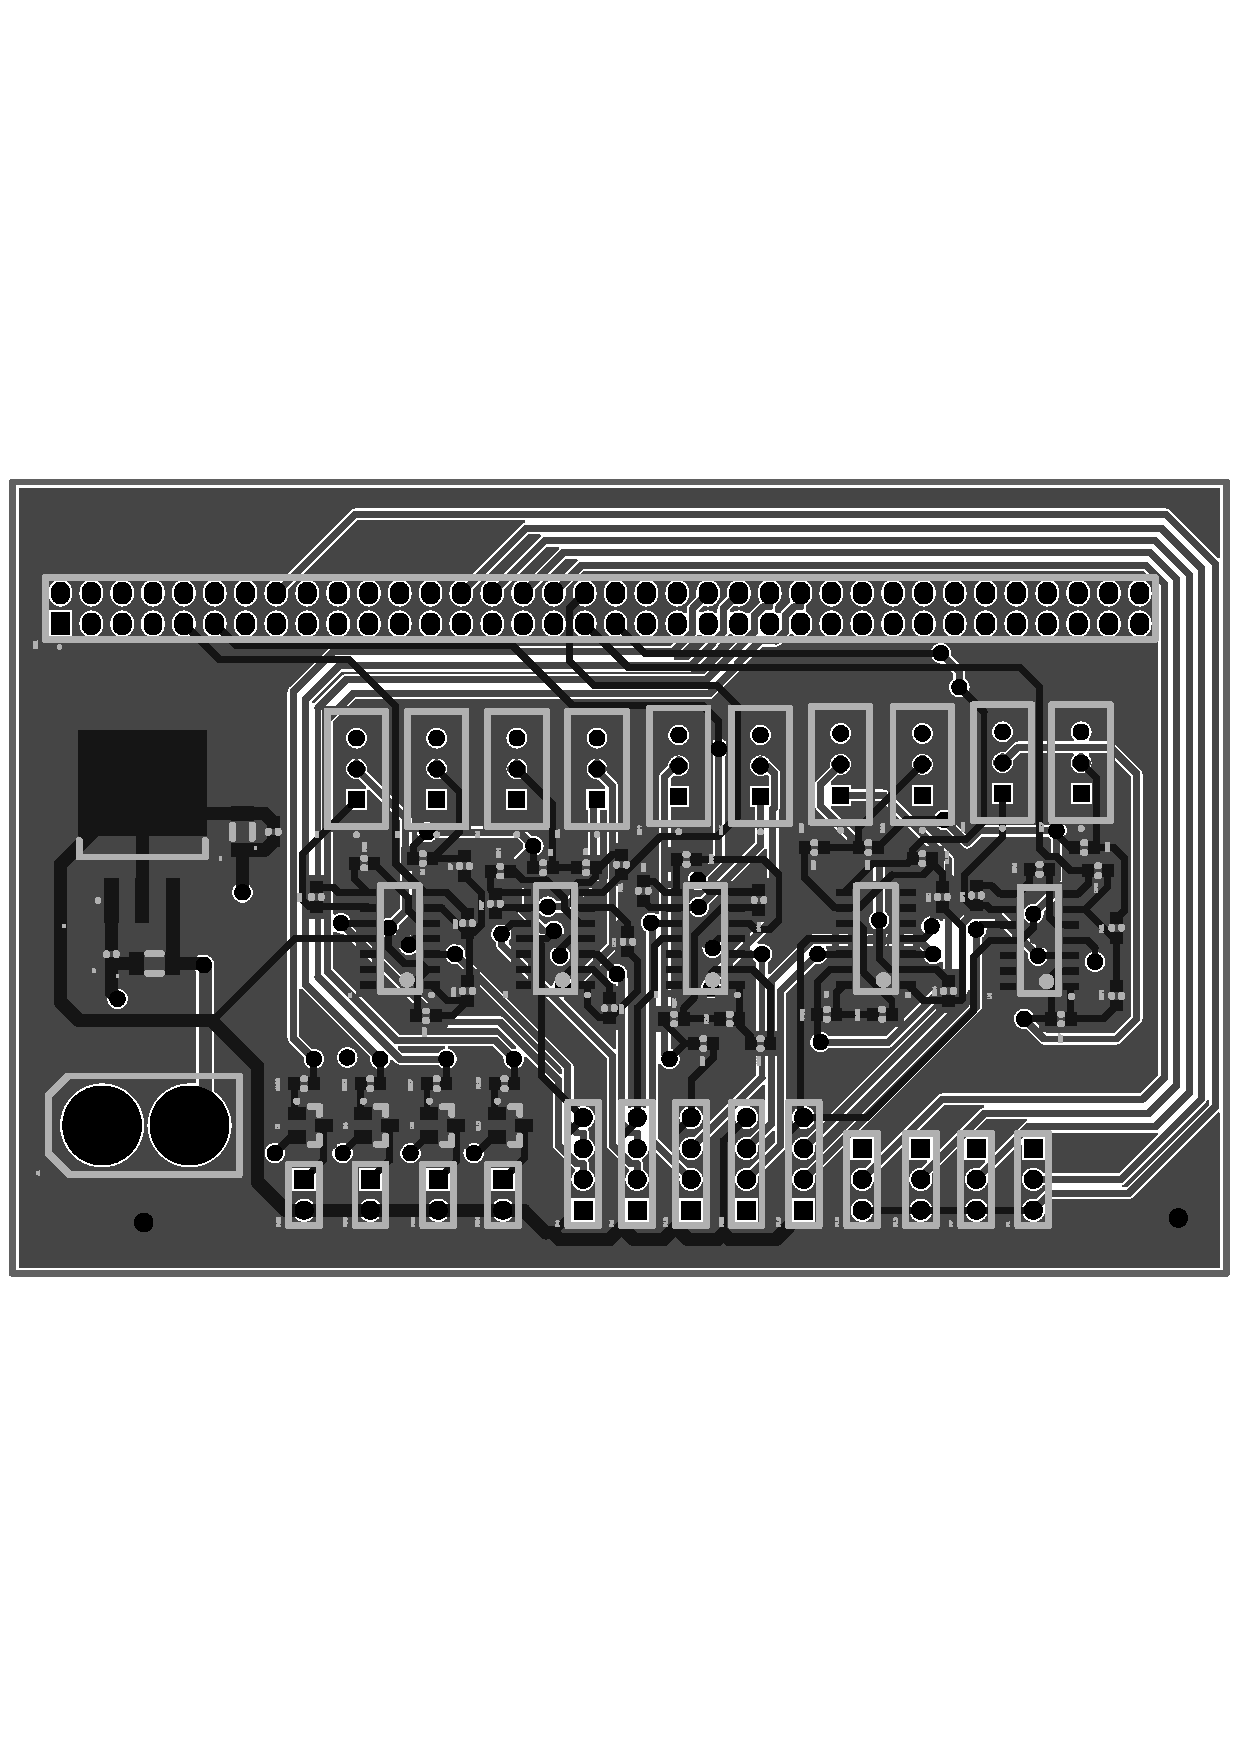
\includegraphics[angle=270, origin=c, clip, trim=0cm 8cm 0cm 8cm, width=1.00\textwidth]{ShieldPCB.pdf}
        \caption{Shield PCB}
        \label{fig:shield_PCB}
    \end{subfigure}
    \begin{subfigure}[t]{0.45\textwidth}
        \centering
        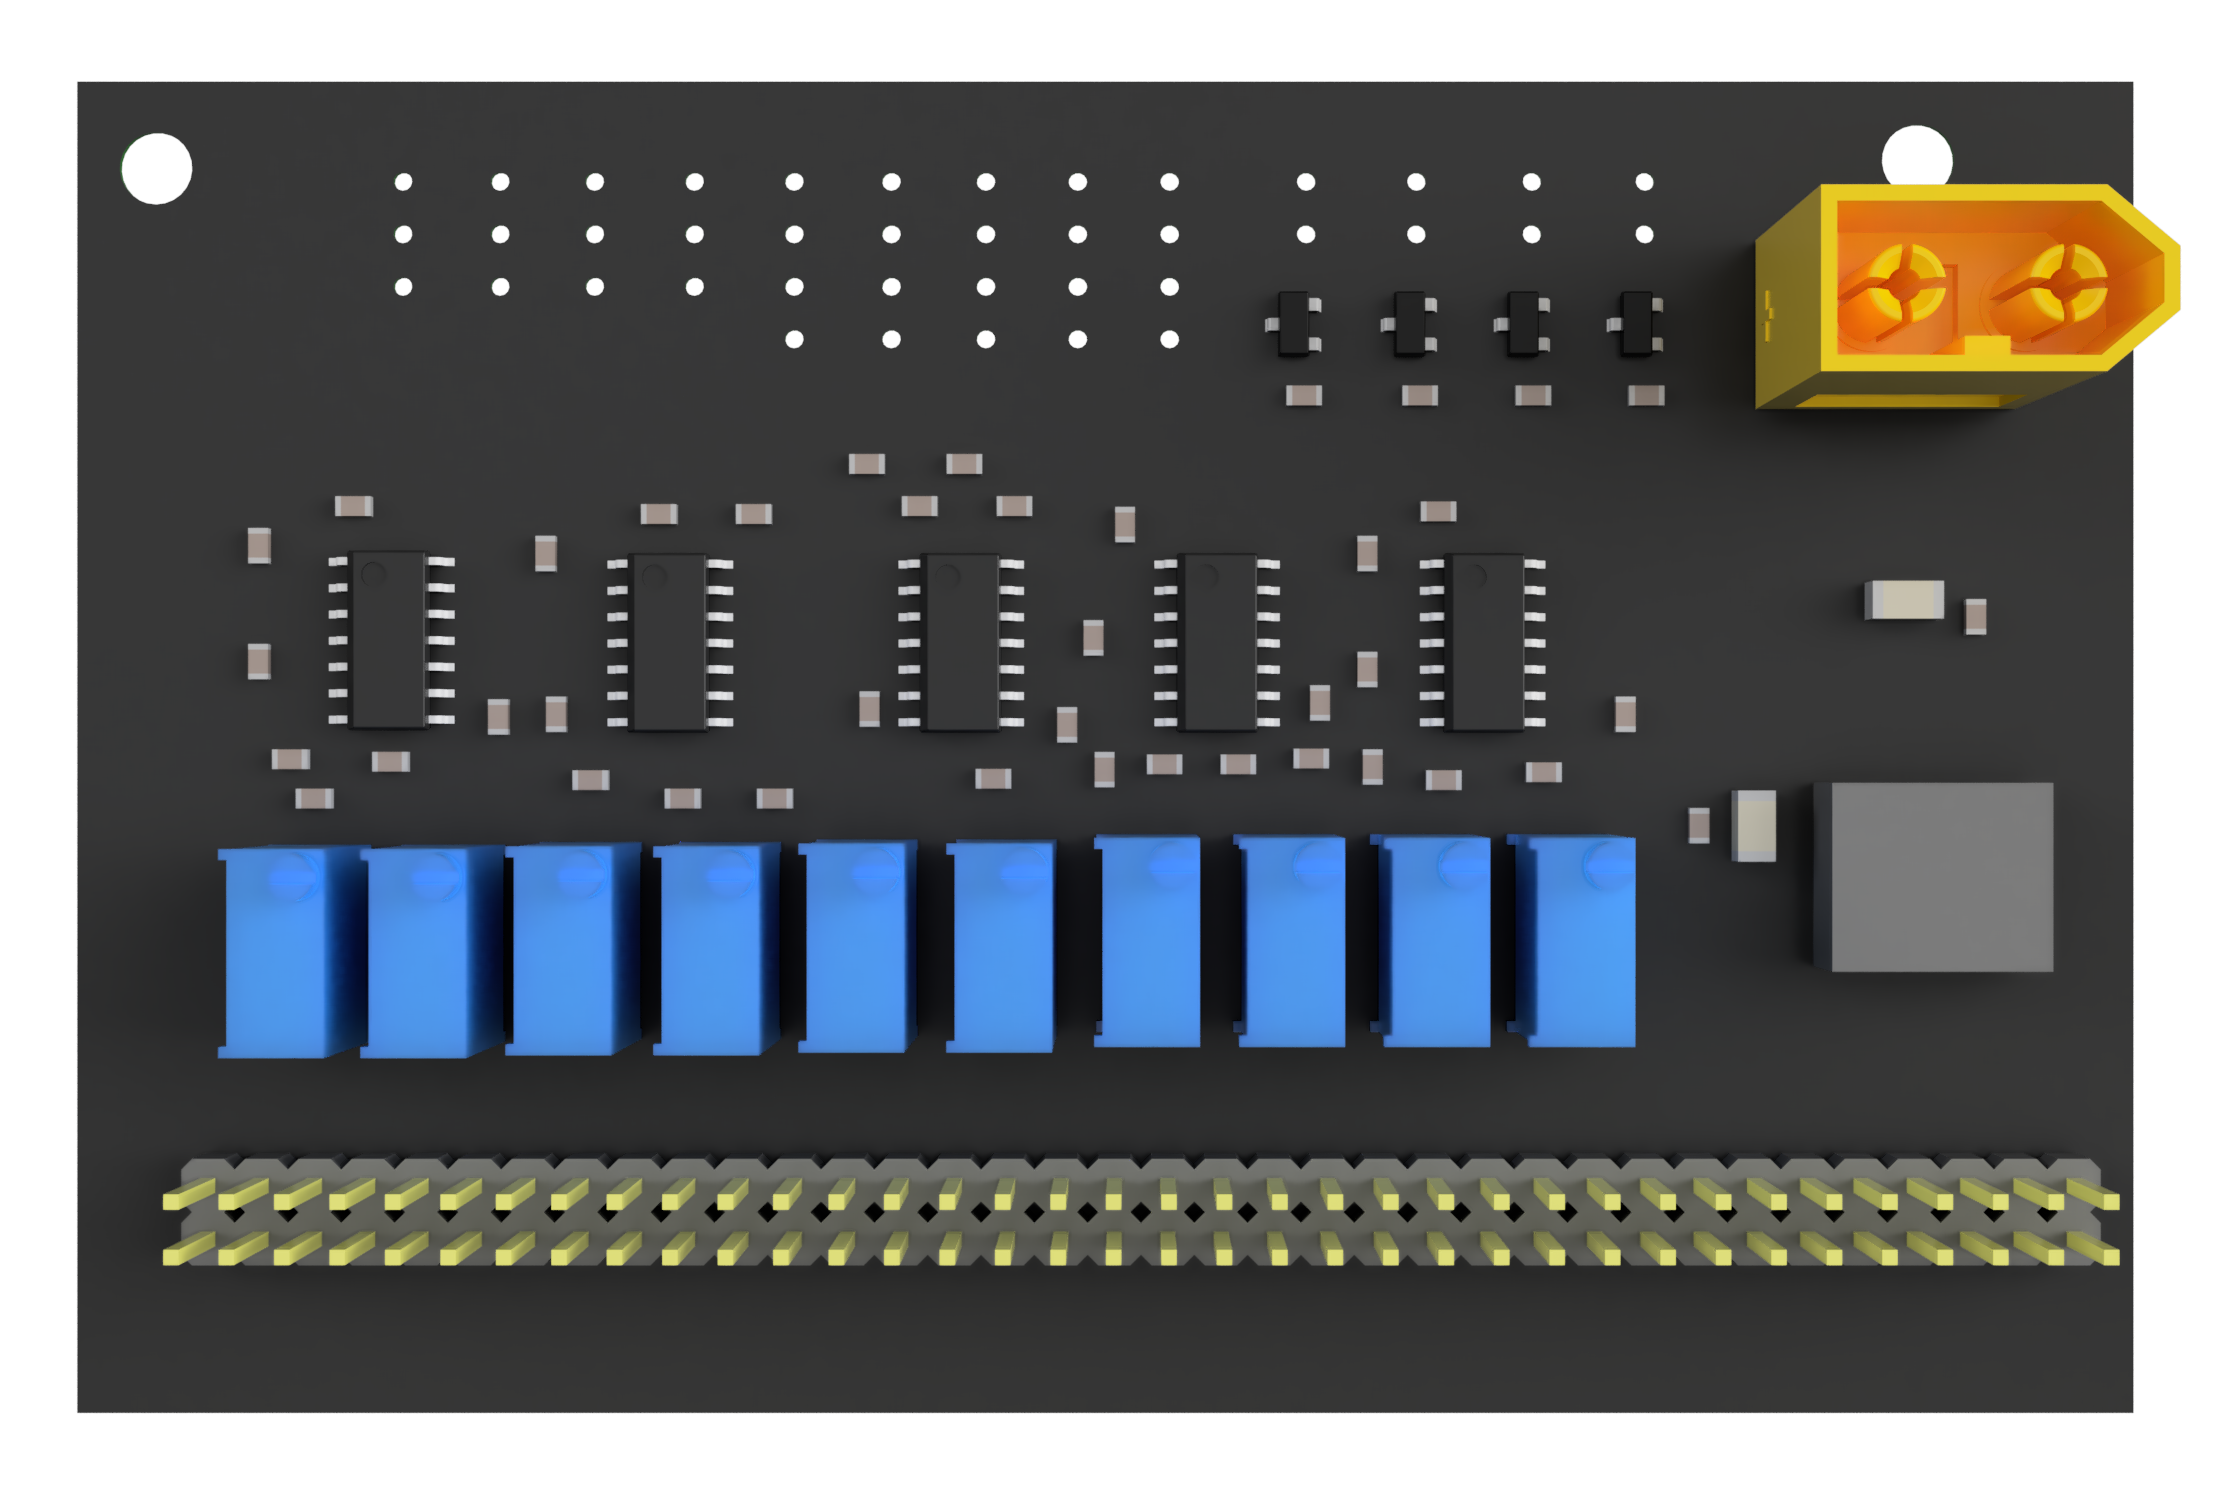
\includegraphics[angle=90, origin=c, clip, trim=1.5cm 0cm 1.5cm 0cm, width=1.00\textwidth]{Shield_Render.png}
        \caption{Shield Render}
        \label{fig:shield_render}
    \end{subfigure}
    \caption{Electronics Shield}
    \label{fig:shield}
\end{figure}

\clearpage
\section{Modelling and Control}
\label{section:modeling_and_control}

\subsection{Muscle Modelling}
\label{sub:muscle_modelling}
As this project is focused on the development of a framework and single degree of freedom pneumatic joint the model used has been taken from an existing source \cite{hosovsky_2012}. As mentioned in \Cref{sub:dynamic_modelling} the modelling of a pneumatic muscle can be approached as a mechanically derived nonlinear mass spring damper \Cref{fig:massspringdamper}. The stiffness of the spring can be controlled as a function of the muscle pressure. This relationship can be approximated by a fifth order polynomial of two variables of twenty-one coefficients. The pneumatic part of the model is divided into two main components, the model of volume flow rate through the valves and a differential equation for the muscle pressure. The use of on/off style solenoid valves simplifies the flow rate to either a constant compressor pressure or atmospheric pressure, solely dependent on the muscle pressure. The second pneumatic component is the derivative time dependent equation derived from ideal gas laws. Below is the equation found representing these forces \Cref{math:dynamicforce2}, where m - moving mass (kg), y - muscle displacement (m), F\textsubscript{S}(k,P\textsubscript{m}) - nonlinear term representing a variable spring force (N), F\textsubscript{D}(\.{k},P\textsubscript{m}) - nonlinear term representing a variable damper force (N), F\textsubscript{E} - external force (N), k - muscle contraction (defined as k = k\textsubscript{0} + y/l\textsubscript{0} where k\textsubscript{0} is the initial contraction and l\textsubscript{0} is the initial muscle length (-) and P\textsubscript{m} - the absolute muscle pressure (Pa). The full equation can be found in \Cref{sub:dynamicforcederive}.

\begin{equation}
    \ddot{y} = \frac{1}{m}[F_E-F_S(k,P_m)-F_D(\dot{k},P_m)]
    \label{math:dynamicforce2}
\end{equation}

\begin{figure}[hbt!]
    \centering
    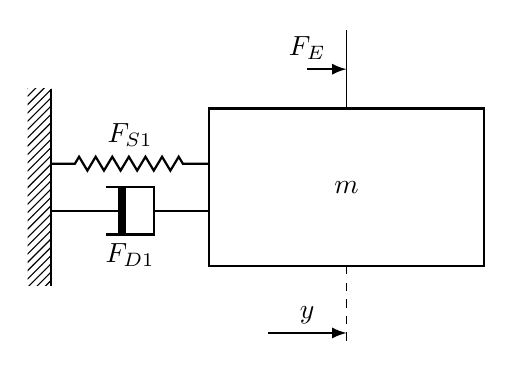
\begin{tikzpicture}[every node/.style={outer sep=0pt},thick,
        mass/.style={draw,thick},
        spring/.style={thick,decorate,decoration={zigzag,pre length=0.3cm,post
        length=0.3cm,segment length=6}},
        ground/.style={fill,pattern=north east lines,draw=none,minimum
        width=0.75cm,minimum height=0.3cm},
        dampic/.pic={\fill[white] (-0.1,-0.3) rectangle (0.3,0.3);
        \draw (-0.3,0.3) -| (0.3,-0.3) -- (-0.3,-0.3);
        \draw[line width=1mm] (-0.1,-0.3) -- (-0.1,0.3);}]
        
          % Mass
        \node[mass,minimum width=3.5cm,minimum height=2cm] (m1) {$m$};
        % Left Wall
        \node[left=2cm of m1,ground,minimum width=3mm,minimum height=2.5cm] (g1){};
        \draw (g1.north east) -- (g1.south east);
        
        \draw[spring] ([yshift=3mm]g1.east) coordinate(aux) -- (m1.west|-aux) node[midway,above=1mm]{$F_{S1}$};
        
        \draw ([yshift=-3mm]g1.east) coordinate(aux') -- (m1.west|-aux') pic[midway]{dampic} node[midway,below=3mm]{$F_{D1}$};
        
        \draw[thin] (m1.north) -- ++ (0,1) coordinate[midway](aux1);
        \draw[latex-] (aux1) -- ++ (-0.5,0) node[above]{$F_E$}; 
        \draw[thin,dashed] (m1.south) -- ++ (0,-1) coordinate[pos=0.85](aux'1);
        \draw[latex-] (aux'1) -- ++ (-1,0) node[midway,above]{$y$};

    \end{tikzpicture}
    \caption{Mass Spring Damper}
    \label{fig:massspringdamper}
\end{figure}

However, this system only describes the dynamics of a single muscle arrangement, which is not the arrangement used in the project. To derive an equation that represents the dynamics of a two muscle system a few assumptions can be made. 
\begin{itemize}
  \item The position and by inheritance the velocity of a only single muscle is required to be known to solve the differential equations. This is due to the rigid nature of the coupling between the two muscles. 
  \item The friction lost at the pivot point is negligible.
  \item The nylon line that attaches the two muscles cannot stretch and remains taught at all times.
  \item The mass of the two muscles is combined into a single mass.
\end{itemize}

From these assumptions the model \Cref{math:dynamicforce2} above can be altered to the form the following \Cref{math:two_muscle_ode}. This is analogous to a double mass spring damper with two fixed ends, \Cref{fig:doublemassspringdamper}:

\begin{equation}
    \ddot{y} = \frac{1}{m}[F_E-F_{S2}(k_2,P_{m2})-F_{S1}(k_1,P_{m1})-F_{D2}(\dot{k_2},P_{m2})-F_{D1}(\dot{k_1},P_{m1})]
    \label{math:two_muscle_ode}
\end{equation}

\begin{figure}[hbt!]
    \centering
    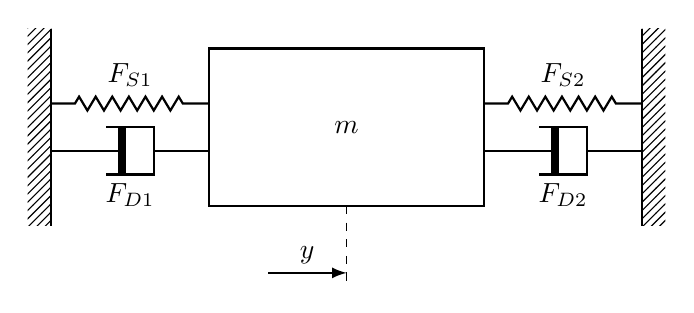
\begin{tikzpicture}[every node/.style={outer sep=0pt},thick,
        mass/.style={draw,thick},
        spring/.style={thick,decorate,decoration={zigzag,pre length=0.3cm,post
        length=0.3cm,segment length=6}},
        ground/.style={fill,pattern=north east lines,draw=none,minimum
        width=0.75cm,minimum height=0.3cm},
        dampic/.pic={\fill[white] (-0.1,-0.3) rectangle (0.3,0.3);
        \draw (-0.3,0.3) -| (0.3,-0.3) -- (-0.3,-0.3);
        \draw[line width=1mm] (-0.1,-0.3) -- (-0.1,0.3);}]
        
          % Mass
        \node[mass,minimum width=3.5cm,minimum height=2cm] (m1) {$m$};
        % Left Wall
        \node[left=2cm of m1,ground,minimum width=3mm,minimum height=2.5cm] (g1){};
        \draw (g1.north east) -- (g1.south east);
        % Right Wall
        \node[right=2cm of m1,ground,minimum width=3mm,minimum height=2.5cm] (g2){};
        \draw (g2.north west) -- (g2.south west);
        
        \draw[spring] ([yshift=3mm]g1.east) coordinate(aux) -- (m1.west|-aux) node[midway,above=1mm]{$F_{S1}$};
        \draw[spring]  (m1.east|-aux) -- (g2.west|-aux) node[midway,above=1mm]{$F_{S2}$};
        
        \draw ([yshift=-3mm]g1.east) coordinate(aux') -- (m1.west|-aux') pic[midway]{dampic} node[midway,below=3mm]{$F_{D1}$}
         (m1.east|-aux') -- (g2.west|-aux') pic[midway]{dampic} node[midway,below=3mm]{$F_{D2}$};
        
        \draw[thin,dashed] (m1.south) -- ++ (0,-1) coordinate[pos=0.85](aux'1);
        \draw[latex-] (aux'1) -- ++ (-1,0) node[midway,above]{$y$};

    \end{tikzpicture}
    \caption{Mass Spring Damper Pair}
    \label{fig:doublemassspringdamper}
\end{figure}

To make calculating the system equations more manageable a state space representation \Cref{math:state_space_representation} of the second order ODE can be calculated using the states in \Cref{math:state_space_matrix}, resulting in the following set of equations. These equations don't strictly contain any input or output variables and thus reduce to only a single $\boldsymbol{A}$ matrix. All symbols present in the $\boldsymbol{A}$ matrix are taken directly from \Cref{math:dynamicforce2} and are then modified to represent the first or second muscles. A complete list of symbols can be found in \Cref{sub:Amatderive}.\newline

\begin{align}
    \label{math:state_space_representation}
    \dot{x} &= \boldsymbol{A}x + \boldsymbol{B}u\\
    y &= \boldsymbol{C}x + \boldsymbol{D}u\nonumber 
\end{align}

\begin{equation}
\begin{bmatrix}
        \dot{y}\\
        \ddot{y}\\
        \dot{P_{m1}}\\
        \dot{P_{m2}}\\
    \end{bmatrix}
    = \fdv{F}{z}\left[\boldsymbol{\chi}\right]
    \begin{bmatrix}
        y\\
        \dot{y}\\
        P_{m1}\\
        P_{m2}\\
    \end{bmatrix}
    \label{math:state_space_matrix}
\end{equation}
where
\begin{equation*}
        \boldsymbol{\chi} = 
    \begin{bmatrix}
        \dot{y}\\
        \frac{1}{m}[-F_{S2}(k_2,P_{m2})-F_{S1}(k_1,P_{m1})-F_{D2}(\dot{k_2},P_{m2})-F_{D1}(\dot{k_1},P_{m1})]\\
        \frac{1}{V_{m1}}(P_a\dot{V_{a1}}-P_{m1}\dot{V_{m1}})\\
        \frac{1}{V_{m2}}(P_a\dot{V_{a2}}-P_{m2}\dot{V_{m2}})\\
    \end{bmatrix}
\end{equation*}

The partial differential of each state function with respect to each state then forms the final $\boldsymbol{A}$ matrix \Cref{math:A_matrix}. Converting this system into a discrete time representation can then be done using Eulers Approximation \Cref{math:discrete_formula}, resulting in the \Cref{math:discretistion_model} which is then used as the state update calculation. \newline

\begin{equation}
    \boldsymbol{A} =
    \begin{bmatrix}
        0 & 1 & 0 & 0\\
        \alpha_{10} & \alpha_{11} & \alpha_{12} & \alpha_{13}\\
        \alpha_{20} & \alpha_{21} & \alpha_{22} & 0\\
        \alpha_{30} & \alpha_{31} & 0 & \alpha_{33}\\
    \end{bmatrix}
    \label{math:A_matrix}
\end{equation}

\begin{equation}
        x\left[\boldsymbol{k+1}\right] = \left(\boldsymbol{\boldsymbol{I}+T_s\boldsymbol{A}}\right)x\left[\boldsymbol{k}\right]
    \label{math:discrete_formula}
\end{equation}

\begin{equation}
    \begin{bmatrix}
        y\left[\boldsymbol{k+1}\right]\\
        \dot{y}\left[\boldsymbol{k+1}\right]\\
        P_{m1}\left[\boldsymbol{k+1}\right]\\
        P_{m2}\left[\boldsymbol{k+1}\right]\\
    \end{bmatrix}
    =
    \left(
    \begin{bmatrix}
        1 & 0 & 0 & 0\\
        0 & 1 & 0 & 0\\
        0 & 0 & 1 & 0\\
        0 & 0 & 0 & 1\\
    \end{bmatrix}
    + T_s
    \begin{bmatrix}
        0 & 1 & 0 & 0\\
        \alpha_{10} & \alpha_{11} & \alpha_{12} & \alpha_{13}\\
        \alpha_{20} & \alpha_{21} & \alpha_{22} & 0\\
        \alpha_{30} & \alpha_{31} & 0 & \alpha_{33}\\
    \end{bmatrix}
    \right)
    \begin{bmatrix}
        y\left[\boldsymbol{k}\right]\\
        \dot{y}\left[\boldsymbol{k}\right]\\
        P_{m1}\left[\boldsymbol{k}\right]\\
        P_{m2}\left[\boldsymbol{k}\right]\\
    \end{bmatrix}
    \label{math:discretistion_model}
\end{equation}\newline

To complete the model of the pneumatic muscles the remaining constant variables must be known, some of these are taken from the model paper \cite{hosovsky_2012}, and some are muscle dependent parameters, the most complex of which is an approximation of the force produced by the muscle to the pressure and contraction length in a 21 coefficient polynomial.

\subsubsection{Static Mapping}
\label{sub:static_mapping}
The static map represents the relationship of force produced by the muscle to the pressure and contraction length. This can be approximated by a fifth order polynomial of two variables of representing a 21 coefficient polynomial, reduced into an upper left hand triangle 6x6 matrix surrounded by two vector multiplications \Cref{math:fce_matrix}. This surface has been calculated in Matlab using the model from \cite{martens_boblan_2017} as the relationship between the three variables, \Cref{fig:staticmap}. From this surface a polynomial can be fit approximated as a 5\textsuperscript{th} order polynomial. As seen in the table below \Cref{tab:polynomial_coefficients} the coefficients calculated are within 95\% of the surface.

\begin{equation}
F_{S}(k,P_m) = 
\begin{bmatrix}
        1 & k & k^2 & k^3 & k^4 & k^5\\
    \end{bmatrix}
    \begin{bmatrix}
        \rho_{00} & \rho_{01} & \rho_{02} & \rho_{03} & \rho_{04} & \rho_{05}\\
        \rho_{10} & \rho_{11} & \rho_{12} & \rho_{13} & \rho_{14} & 0\\
        \rho_{20} & \rho_{21} & \rho_{22} & \rho_{23} & 0         & 0\\
        \rho_{30} & \rho_{31} & \rho_{32} & 0         & 0         & 0\\
        \rho_{40} & \rho_{41} & 0         & 0         & 0         & 0\\
        \rho_{50} & 0         & 0         & 0         & 0         & 0\\
    \end{bmatrix}
    \begin{bmatrix}
        1\\
        P_m\\
        P_m^2\\
        P_m^3\\
        P_m^4\\
        P_m^5\\
    \end{bmatrix}
    \label{math:fce_matrix}
\end{equation}
\begin{table}[!hbt]
    \centering
    \caption{Polynomial Coefficients}
    \begin{tabular}{|r||r|r|r|}
        \hline
            \multicolumn{4}{|c|}{Polynomial Coefficients} \\
        \hline
            Matrix Element & Mean Coefficient & Minimum & Maximum\\
        \hline
            $\rho_{00}$ & $76.27$      & $76.25$      & $76.29$\\
            $\rho_{10}$ & $1.515e+12$  & $-1.512e+13$ & $1.815e+13$\\
            $\rho_{01}$ & $-1.515e+12$ & $-1.815e+13$ & $1.512e+13$\\
            $\rho_{20}$ & $7.645e+12$  & $-3.98e+12$  & $1.927e+13$\\
            $\rho_{11}$ & $-1.984e+13$ & $-3.816e+13$ & $-1.518e+12$\\
            $\rho_{02}$ & $1.219e+13$  & $-2.637e+12$ & $2.702e+13$\\
            $\rho_{30}$ & $-1.535e+13$ & $-3.118e+13$ & $4.877e+11$\\
            $\rho_{21}$ & $3.063e+13$  & $9.519e+12$  & $5.174e+13$\\
            $\rho_{12}$ & $-1.087e+13$ & $-3.451e+13$ & $1.277e+13$\\
            $\rho_{03}$ & $-4.412e+12$ & $-2.166e+13$ & $1.284e+13$\\
            $\rho_{40}$ & $2.531e+13$  & $1.529e+13$  & $3.532e+13$\\
            $\rho_{31}$ & $-2.712e+13$ & $-3.913e+13$ & $-1.511e+13$\\
            $\rho_{22}$ & $-1.771e+13$ & $-2.676e+13$ & $-8.651e+12$\\
            $\rho_{13}$ & $1.455e+13$  & $9.587e+11$  & $2.814e+13$\\
            $\rho_{04}$ & $4.974e+12$  & $-5.777e+12$ & $1.572e+13$\\
            $\rho_{50}$ & $-1.836e+12$ & $-4.701e+12$ & $1.03e+12$\\
            $\rho_{41}$ & $3.682e+12$  & $1.3e+12$    & $6.063e+12$\\
            $\rho_{32}$ & $2.06e+12$   & $-9.788e+11$ & $5.098e+12$\\
            $\rho_{23}$ & $-6.712e+12$ & $-9.919e+12$ & $-3.506e+12$\\
            $\rho_{14}$ & $1.642e+12$  & $-9.098e+11$ & $4.195e+12$\\
            $\rho_{05}$ & $1.164e+12$  & $-1.678e+12$ & $4.006e+12$\\
        \hline
    \end{tabular}
    \label{tab:polynomial_coefficients}
\end{table}

To verify the accuracy of the calculated static map, an experiment was conducted by varying the pressure and mass attached to a static muscle. Varying the pressure from 0 to 60 psi, and mass from 1.5 to 16 kg. From this the length of the muscle can be measured and a static response plot formed. \Cref{fig:static_response_ideal} shows the ideal static response curve of the pneumatic muscles.
\Cref{fig:static_response_latex} shows the experimental static responses for varying masses for a muscle with a latex bladder. \Cref{fig:static_response_bike} shows the experimental static responses for varying masses for a muscle with a bike tube bladder. \newline 
The ideal model does not fit the experimental results closely. For the latex bladder the experimental data contains inaccuracy in the measurement of the pressure within the muscle. This is seen in the overlapping force curves of the plot. The model does not capture the behaviour at low pressures. The bike tube bladder the results closer represent the ideal model. Again, the model does not capture the behaviour at low pressures. For this experiment an artefact can be seen in the 0 to 10 psi range of the 1.5 kg test. This artefact is a result of the muscle extending prior to contracting under the pressure. The minimum weight required to fully extend the muscle under 0 psi was not achieved.

\begin{figure}[!hbt]
    \centering
    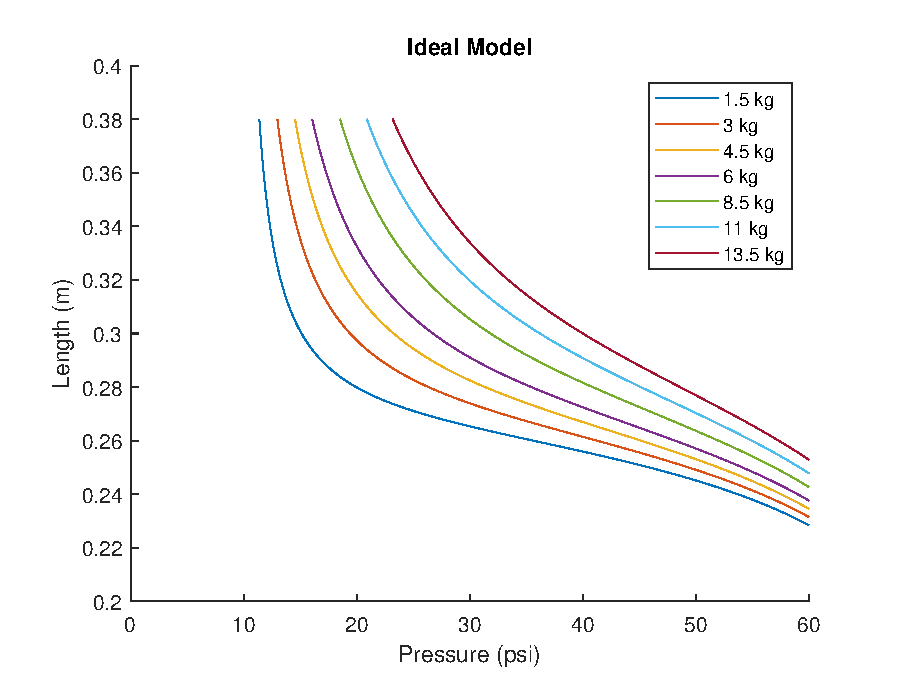
\includegraphics[scale=0.8]{IdealModel.eps}
    \caption{Ideal Static Response}
    \label{fig:static_response_ideal}
\end{figure}

\begin{figure}[!hbt]
    \centering
    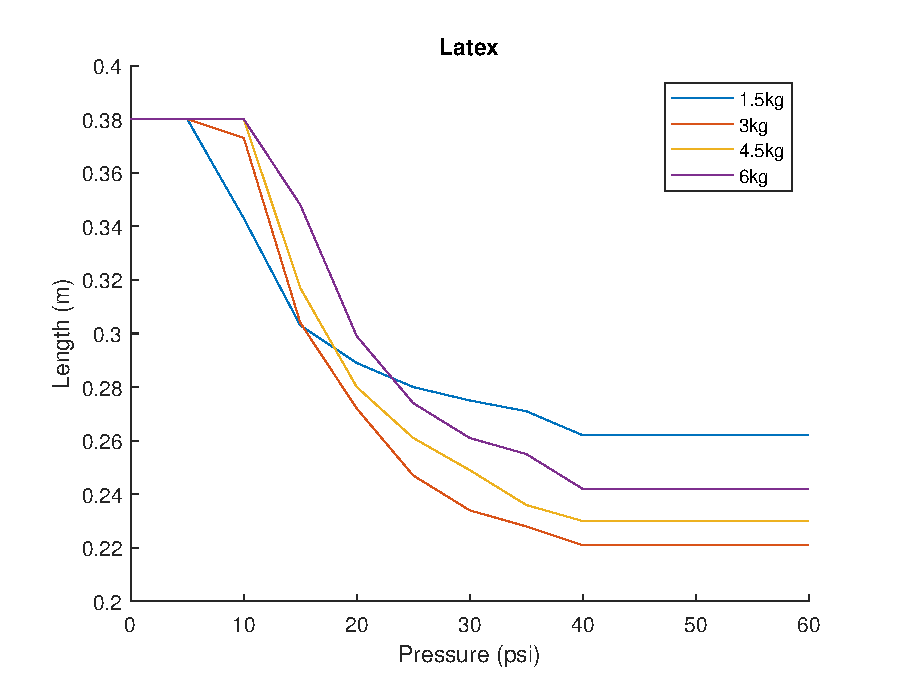
\includegraphics[scale=0.8]{latex.eps}
    \caption{Static Response Latex Bladder}
    \label{fig:static_response_latex}
\end{figure}

\begin{figure}[!hbt]
    \centering
    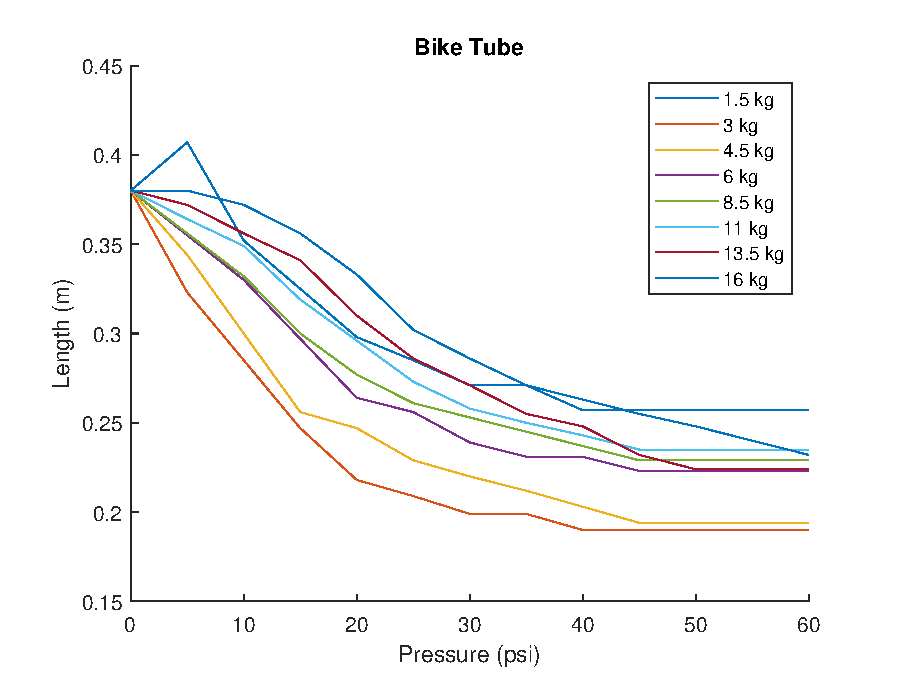
\includegraphics[scale=0.8]{BikeTube.eps}
    \caption{Static Response Bike Tube Bladder}
    \label{fig:static_response_bike}
\end{figure}

\subsection{Control System}
\label{sub:control_system}
In order to achieve robust control over the nonlinear actuators an implementation of model predictive control (MPC) was chosen to provide the control structure for the system, the outline of which can be seen in \Cref{fig:control_diagram_overview}. This controller will be compared in simulation to implementations of other available controllers, a PID and SMC.The MPC control structure utilises a preview (prediction) horizon to estimate the future trajectory of the system based on the current state and a series of inputs to the system. This prediction horizon is calculated to 'p' time in the future, only requiring past knowledge of the system status. However, to achieve this an estimation of the system response to any arbitrary system state and input is required to calculate the trajectory. Since the model of the pneumatic muscles is highly nonlinear, there are four main options for solving future estimations.
\begin{itemize}
    \item Solve the nonlinear ODE using brute force or recursion
    \item Offline linearisation about a single operating point
    \item Offline linearisation about multiple operating points stored in a lookup table
    \item Online linearisation about the current operating point
\end{itemize}

The first solution to solve the nonlinear ODE involves a large computational overhead and may not be possible in real-time, however this solution would result in the best estimation of the next system state. The second and third options are less computationally intense and would guarantee a real-time solution however are both less accurate due to the finite number of linearised solutions stored and in the case of the third option can be memory heavy. The final of these solutions, and the one chosen for this project requires calculating the linearisation of the system at each sample time. This whilst being somewhat computationally expensive is minor compared to the first method, and requires little memory, whilst reducing the error between the linearised operating point and the nonlinear system.\newline

\begin{figure}[!hbt]
    \centering
    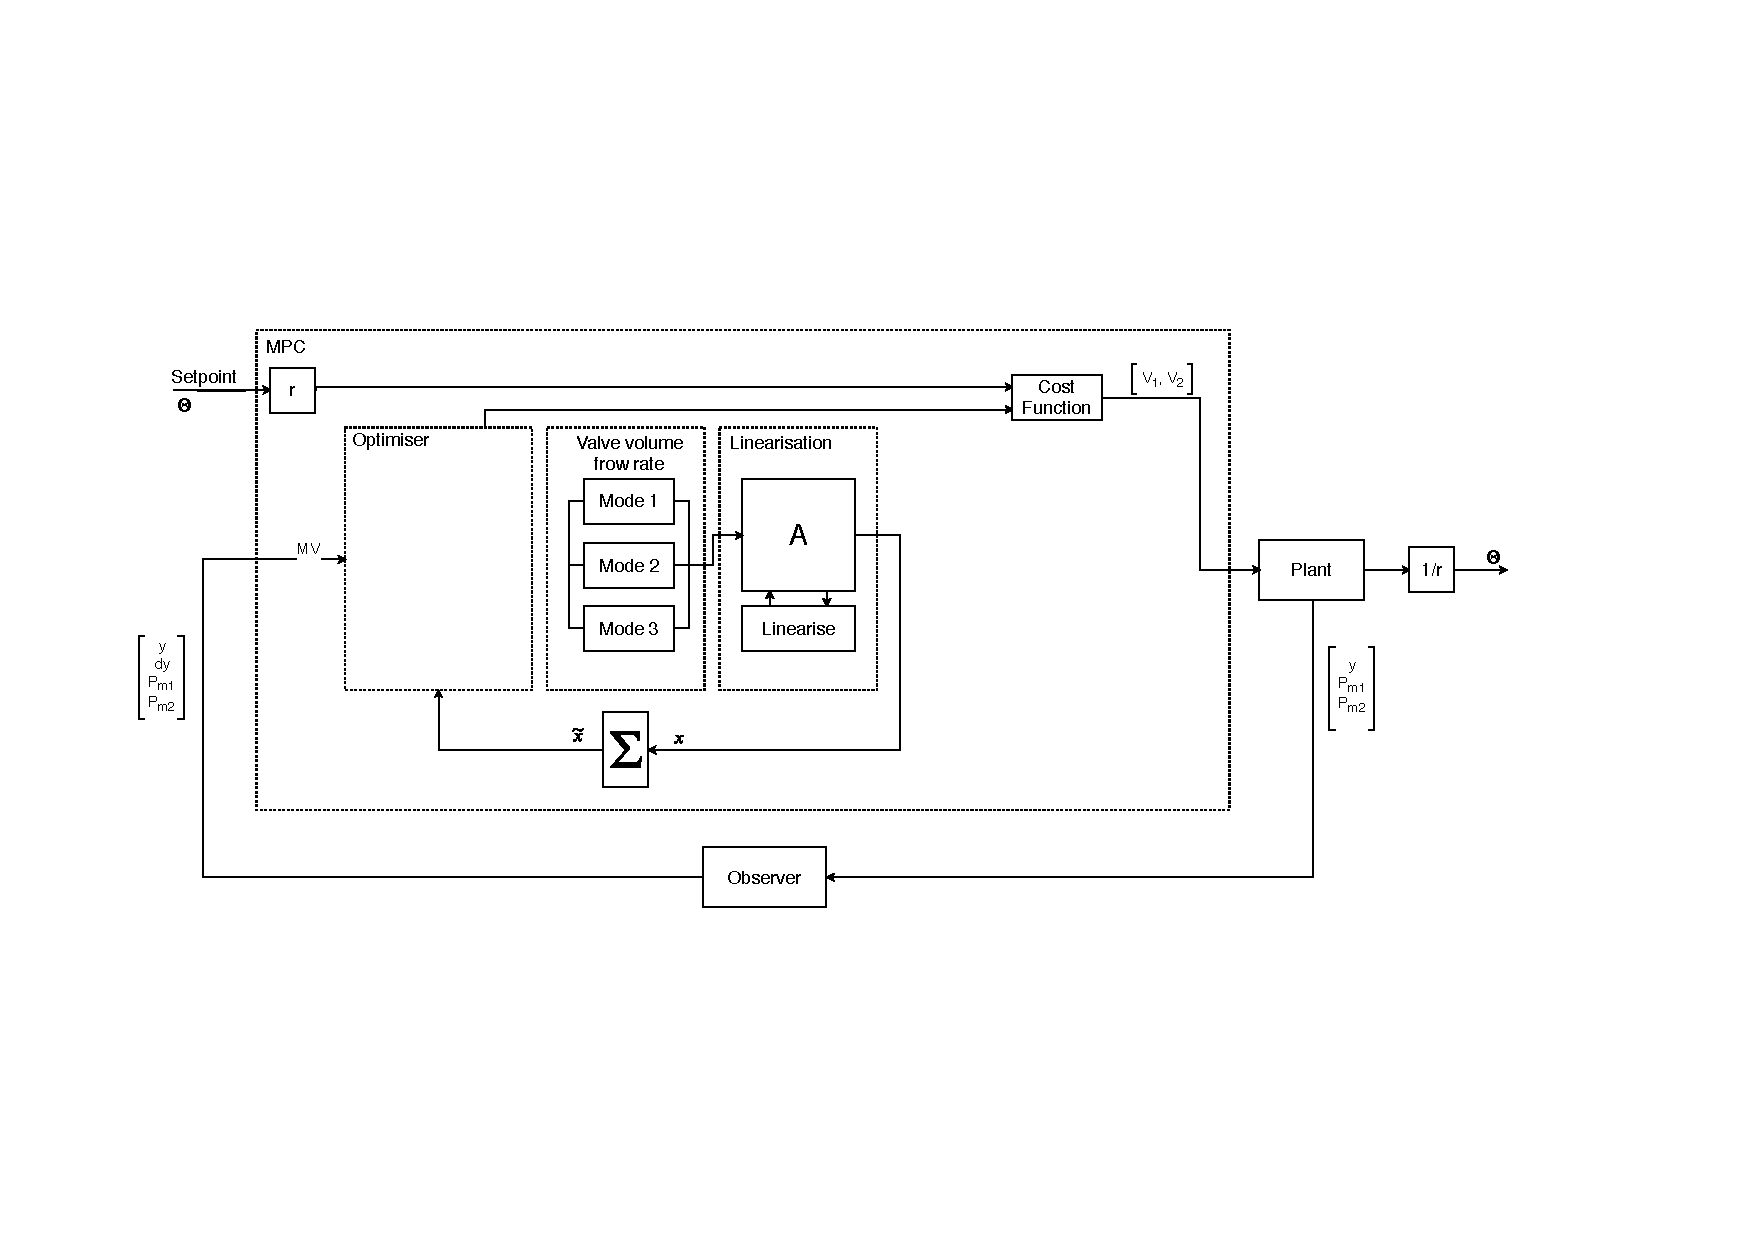
\includegraphics[clip, trim=2cm 4cm 4cm 4cm, width=1.00\textwidth]{BlockDiagram_Overview.pdf}
    \caption{Control Diagram}
    \label{fig:control_diagram_overview}
\end{figure}

As the goal of MPC is to calculate a series of predicted control inputs that reduce the error between the reference trajectory and predicted/measured output, a method of selecting a set of control inputs is required that will give rise to a new estimation. As mentioned in \Cref{subsubsection:pneumatic_control} and \Cref{tab:valve_states} the system implemented has a limited number of control actions that can be performed to produce an output. As this is the case all three modes will be used to subsequently calculate differing estimations for the predicted control input. \newline

A method for calculating the predicted output trajectory given a set of predicted control inputs, is with the use of a preview horizon controller or optimiser. The optimiser calculates the updated states for each control input recursively solving this for some 'p' layers of future control input, this design is highlighted in \Cref{fig:control_diagram_optimiser}. As there are three inputs considered for each seed the problem has 3\textsuperscript{p} complexity growing rapidly with the increase in the prediction horizon. The function of the optimiser is to calculate the 'cost' \Cref{math:cost_function} or weighted error of performing the root seed control action to some desired setpoint and states with respect to the final inputs and states. This is calculated on the completion of each final seed within the optimiser, the cost is then sorted to determine the optimal initial control action to perform. A linear quadratic cost function is used due to the linear constraints of the system.

\begin{equation}
    J = \sum_{k=0}^{T_s} x\left[k\right]^T\textbf{Q}x\left[k\right] + u\left[k\right]^T\textbf{R}u\left[k\right]
    \label{math:cost_function}
\end{equation}

\begin{figure}[!hbt]
    \centering
    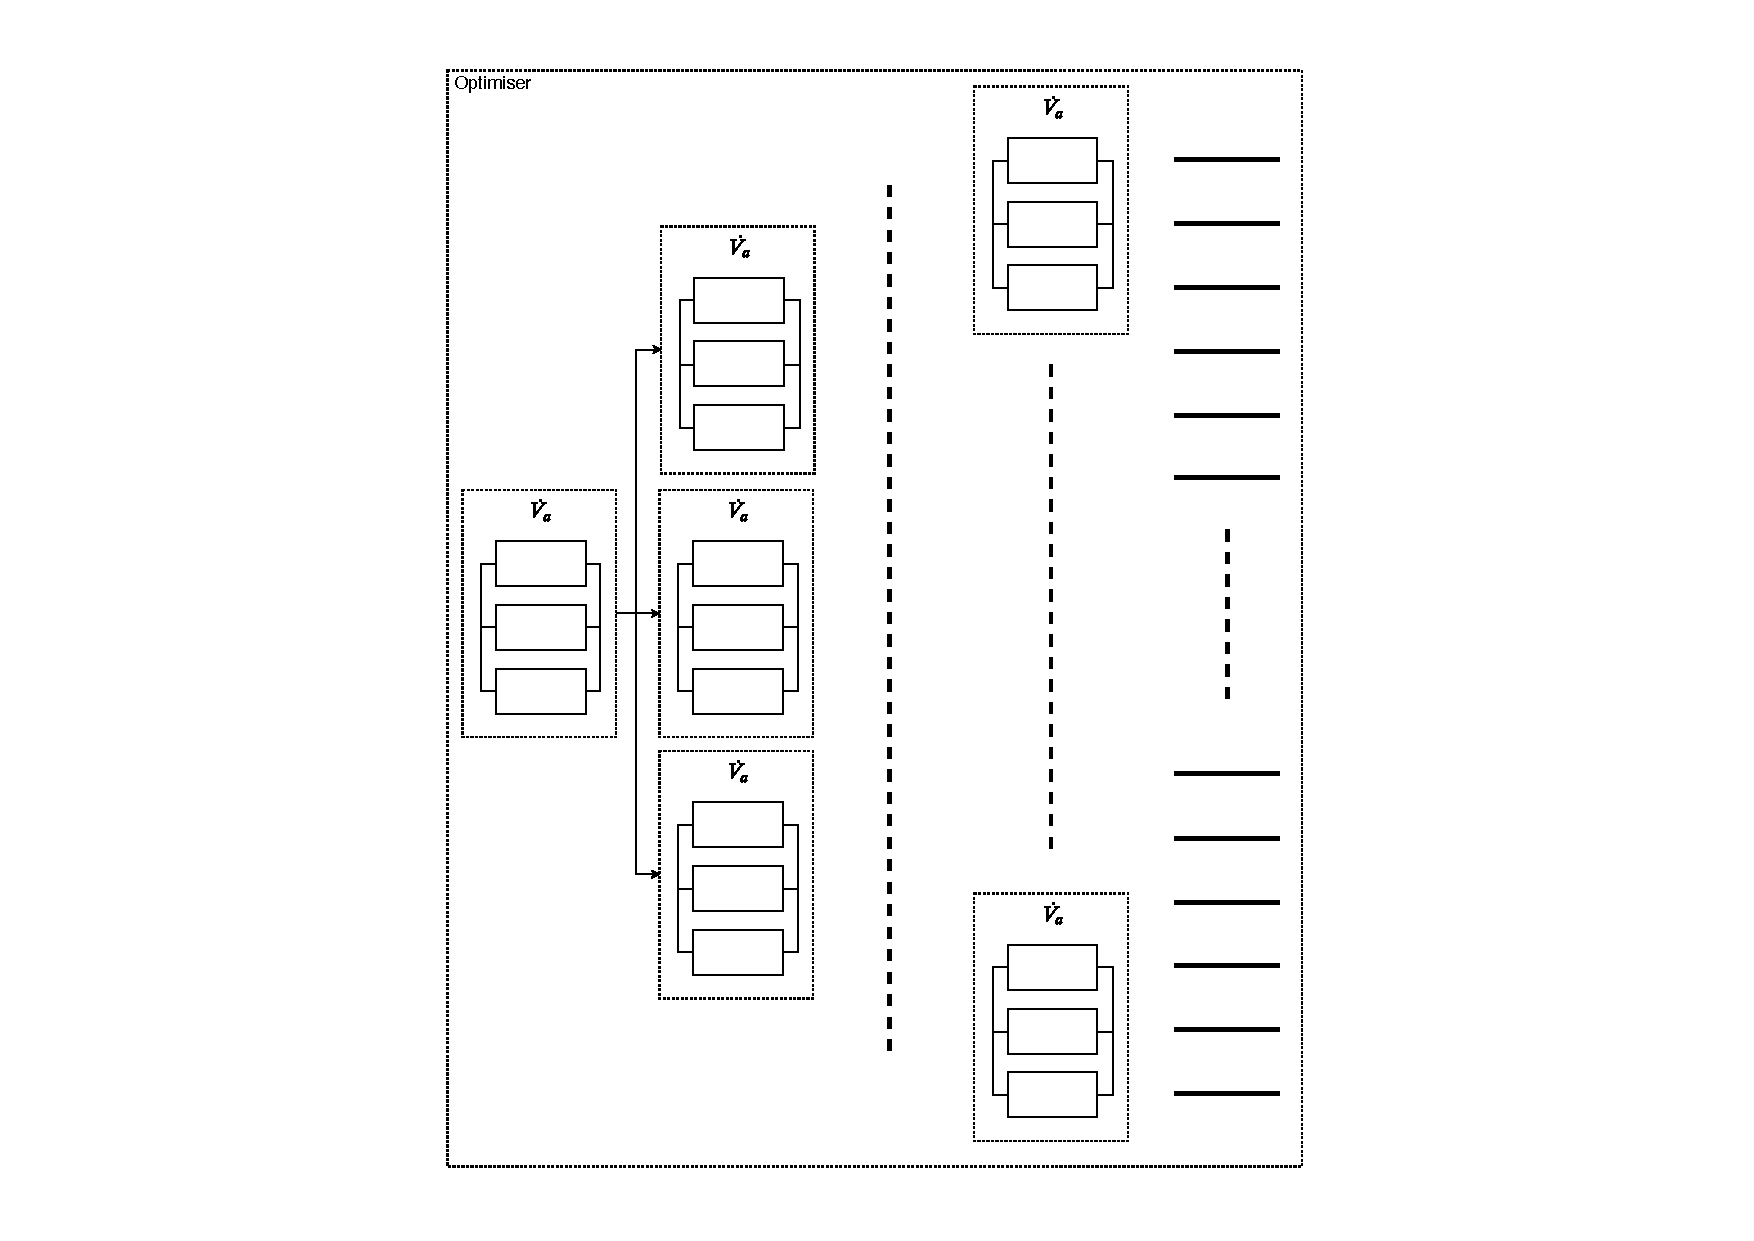
\includegraphics[clip, trim=5cm 1cm 5cm 1cm, width=1.00\textwidth]{BlockDiagram_Optimiser.pdf}
    \caption{Optimiser}
    \label{fig:control_diagram_optimiser}
\end{figure}

\clearpage
\section{Software Architecture}
\label{sub:software}


\subsection{Overview}
\label{sub:software_overview}

The design of the software architecture follows the structure shown in \Cref{fig:software_arch}. The system is comprised of three major subsystems, the low level utility interface which handles communications to the peripheral devices, the logic hardware i/o layer, and the MPC control scheme. The first subsystem, reads in sequence each of the sensors updating the data fed into the control loop as often as possible. This extracts the complicated nature of peripheral interaction into intuitive c++ classes. The second subsystem consists an instance of each joint in the system. One and two axis joints are implemented each of which contain an instance of all the muscles for that specific joint as well as a controller which takes the reference angles for the joints and drives the setpoint for each muscle. Each muscle then also contains a valve, pressure sensor and linear potentiometer associated with that muscle as well as the relevant microcontroller pins. This software structure allows all muscles to contain the same base control methods with varying parameters between them. The final sub system performs the MPC control calculations as discussed in \Cref{sub:control_system} to determine the desired valve states for each of the muscles concerned.

\begin{figure}[!hbt]
    \centering
    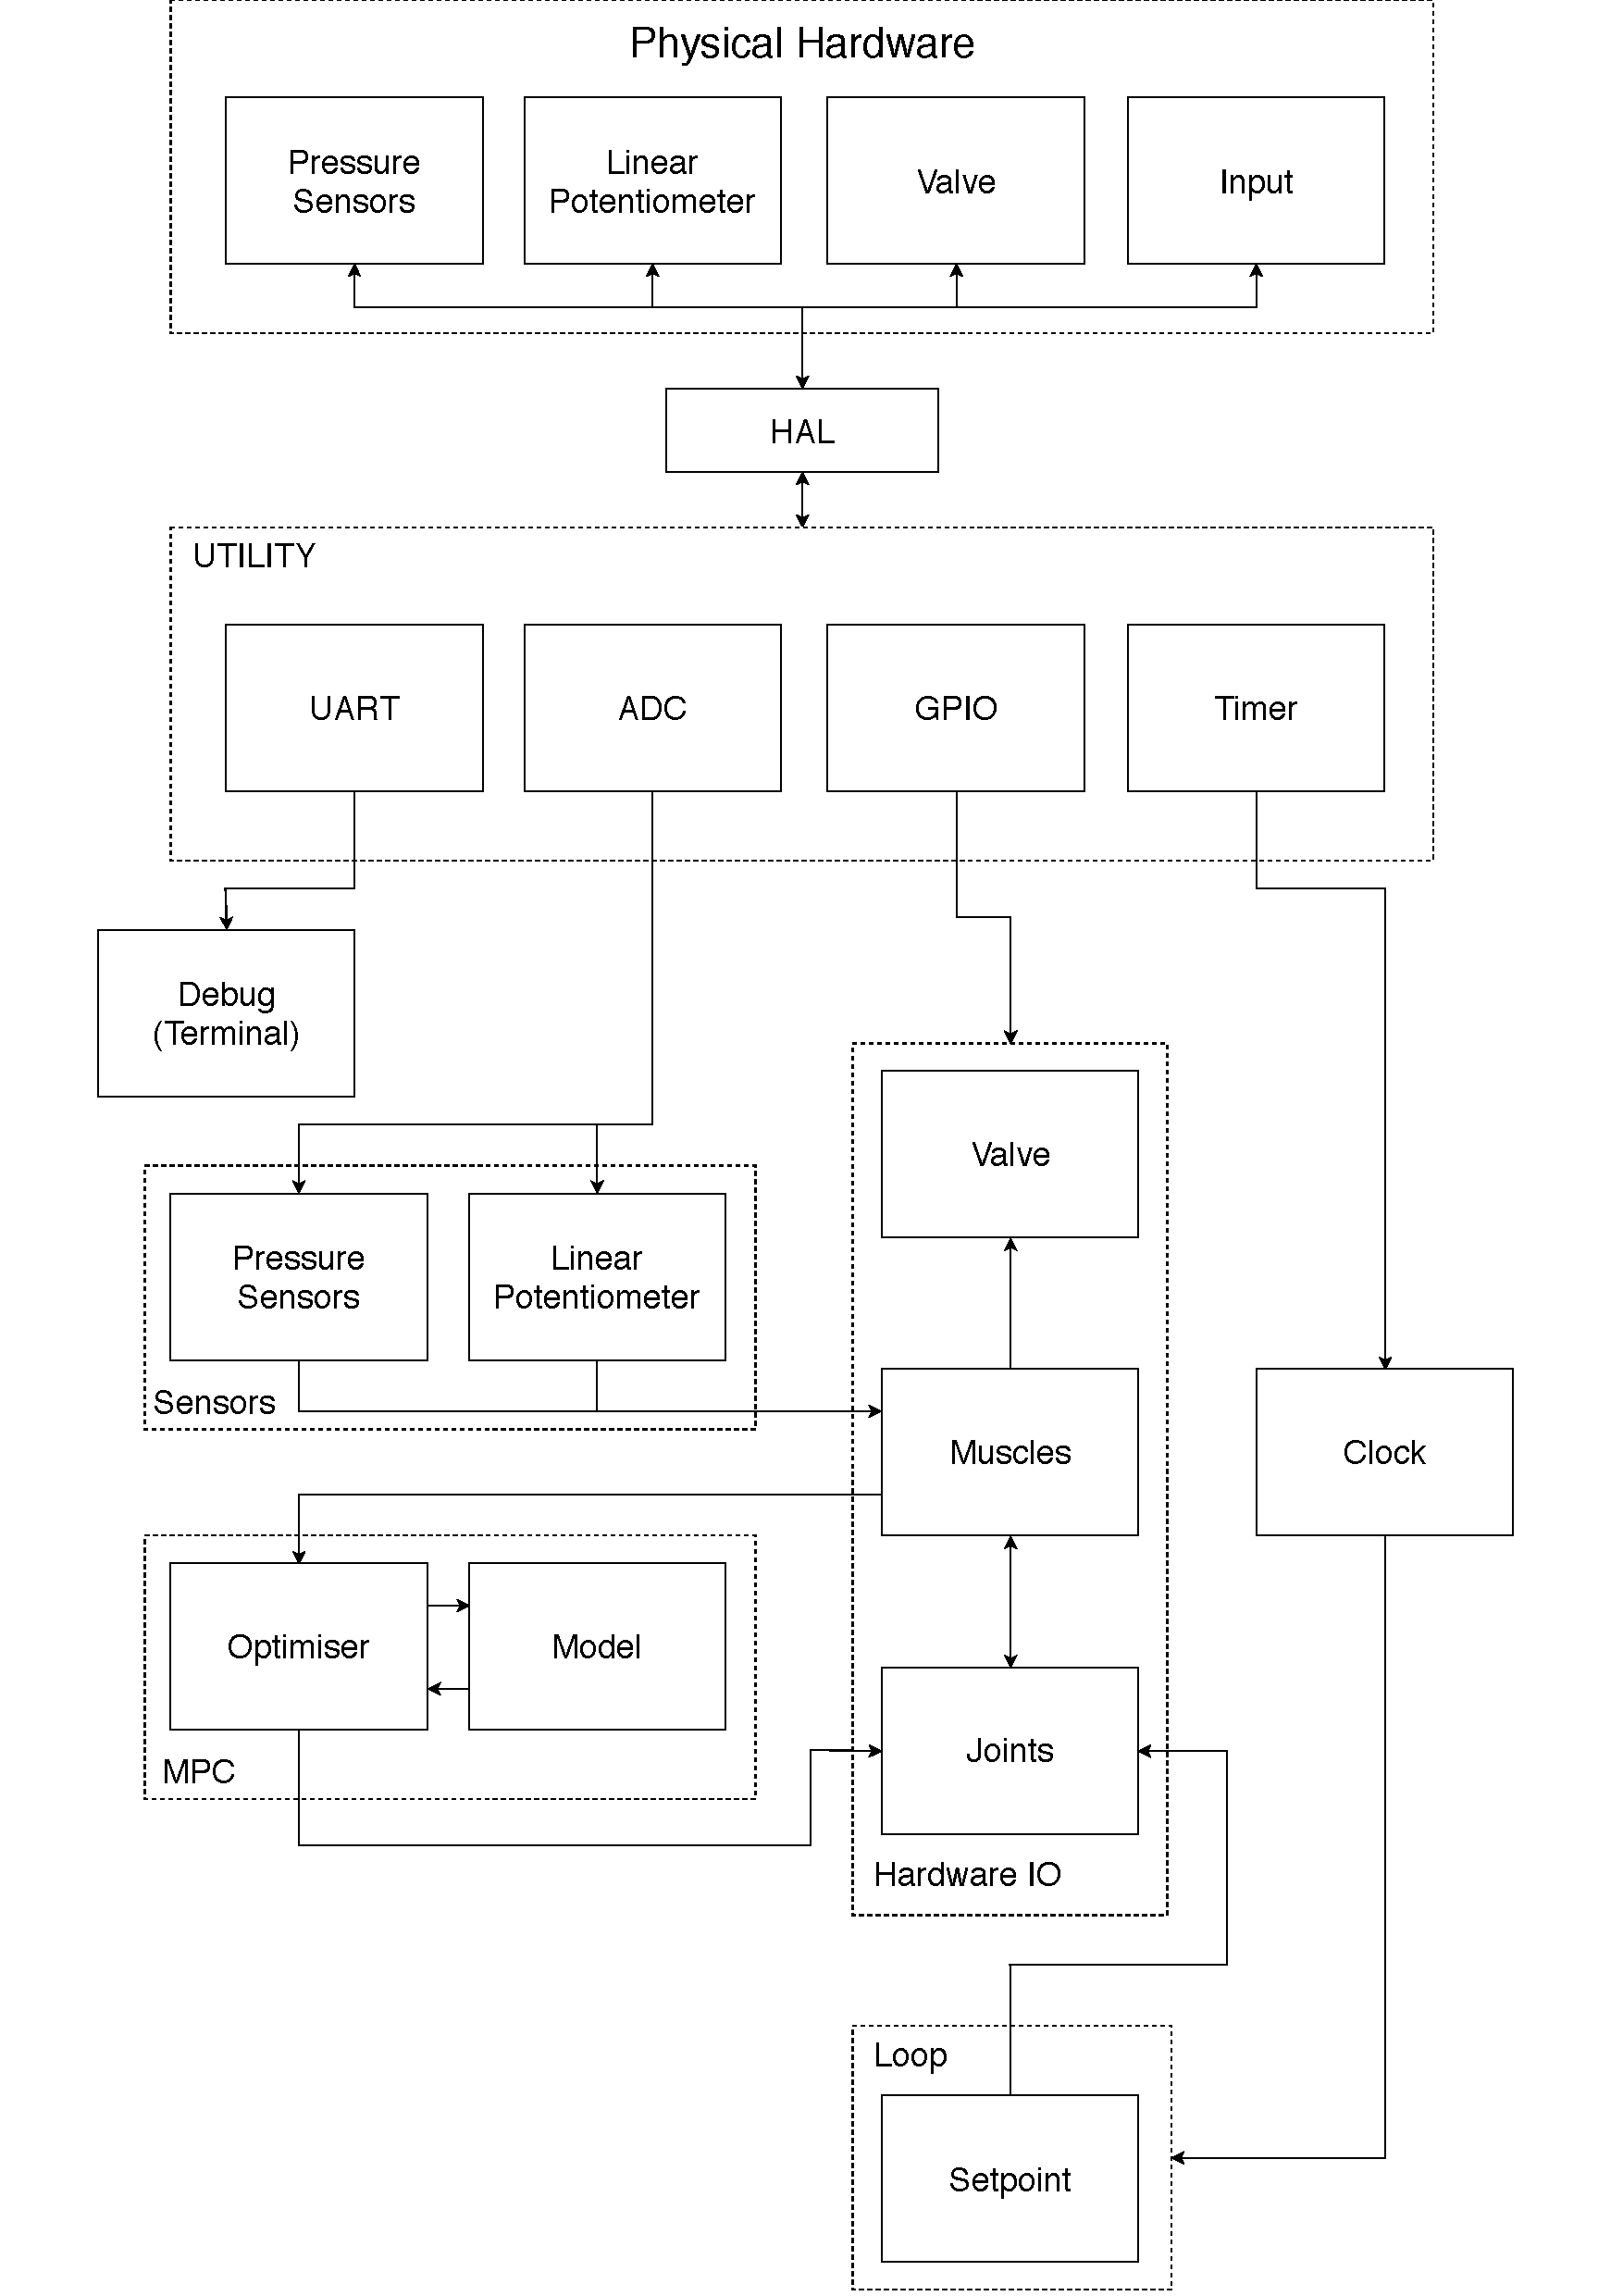
\includegraphics[clip, trim=0cm 0cm 0cm 0cm, width=1.00\textwidth]{Software.pdf}
    \caption{Software Overview}
    \label{fig:software_arch}
\end{figure}

\subsection{Control Structure}
\label{sub:control_structure}
As this project has a major focus on the framework behind an embedded systems controller, the software architecture has a strong fixation on the modularity of the subsystems. Each item in \Cref{fig:software_arch} forms an individual class open to a multitude of applications. As mention in \Cref{sub:software_overview} each joint class constructs any and all muscles required for that joint, this allows any muscle instance to be used by a joint simply by changing the specific instance the joint is constructed with. The controller used can also be changed between instances through the templated axis class and overloaded constructors. This allows for both optimiser driven controllers or more traditional controllers to be utilised. 

\begin{listing}
\begin{minted}{c++}
module::HardwareIO::joint::OneAxis<module::MPC::AdaptiveMPC::AdaptiveMPC> 
    one_axis_joint(
        muscles, 
        1, 
        0.47, 
        module::MPC::AdaptiveMPC::optimizer
    );

module::HardwareIO::joint::OneAxis<module::SMC::SMC> 
    one_axis_joint(
        muscles, 
        1, 
        0.47,
        module::SMC::smc
    );
\end{minted}
\begin{minted}{c++}
template <typename T>
class OneAxis {
public:
    OneAxis(std::vector<module::HardwareIO::muscle_t>& muscle,
        float mass,
        float radius,
        module::MPC::AdaptiveMPC::Optimizer optimizer)
    : muscle1(muscle[0]), muscle2(muscle[1]), controller(optimizer) {
    }
    
    OneAxis(std::vector<module::HardwareIO::muscle_t>& muscle, 
            float mass, 
            float radius, 
            T controller)
        : muscle1(muscle[0]), muscle2(muscle[1]), controller(controller) {
    }
    
private:
    module::HardwareIO::Muscle muscle1;
    module::HardwareIO::Muscle muscle2;
    T controller;
    axis_model_t axis_model;
};
\end{minted}
\end{listing}

\subsection{Optimiser Performance}
\label{sub:optimiser_performance}
To evaluate the feasibility of running the control structure and MPC on the embedded system a series of tests were performed. By utilising different compiler optimisations to determine whether the microcontroller would be capable of running the control structure. Tests were performed using the Debug, Release and MinSizeRel cmake build types over a range of optimiser layer depths. \Cref{fig:optimiser_process_time} shows the three build flags average process time in milliseconds. Plotted for a single prediction horizon, vs the number of layers in the optimiser. These tests were performed over 1000 iterations to ensure any processor caching was observed. Also plotted is the sampling time floor $T_s$ as the minimum process time for a new sample of data. \newline
As a result of these performance tests, to achieve a process time approximately equal to the sampling time of the system, the code should be compiled as Release with a maximum of 5 layers. This in turn implies a prediction horizon of 250 ms given a sampling time of 50 ms.

\begin{figure}[hbt!]
    \centering
    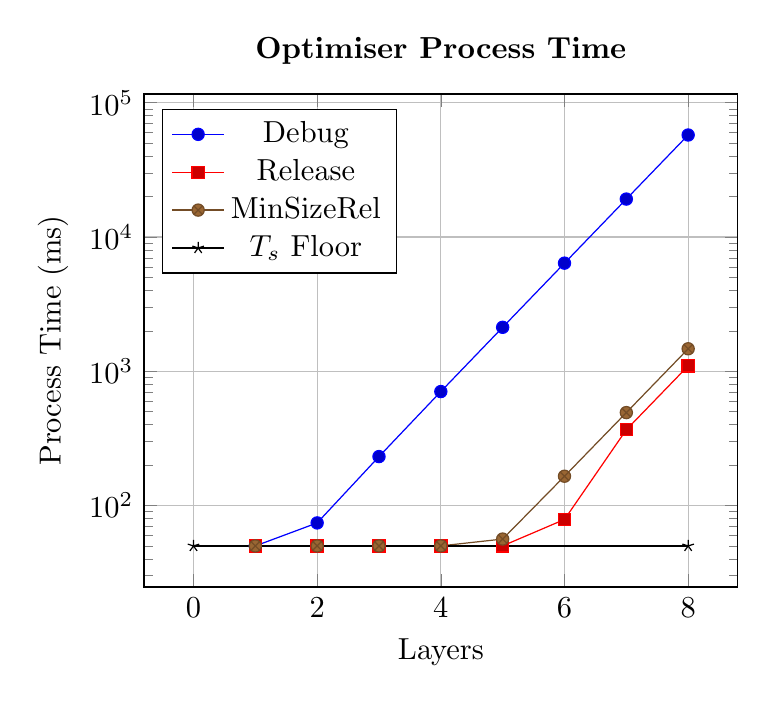
\begin{tikzpicture}[scale = 1.1]
    	\begin{semilogyaxis}[title={\textbf{Optimiser Process Time}},
    		xlabel={Layers}, ylabel={Process Time (ms)}, legend pos={north west}, grid]
    		\addplot plot coordinates {
    			(1, 50.017)
    			(2, 74.235)
    			(3, 231.597)
    			(4, 706.38)
    			(5, 2127.14)
    			(6, 6391.67)
    			(7, 19185.7)
    			(8, 57563.7)
    		};
    		\addplot plot coordinates {
    			(1, 50.017)
    			(2, 50.017)
    			(3, 50.017)
    			(4, 50.017)
    			(5, 50.068)
    			(6, 78.78)
    			(7, 366.94)
    			(8, 1097.54)
    		};
    		\addplot plot coordinates {
    			(1, 50.017)
    			(2, 50.017)
    			(3, 50.017)
    			(4, 50.058)
    			(5, 56.3)
    			(6, 165.33)
    			(7, 492.418)
    			(8, 1471.434)
    		};
    		\addplot plot coordinates {
    		    (0, 50)
    		    (8, 50)
    		};
    		\legend{Debug\\Release\\MinSizeRel\\$T_s$ Floor\\}
    	\end{semilogyaxis}
    \end{tikzpicture}
    \caption{Optimiser performance with different build types}
    \label{fig:optimiser_process_time}
\end{figure}


\clearpage
\section{Simulated System}
\label{sub:simulated_system}
To analyse the performance of the controller, a simulated hardware module was created. This module is based on the \cite{hosovsky_2012} model used in the MPC controller. Simulated sensors have been implemented with some added Gaussian measurement noise. The simulated plant is used to test the controller before experimental tests are performed. The MPC controller is compared to two other control implementations, PID and SMC, to determine the relative effectiveness of the controller.

\subsection{Simulation Results}
\label{sub:simulation_results}
Figures \Cref{fig:simulated_pid}, \Cref{fig:simulated_smc} and \Cref{fig:simulated_mpc} show the simulated responses to a reference input. These simulations were run with three controllers to compare the feasibility and tracking error of each. An implementation of PID, SMC and MPC have been compared with their tracking error on \Cref{fig:controller_tracking_error}.

\begin{figure}[!hbt]
    \centering
    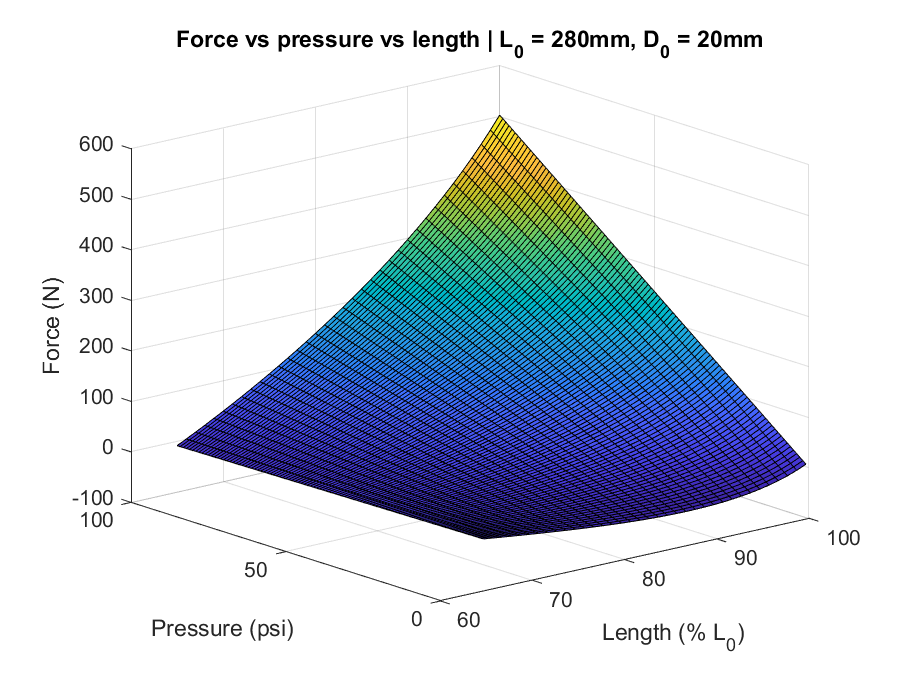
\includegraphics[scale=0.8]{staticmap.eps}
    \caption{Simulated PID controller}
    \label{fig:simulated_pid}
\end{figure}
\begin{figure}[!hbt]
    \centering
    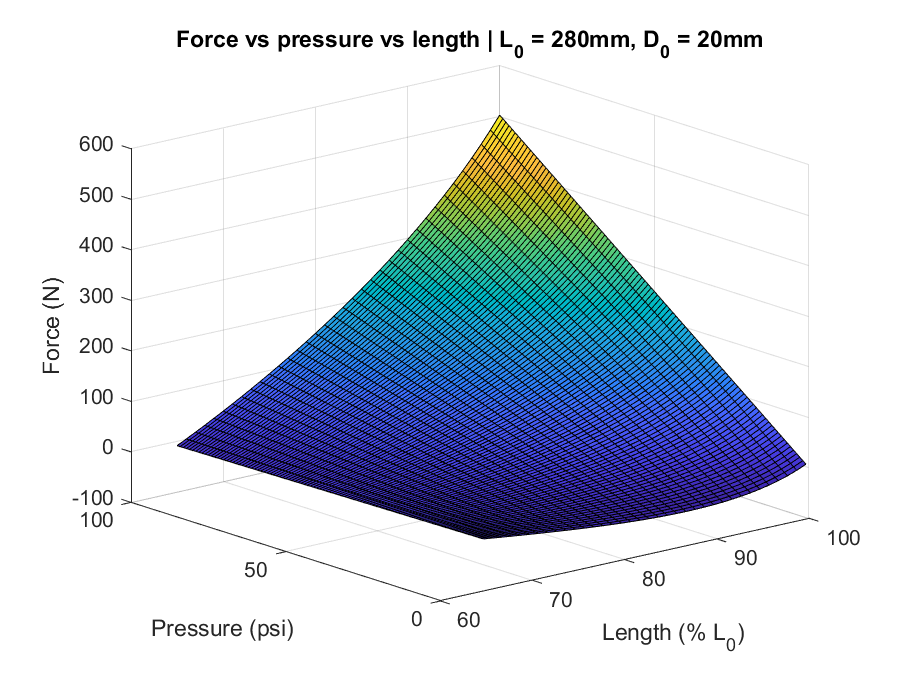
\includegraphics[scale=0.8]{staticmap.eps}
    \caption{Simulated SMC controller}
    \label{fig:simulated_smc}
\end{figure}
\begin{figure}[!hbt]
    \centering
    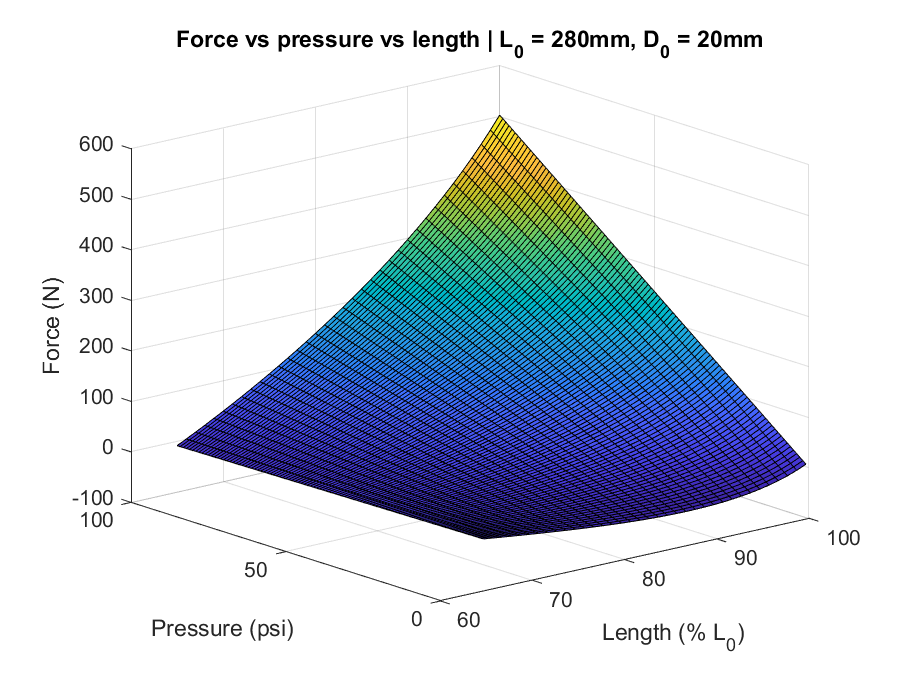
\includegraphics[scale=0.8]{staticmap.eps}
    \caption{Simulated MPC controller}
    \label{fig:simulated_mpc}
\end{figure}
\begin{figure}[!hbt]
    \centering
    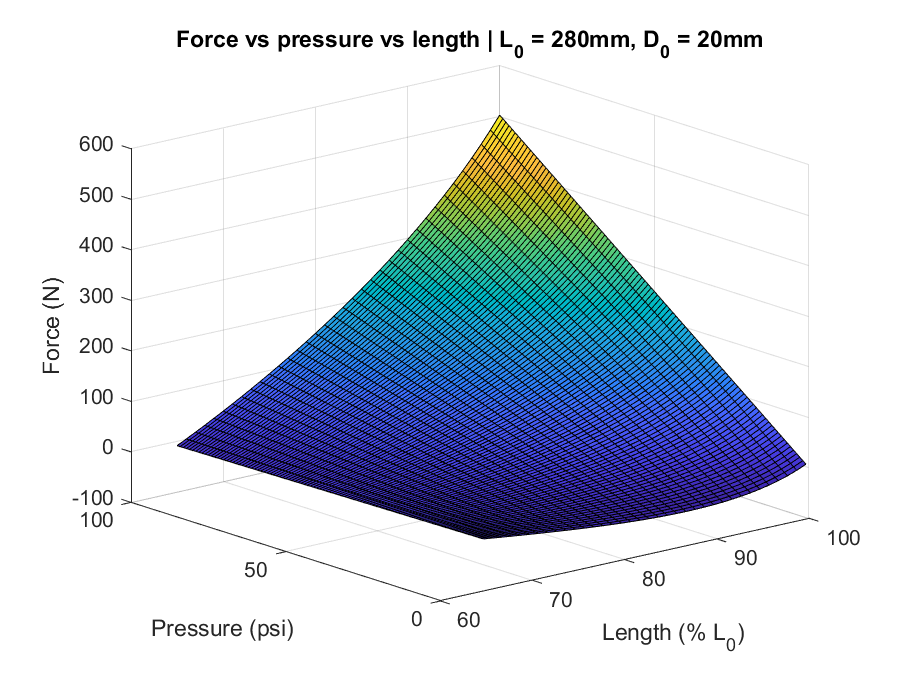
\includegraphics[scale=0.8]{staticmap.eps}
    \caption{Simulated controller tracking error comparison}
    \label{fig:controller_tracking_error}
\end{figure}

\clearpage
\section{Conclusion}
\label{sec:conclusion}
The goal of this design  will be to develop a humanoid robotic platform designed to replicate the motions of a human closer than the current electric servo driven humanoid robots. To achieve this goal an alternate actuator must be developed, and a platform feasibility study performed to determine the viability of the actuator developed. Shown in \Cref{fig:platform} this platform has been designed to mimic the range of joint movements capable by a human, this biologically inspired platform is formed around the skeleton dimensions of an adult human, implementing muscle groups to control the joints for each degree of freedom. \newline

Whilst testing actuator designs, a less than desirable lifetime for inflation/deflation cycles was observed. Three actuators failed within 10 cycles of inflation. This was due to an incompatibility between the inner bladder and the braided mesh as described in \cite{andrikopoulos_nikolakopoulos_2017}. The latex bladder used was found to have inconsistent tolerances in material thickness along the length of the sample, this resulted in nonuniform inflation of the bladder resulting in increased pressure and stress regions of the material. A more compatible set of components were discovered, with closer diameters between the bladder and braid. This consisted of an 18mm road bike tube with the previously used 20mm braid. This new pneumatic muscle was capable of lifting 16 kg under full contraction.\newline

As part of the system feasibility evaluation, the microcontroller chosen was evaluated for it's processing capability. This processor was found to be adequate for initial testing, however, for prolonged use or a more complex model, a faster processor would be required.
A smaller sampling time could be achieved if a faster processor was used, this in turn would increase the accuracy of the predictions.\newline

The static model of the two muscle constructions tested were found to not accurately represent the experimental results. This further shows the need for a more defined model for the system to behave more predictably.

\subsection{Single Degree of Freedom Joint}
\label{sub:two_dof_joint}
Further work on the project will focus on finalising the test rig implementation. This will aim to gather experimental results from the physical system. To achieve this some physical components of the system need to be tested.

\subsection{Project Extensions}
\label{sub:project_extensions}
Featured below are further extensions for future projects. These should focus on the refinement of current works. This project should provide the foundation for many extensions focusing on a variety of aspects.

\subsubsection{Multi Degree of Freedom Joint}
\label{sub:two_dof_joint}
The development of a multiple degree of freedom joint can be designed based on the foundation of the project. Reworking the model to include a second axis and set of control surfaces.

\subsubsection{Muscle Design}
\label{sub:future_muscle_design}
Further research and development could be focused on the design of the pneumatic air muscles. These could be compared to commercially available pneumatic air muscles. The performance, durability and cost could be utilised in the overall feasibility of the project.

\subsubsection{Alternative Control Methods}
\label{sub:alternative_control_methods}
Additionally, alternative control methods could be researched, improving the performance of the system. This could include model refinement if a model reliant control strategy was implemented. 


\clearpage
\begin{appendices}
\crefalias{section}{appsec}
\section{Static Force Derivation}
\label{sub:staticforcederive}
Approximating the volume as a cylinder, the dependency of the diameter on the length can be approximated by using the Pythagoras theorem 
\begin{equation}
    D(L) = \frac{\sqrt{L_{Fibre}^2-L^2}}{n \pi}
\end{equation}
This then follows that \Cref{math:diameterconst1} and \Cref{math:diameterconst2} are only dependent on the initial conditions
\begin{equation}
    n = \frac{L_0\tan(\Theta_0)}{\pi D_0}
    \label{math:diameterconst1}
\end{equation}
\begin{equation}
    L_{Fibre} = \frac{L_0}{\cos(\Theta_0)}
    \label{math:diameterconst2}
\end{equation}
Inserting the functional dependency on the diameter into the equation of a cylinder results in a volume only dependent on the length and initial conditions
\begin{equation}
    V(L) = \frac{L L_{Fibre}^2}{4 \pi n^2}-\frac{L^3}{4 \pi n^2}
\end{equation}
The virtual work of the PMA can be split into two parts, the work done by the volume of air and the elasticity of the membrane 
\begin{equation}
    W_{PMA} = W_{VAE} + W_{Elast}
\end{equation}
\begin{equation}
    \sigma_{L} = E_{RU}(L) \frac{L-L_0}{L_0}
\end{equation}
\begin{equation}
    \sigma_{PE} = E_{RU}(L) \frac{D-D_0}{D_0}
\end{equation}
\begin{equation}
    W_{L} = -\sigma_{L} H_0 \pi D(L)
\end{equation}
\begin{equation}
    W_{Elast-PE} = -\sigma_{PE} H_0 L \pi
\end{equation}
Finally the following equation gives the positive pulling force exherted by the muscle
\begin{equation}
    F_{PMA}(\rho, l) = -\rho \frac{dV}{dL}+F_{PE} \frac{dD}{dL}-F_L
    \label{math:staticforcederive}
\end{equation}

\clearpage
\section{Dynamic Force Derivation}
\label{sub:dynamicforcederive}
This derivation is taken from \cite{hosovsky_2012} and has been condensed to the relevant equations required.\newline
\begin{equation}
    \ddot{y} = \frac{1}{m}[F_E-F_S(k,P_m)-F_D(\dot{k},P_m)]
\end{equation}

\begin{gather}
 F_{CE} =
 \begin{bmatrix}
    1 \\ 
    k \\
    k^2 \\
    k^3 \\
    k^4 \\
    k^5 \\
   \end{bmatrix}
 \begin{bmatrix}
    1 & P_m & P_m^2 & P_m^3 & P_m^4 & P_m^5 \\
   \end{bmatrix}
  \begin{bmatrix}
    a_{00} & a_{01} & a_{02} & a_{03} & a_{04} & a_{05} \\
    a_{10} & a_{11} & a_{12} & a_{13} & a_{14} & 0 \\
    a_{20} & a_{21} & a_{22} & a_{23} & 0      & 0 \\
    a_{30} & a_{31} & a_{32} & 0      & 0      & 0 \\
    a_{40} & a_{41} & 0      & 0      & 0      & 0 \\
    a_{50} & 0      & 0      & 0      & 0      & 0 \\
   \end{bmatrix}
\end{gather}

\begin{equation}
    F_D(\dot{k},P_m) = -RP_m\dot{k}
\end{equation}

\begin{equation}
   \dot{V_a} = \begin{cases} 
        P_1C\sqrt{\frac{T_0}{T_1}}\sqrt{1-(\frac{\frac{P_2}{P_1}-b}{1-b})^2}, & \text{if}\ \frac{P_2}{P_1} > b\\ 
        P_1C\sqrt{\frac{T_0}{T_1}}, & \text{if}\ \frac{P_2}{P_1} \leq b \end{cases}
    \label{math:v_a}
\end{equation}

\begin{equation}
    \dot{P_m} = P_a\frac{\dot{V_a}}{V_m}-P_m\frac{\dot{V_m}}{V_m}
\end{equation}

\begin{equation}
    V_m = ak^3 + bk^2 + ck + d
\end{equation}

\begin{equation}
    \dot{V_m} = 3ak^2\dot{k} + 2bk\dot{k} + c\dot{k}
\end{equation}

Where: \newline
m - moving mass (kg)\newline
y - muscle displacement (m)\newline
$F_s(k, P_m)$ - nonlinear spring force (N)\newline
$F_d(\dot{k}, P_m)$ - nonlinear damper force (N)\newline
$F_E$ - external force (N)\newline
$k = k_0 + \frac{y}{l_0}$ - muscle contraction\newline
$k_0$ - initial muscle contraction\newline
$l_0$ - initial muscle length\newline
$P_m$ - absolute muscle pressure (Pa)\newline
$a_{xx}$ - 21 coefficient static map matrix\newline
$R$ - damping coefficient $(m^2s)$\newline
$\dot{k}$ - muscle velocity (1/s)\newline
$\dot{V_a}$ - time derivative of muscle air volume (volume flow rate through the valve) $(m^3/s)$
$P_1$ - absolute upstream pressure (Pa)\newline
$C = 2.6167x10^{-9}$ - sonic conductance $(m^3/(sPa))$\newline
$T_0$ - ambient air temperature at reference conditions (K)\newline
$T_1$ - upstream temperature (K)\newline
$P_2$ - absolute downstream pressure (Pa)\newline
b = 0.433 - critical ratio\newline
$P_a$ - atmospheric pressure (Pa)\newline
$V_a$ - volume of air in the muscle $(m^3)$\newline
$V_m$ - muscle volume $(m^3)$\newline
$\dot{V_m}$ - time derivative of muscle volume $(m^3/s)$\newline
a, b, c, d - polynomial coefficients

\clearpage
\section{Shield Schematic}
\label{sub:shieldshecmatic}
The schematic for the electronics shield used to interface the potentiometers, pressure sensors and valves. 
\begin{figure}[hbt!]
    \centering
    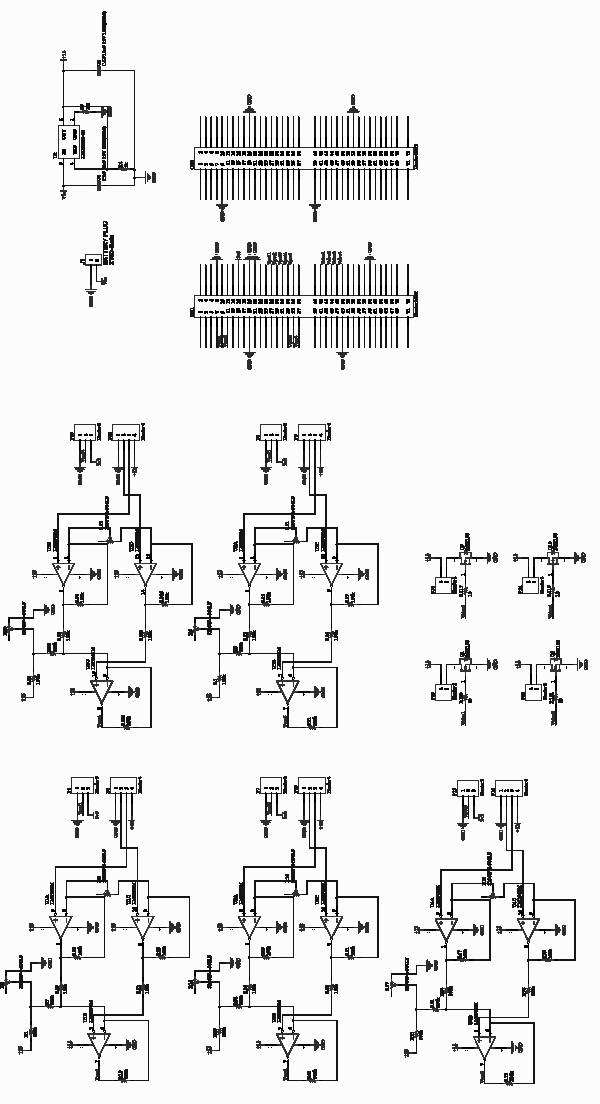
\includegraphics[origin=c, clip, trim=0cm 0cm 0cm 0cm, width=0.7\textwidth]{ShieldSCH_crop.pdf}
    \caption{Shield Schematic}
    \label{fig:shield_SCH}
\end{figure}
    
\clearpage
\section{A Matrix Derivation}
\label{sub:Amatderive}
The partial differential of each state function with respect to each state then forms the final $\boldsymbol{A}$ matrix \Cref{math:A_matrix}.
TODO Finish this
\begin{align}
    \alpha_{10} = \fdv{F_2}{z_1} &= \frac{1}{m}\left[-dk_{CE2}F_{CE2}P_{CE2}-dk_{CE1}F_{CE1}P_{CE1}\right]
    \label{math:alpha_10_matrix}\\
    \text{where}\nonumber\\
    %
    dk_{CE} &= 
    \begin{bmatrix}
        0 & 1/L_0 & 2k/L_0 & 3k^2/L_0 & 4k^3/L_0 & 5k^4/L_0
    \end{bmatrix}\nonumber\\
    F_{CE} &= 
    \begin{bmatrix}
             p_{00} & p_{01} & p_{02} & p_{03} & p_{04} & p_{05}\\
             p_{10} & p_{11} & p_{12} & p_{13} & p_{14} & 0\\
             p_{20} & p_{21} & p_{22} & p_{23} & 0      & 0\\
             p_{30} & p_{31} & p_{32} & 0      & 0      & 0\\
             p_{40} & p_{41} & 0      & 0      & 0      & 0\\
             p_{50} & 0      & 0      & 0      & 0      & 0
    \end{bmatrix}\nonumber\\
    P_{CE} &= 
    \begin{bmatrix}
        1 & P_m & P_m^2 & P_m^3 & P_m^4 & P_m^5
    \end{bmatrix}^T\nonumber\\
    k_1 &= k_{01} + y/L_{01}\nonumber\\
    k_2 &= k_{02} - y/L_{02}\nonumber
\end{align}

\begin{align}
    \alpha_{11} = \fdv{F_2}{z_2} &= \frac{1}{m}(-F_{D1} - F_{D2})
    \label{math:alpha_11_matrix}\\
    \text{where}\nonumber\\
    %
    F_D &= -RP_{m}\dot{k}\nonumber\\
    \dot{k}_1 &= 1/L_{01}\nonumber\\
    \dot{k}_2 &= -1/L_{02}\nonumber
\end{align}

\begin{align}
    \alpha_{12} = \fdv{F_2}{z_3} &= \frac{1}{m}(-F_{S1} - F_{D1})
    \label{math:alpha_12_matrix}\\
    \text{where}\nonumber\\
    %
    F_{D1} &= -R_1\dot{k}_1\nonumber\\
    \dot{k}_1 &= k_{01} + \dot{y}/L_{01}\nonumber\\
    F_{S1} &= k_{CE1} F_{CE1} dP_{CE1}\nonumber\\
    k_{CE1} &= 
    \begin{bmatrix}
        1 & k_1 & k_1^2 & k_1^3 & k_1^4 & k_1^5
    \end{bmatrix}\nonumber\\
    F_{CE1} &= 
    \begin{bmatrix}
             p_{00} & p_{01} & p_{02} & p_{03} & p_{04} & p_{05}\\
             p_{10} & p_{11} & p_{12} & p_{13} & p_{14} & 0\\
             p_{20} & p_{21} & p_{22} & p_{23} & 0      & 0\\
             p_{30} & p_{31} & p_{32} & 0      & 0      & 0\\
             p_{40} & p_{41} & 0      & 0      & 0      & 0\\
             p_{50} & 0      & 0      & 0      & 0      & 0
    \end{bmatrix}\nonumber\\
    dP_{CE1} &= 
    \begin{bmatrix}
        0 & 1 & 2P_{m1} & 3P_{m1}^2 & 4P_{m1}^3 & 5P_{m1}^4
    \end{bmatrix}^T\nonumber\\
    k_1 &= k_{01} + y/L_{01}\nonumber
\end{align}

\begin{align}
    \alpha_{13} = \fdv{F_2}{z_4} &= \frac{1}{m}(-F_{S2} - F_{D2})
    \label{math:alpha_13_matrix}\\
    \text{where}\nonumber\\
    %
    F_{D1} &= -R_2\dot{k_2}\nonumber\\
    \dot{k_2} &= k_{02} + \dot{y}/L_{02}\nonumber\\
    F_{S2} &= k_{CE2} F_{CE2} dP_{CE2}\nonumber\\
    k_{CE2} &= 
    \begin{bmatrix}
        1 & k_2 & k_2^2 & k_2^3 & k_2^4 & k_2^5
    \end{bmatrix}\nonumber\\
    F_{CE2} &= 
    \begin{bmatrix}
             p_{00} & p_{01} & p_{02} & p_{03} & p_{04} & p_{05}\\
             p_{10} & p_{11} & p_{12} & p_{13} & p_{14} & 0\\
             p_{20} & p_{21} & p_{22} & p_{23} & 0 &   0\\
             p_{30} & p_{31} & p_{32} & 0 &   0 &   0\\
             p_{40} & p_{41} & 0 &   0 &   0 &   0\\
             p_{50} & 0 &   0 &   0 &   0 &   0
    \end{bmatrix}\nonumber\\
    dP_{CE2} &= 
    \begin{bmatrix}
        0 & 1 & 2P_{m2} & 3P_{m2}^2 & 4P_{m2}^3 & 5P_{m2}^4
    \end{bmatrix}^T\nonumber\\
    k_{2} &= k_{02} + y/L_{02}\nonumber
\end{align}

\begin{align}
    \alpha_{20} = \fdv{F_3}{z_1} &= \frac{P_aV_{a1}}{dV_{m1}}-\frac{z_3d\dot{V}_{m1}}{dV_{m1}}\\
    \label{math:alpha_20_matrix}\\
    \text{where}\nonumber\\
    %
    dV_{m1} &= \frac{3ak^2}{L_0}+\frac{2bk}{L_0}+\frac{c}{L_0}\nonumber\\
    z_3\frac{d\dot{V}_{m1}}{dV_{m1}} &= \frac{(ak^3+bk^2+ck+d)(6ak\dot{k}+2b\dot{k})-(3ak^2\dot{k}+2bk\dot{k}+c\dot{k})(3ak^2+2bk+c)}{L_0(ak^3+bk^2+ck+d)^2}\nonumber\\
    k_1 &= k_{01} + y/L_{01}\nonumber\\
    \dot{k}_1 &= k_{01} + \dot{y}/L_{01}\nonumber\\
    \dot{V_a} &= 
    \begin{cases} 
        P_1C\sqrt{\frac{T_0}{T_1}}\sqrt{1-(\frac{\frac{P_2}{P_1}-b}{1-b})^2}, & \text{if}\ \frac{P_2}{P_1} > b\\ 
        P_1C\sqrt{\frac{T_0}{T_1}}, & \text{if}\ \frac{P_2}{P_1} \leq b
    \end{cases}\nonumber
\end{align}

\begin{align}
    \alpha_{21} = \fdv{F_3}{z_2} &= -z_3\dot{V_{m1}}/V_{m1}
    \label{math:alpha_21_matrix}\\
    \text{where}\nonumber\\
    %
    \dot{V_m1} &= 3a_1k_1^2/L_{01} + 2b_1k_1/L_{01} + c_1/L_{01}\nonumber\\
    V_{m1} &= a_1k_1^3 + b_1k_1^2 + c_1k_1 + d_1\nonumber\\
    k_1 &= k_{01} + y/L_{01}\nonumber
\end{align}

\begin{align}
    \alpha_{22} = \fdv{F_3}{z_3} &= P_a*dV_a1/V_m1 - dV_m1/V_m1
    \label{math:alpha_22_matrix}\\
    \text{where}\nonumber\\
    % 
    V_{m1} &= a_1k_1^3 + b_1k_1^2 + c_1k_1 + d_1\nonumber\\
    \dot{V}_{m1} &= 3a_1k_1^2\dot{k}_1 + 2b_1k_1\dot{k}_1 + c_1\dot{k}_1\nonumber\\
    k_1 &= k_{01} + y/L_{01}\nonumber\\
    \dot{k}_1 &= k_{01} + \dot{y}/L_{01}\nonumber\\
    % \dot{V_a} &=
    % \begin{cases}
    %     \begin{cases}
    %     C\sqrt{\frac{T_0}{T_1}}\sqrt{1-\left(\frac{\frac{P_2}{P_1}-b}{1-b}\right)^2} + ((C\sqrt{\frac{T_0}{T_1}}\sqrt(\frac{P1_2}{P1_1} - b))/{1 - b}^2P1_1\sqrt{1-(\frac{\frac{P_2}{P_1}-b}{1-b})^2})
    %     , & \text{if}\ \frac{P_2}{P_1} > b\\ 
    %     C*\sqrt{\frac{T_0}{T_1}}
    %     , & \text{if}\ \frac{P_2}{P_1} \leq b
    %     \end{cases}\text{if mode 1}\ \\
    %     \begin{cases}
    %     -(C\sqrt{\frac{T_0}{T_1}}\sqrt(P1_2/P1_1 - b))/{1 - b}^2P1_1\sqrt{1-\frac{\frac{P_2}{P_1}-b}{1-b}^2}
    %     , & \text{if}\ \frac{P_2}{P_1} > b\\ 
    %     0
    %     , & \text{if}\ \frac{P_2}{P_1} \leq b
    %     \end{cases}\text{if mode 2 or 3}\ 
    % \end{cases}\nonumber\\
\end{align}

\begin{align}
    \alpha_{30} = \fdv{F_4}{z_1} &=
    \label{math:alpha_30_matrix}\\
    \text{where}\nonumber\\
%     dk2 = k_02 - dy/L_02;
% dV_m2 = c2/L_02 + 2*b2*dk2/L_02 + 6*a2*k2*dk2/L_02;
% k2 = k_02 + y/L_02;
% V_m2 = c2/L_02 + 2*b2*k2/L_02 + 3*a2*k2^2/L_02;
% if P2_2/P2_1 > b
%     V_a2 = P2_1*C*sqrt(T_0/T_1)*sqrt(1-((P2_2/P2_1 - b)/(1 - b))^2);
% else
%     V_a2 = P2_1*C*sqrt(T_0/T_1);
% end
% dF4dz1 = P_a*V_a2/V_m2 - P_m2*dV_m2/V_m2;
\end{align}

\begin{align}
    \alpha_{31} = \fdv{F_4}{z_2} &=
    \label{math:alpha_31_matrix}\\
    \text{where}\nonumber\\
%     k2 = k_02 - y/L_02;
% V_m2 = a2*k2^3 + b2*k2^2 + c2*k2 + d2;
% dV_m2 = 3*a2*k2^2/L_02 + 2*b2*k2/L_02 + c2/L_02;
% dF4dz2 = -P_m2*dV_m2/V_m2;
\end{align}

\begin{align}
    \alpha_{33} = \fdv{F_4}{z_4} &=
    \label{math:alpha_33_matrix}\\
    \text{where}\nonumber\\
%     dk2 = k_02 - dy/L_02;
% dV_m2 = 3*a2*k2^2*dk2 + 2*b2*k2*dk2 + c2*dk2;
% k2 = k_02 - y/L_02;
% V_m2 = a2*k2^3 + b2*k2^2 + c2*k2 + d2;
% dV_a2 = 0;
% if mode == 1 
%     if P2_2/P2_1 > b
%         dV_a2 = C*sqrt(T_0/T_1)*sqrt(1-((P2_2/P2_1 - b)/(1 - b))^2) + ((C*sqrt(T_0/T_1)*sqrt(P2_2/P2_1 - b))/(1 - b)^2*P2_1*sqrt(1-((P2_2/P2_1 - b)/(1 - b))^2));
%     else
%         dV_a2 = C*sqrt(T_0/T_1);
%     end
% elseif mode == 2 || 3
%     if P2_2/P2_1 > b
%         dV_a2 = -((C*sqrt(T_0/T_1)*sqrt(P2_2/P2_1 - b))/(1 - b)^2*P2_1*sqrt(1-((P2_2/P2_1 - b)/(1 - b))^2));
%     else
%         dV_a2 = 0;
%     end
% end
% dF4dz4 = P_a*dV_a2/V_m2 - dV_m2/V_m2;
\end{align}

Where: \newline
m - moving mass (kg)\newline
y - muscle displacement (m)\newline
$F_s(k, P_m)$ - nonlinear spring force (N)\newline
$F_d(\dot{k}, P_m)$ - nonlinear damper force (N)\newline
$F_E$ - external force (N)\newline
$k = k_0 + \frac{y}{l_0}$ - muscle contraction\newline
$k_0$ - initial muscle contraction\newline
$l_0$ - initial muscle length\newline
$P_m$ - absolute muscle pressure (Pa)\newline
$a_{xx}$ - 21 coefficient static map matrix\newline
$R$ - damping coefficient $(m^2s)$\newline
$\dot{k}$ - muscle velocity (1/s)\newline
$\dot{V_a}$ - time derivative of muscle air volume (volume flow rate through the valve) $(m^3/s)$
$P_1$ - absolute upstream pressure (Pa)\newline
$C = 2.6167x10^{-9}$ - sonic conductance $(m^3/(sPa))$\newline
$T_0$ - ambient air temperature at reference conditions (K)\newline
$T_1$ - upstream temperature (K)\newline
$P_2$ - absolute downstream pressure (Pa)\newline
b = 0.433 - critical ratio\newline
$P_a$ - atmospheric pressure (Pa)\newline
$V_a$ - volume of air in the muscle $(m^3)$\newline
$V_m$ - muscle volume $(m^3)$\newline
$\dot{V_m}$ - time derivative of muscle volume $(m^3/s)$\newline
a, b, c, d - polynomial coefficients

\clearpage
\end{appendices}

% \clearpage
%%% Display the bibliography.
\printbibliography
\end{document}